\documentclass{report}
\usepackage{amsmath}
\usepackage{amssymb}
\usepackage{amsfonts}
\usepackage{graphicx} 
\usepackage{verbatim}
\usepackage{enumerate}
\usepackage{multicol}
\usepackage[a4paper,margin=2.5cm]{geometry}
\linespread{1.2}

\title{Reti di telecomunicazioni}
\author{sav}
\date{2025}

\begin{document}

\maketitle
\tableofcontents


%\chapter{Conoscenze di base}
%\section{Informatica}
\subsection{Conversione binario esadecimale}
La conversione numerica si ottiene raggruppando i bit del numero binario in gruppi da quattro a partire dal punto e in entrambe le direzioni, sostituendo poi ogni gruppo di 4 bit con l'equivalente cifra del sistema esadecimale.
\begin{multicols}{4}
\begin{itemize}
    \item 0000 = 0
    \item 0001 = 1
    \item 0010 = 2
    \item 0011 = 3
    \item 0100 = 4
    \item 0101 = 5
    \item 0110 = 6
    \item 0111 = 7
    \item 1000 = 8
    \item 1001 = 9
    \item 1010 = A
    \item 1011 = B
    \item 1100 = C
    \item 1101 = D
    \item 1110 = E
    \item 1111 = F
\end{itemize}
\end{multicols}
\subsection{Tipologia reti}
Le reti di telecomunicazione sono costituite da un insieme di nodi e rami che consentono la trasmissione di informazioni tra i vari nodi. Le reti possono essere classificate in base a diversi criteri:
\begin{itemize}
    \item \textbf{Estensione geografica:}
    \begin{itemize}
        \item \textbf{PAN} (Personal Area Network): copre pochi metri, ad esempio collegamento tra dispositivi personali (Bluetooth).
        \item \textbf{LAN} (Local Area Network): copre un edificio o un campus, tipicamente reti aziendali o domestiche.
        \item \textbf{MAN} (Metropolitan Area Network): copre una città o un'area metropolitana.
        \item \textbf{WAN} (Wide Area Network): copre aree geografiche molto estese, anche nazioni o continenti (es. Internet).
    \end{itemize}
    
    \newpage
    \item \textbf{Topologia:}
    \begin{itemize}
        \item \textbf{Bus}: tutti i nodi sono collegati a un unico canale di comunicazione.
        \item \textbf{Stella}: tutti i nodi sono collegati a un nodo centrale.
        \item \textbf{Anello}: i nodi sono collegati in modo circolare.
        \item \textbf{Maglia (mesh)}: ogni nodo è collegato a più nodi, anche direttamente.
        \item \textbf{Albero}: struttura gerarchica a livelli.
        \item \textbf{Catena (chain)}: i nodi sono collegati in sequenza lineare.
        \item \textbf{Full mesh}: ogni nodo è collegato a tutti gli altri nodi.
    \end{itemize}

\end{itemize}
\subsubsection{Nodi e rami}
I nodi e i rami(link) sono gli elementi che costituiscono una rete. I nodi sono i punti di intersezione tra i rami e possono essere di diversi tipi:
\begin{itemize}
    \item Host: un nodo che genera o consuma informazioni
    \item Router: un nodo che instrada le informazioni tra i vari host
    \item Switch: un nodo che instrada le informazioni tra i vari host, ma a livello di collegamento
    \item Bridge: un nodo che collega due reti locali
    \item Gateway: un nodo che collega due reti diverse
\end{itemize}
Il ramo è il sistema trasmissivo che consente il trasporto delle
unità informative da nodo a nodo secondo tre possibili modalità di trasmissione:
\begin{itemize}
    \item simplex(unidirezionale): un solo verso di trasmissione, esempio: radio
    \item half-duplex(bidirezionale alternato): due direzioni di trasmissione, ma non contemporaneamente, esempio: walkie-talkie
    \item full-duplex(bidirezionale contemporanea): due direzioni di trasmissione contemporaneamente, esempio: telefono
    \item broadcast: un nodo invia informazioni a tutti gli altri nodi della rete, esempio: radio
\end{itemize}

\paragraph{Modalità di invio dati}
\begin{itemize}
    \item broadcast: un nodo invia informazioni a tutti i nodi della rete, esempio: radio
    \item multicast: un nodo invia informazioni a un gruppo di nodi della rete, esempio: videoconferenza
    \item unicast: un nodo invia informazioni a un solo nodo della rete, esempio: email
    \item point-to-point: un nodo invia informazioni a un altro nodo della rete, esempio: telefono
\end{itemize}

\subsubsection{Reti di accesso e reti di trasporto}
Se mando una richiesta sul web tramite il mio router di casa, collegandomi alla rete tim(rete di accesso), da quel punto in poi tim si appoggerà ad un’altra rete per rispondere alla mia richiesta(rete di trasporto), quindi è possibile distinguere velocità differenti: 
\begin{itemize}
    \item velocità di accesso(relativa ai dati che viaggiano nella rete di accesso, tipicamente agli utenti semplici non viene garantita una velocità minima(da casa non abbiamo questa garanzia), nella rete di trasporto invece viene garantita(contratto SLA))
    \item velocità di trasporto(relativa ai dati che viaggiano nella rete di trasporto)
\end{itemize}

%\subsection{Da analogico a digitale}
%in base al tipo di comunicazione decido il modo con il quale mettere in comunicazione gli utenti, se sono tanti o pochi, se sono distanti o vicini, se comunicano contemporaneamente oppure no.
%quando l'informazione che voglio trasmettere la digitallizzo, passando da analogico a digitale, ho molti vantaggi:
%campionando il segnale analogico posso ricorstruirlo in segnale digitale, in bit.
%quando chiamo qualcuno avviene il campionamento dell'onda audio della voce, questo avviene tramite il filtro passa banda tra le frequenze 300hz e 3400 hz. le alte e le bassissime frequenze vengono tagliate. 8 bit per campione, 64bit per secondo, quindi 8 campioni al secondo. la trasmissione nel canale telefonico avviene con la trasmissione di pacchetti.

\subsection*{Differenza tra quantità di valori rappresentabili e byte occupati in memoria}

Quando si lavora con i dati binari, è importante distinguere tra:

\begin{itemize}
  \item \textbf{Quantità di valori rappresentabili}: indica il numero di combinazioni possibili che si possono ottenere con un certo numero di bit. Ad esempio, con $n$ bit si possono rappresentare $2^n$ valori distinti. Questo determina l'intervallo dei numeri che si possono codificare. Ad esempio, con 16 bit (senza segno) si possono rappresentare i numeri interi da $0$ a $2^{16}-1 = 65535$.

  \item \textbf{Byte occupati in memoria}: rappresenta lo spazio fisico necessario per memorizzare quel valore. Poiché 1 byte corrisponde a 8 bit, un valore a 16 bit occupa esattamente 2 byte in memoria. Questo è indipendente dai valori specifici che si possono rappresentare con quei bit.
\end{itemize}

\noindent In sintesi, \emph{la quantità di valori rappresentabili dipende dal numero di bit}, mentre \emph{i byte occupati in memoria dipendono da come è strutturato il campo nella memoria del computer}. Un campo a 16 bit occupa sempre 2 byte, ma può rappresentare fino a 65536 valori distinti (da 0 a 65535 nel caso senza segno).



\section{Matematica}
\subsection{Potenza di due}
\begin{figure}[h!]
    \centering
    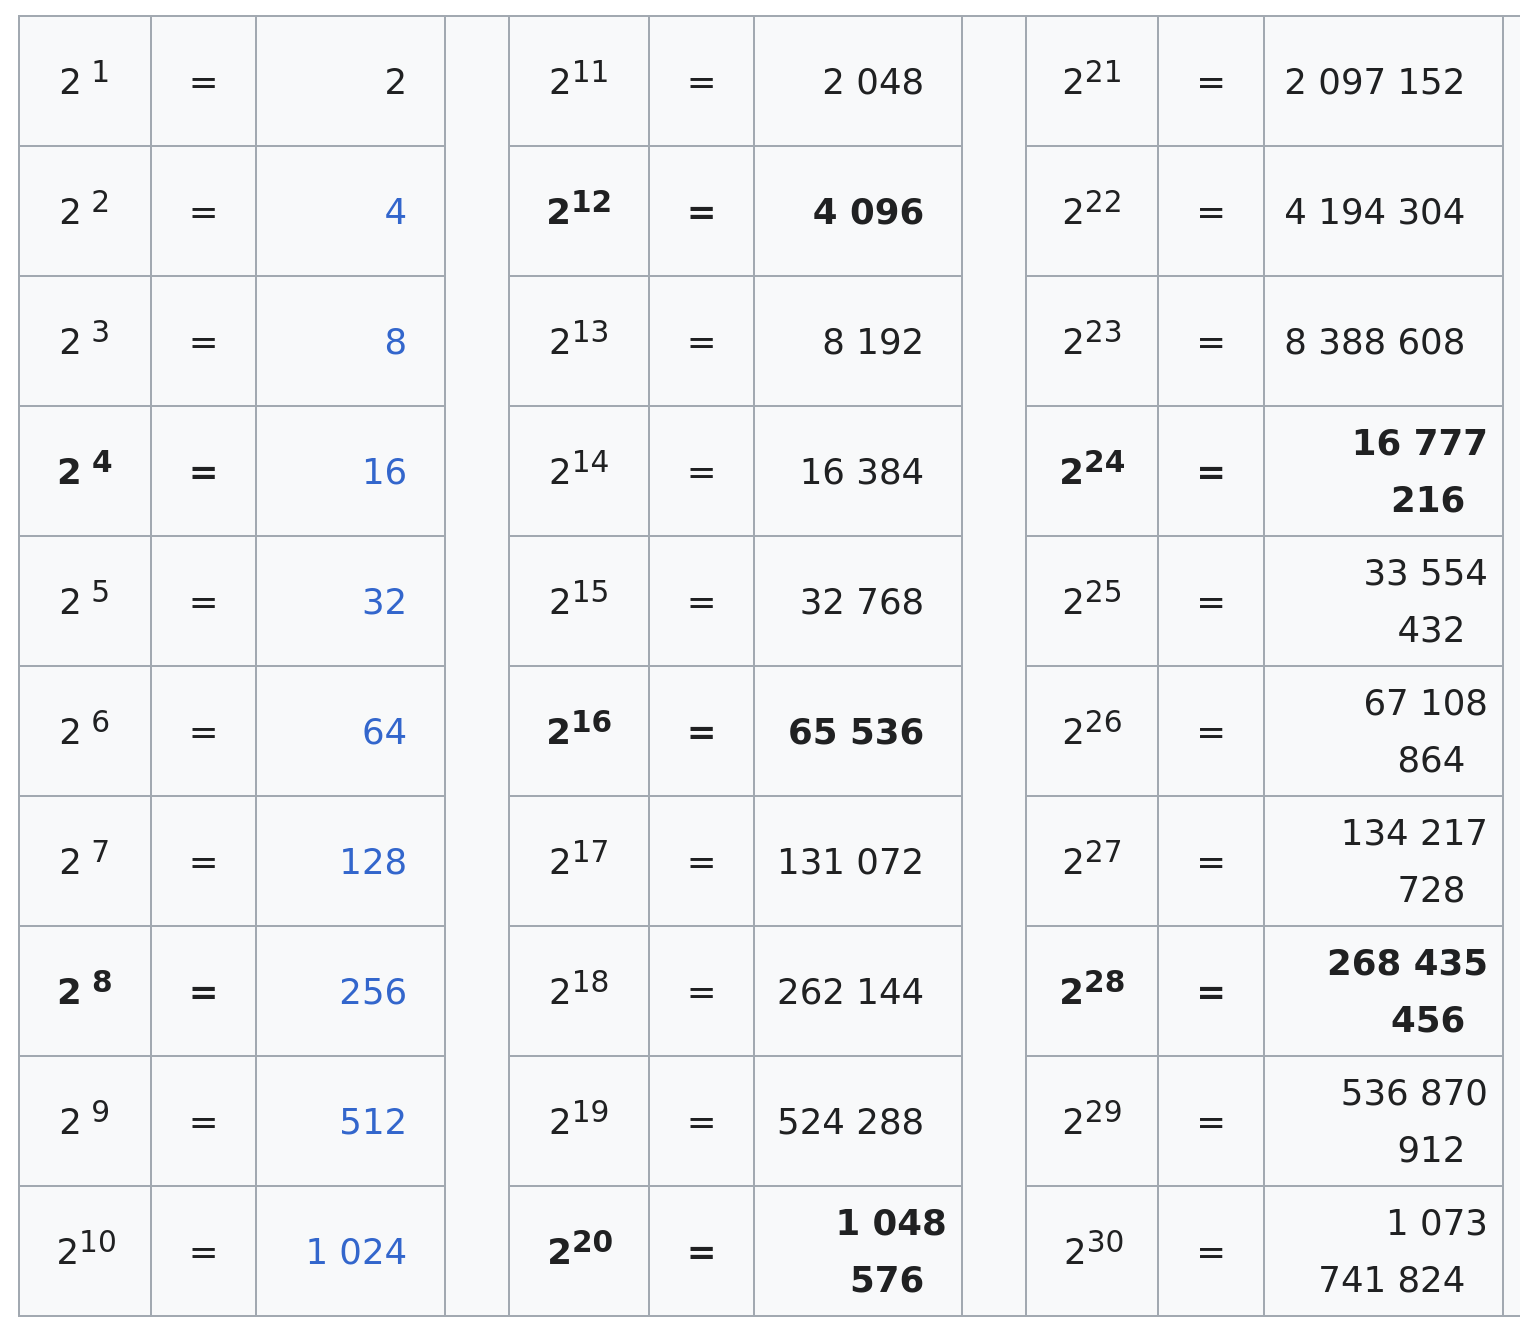
\includegraphics[width=0.8\textwidth]{images/potenza_due}
    \caption{Tabella delle potenze di due}
    \label{fig:potenza_due}
\end{figure}
\newpage
\subsection{Complemento a 1 - NOT}
Il complemento a 1  è una rappresentazione binaria in cui ogni bit di un numero binario viene invertito. Ad esempio, il complemento a 1 di 1010 è 0101. Questo metodo è spesso utilizzato per rappresentare numeri negativi nei sistemi binari.
\begin{figure}[h!]
    \centering
    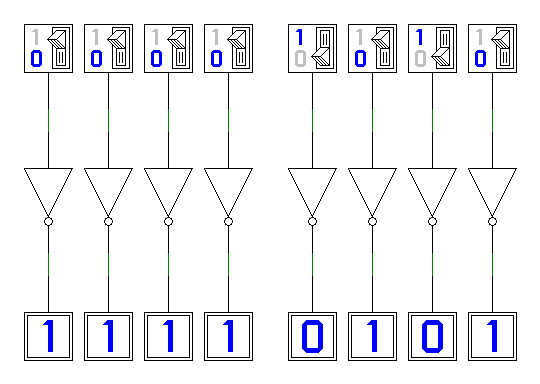
\includegraphics[width=0.6\textwidth]{images/complemento_uno}
    \caption{Esempio di complemento a 1}
    \label{fig:complemento_uno}
\end{figure}
\subsection{Aritmetica a 2 - XOR}
XOR è un operatore logico, chiamato anche OR esclusivo, che restituisce TRUE solo se uno e solo uno dei suoi operandi è TRUE.
\begin{figure}[h!]
    \centering
    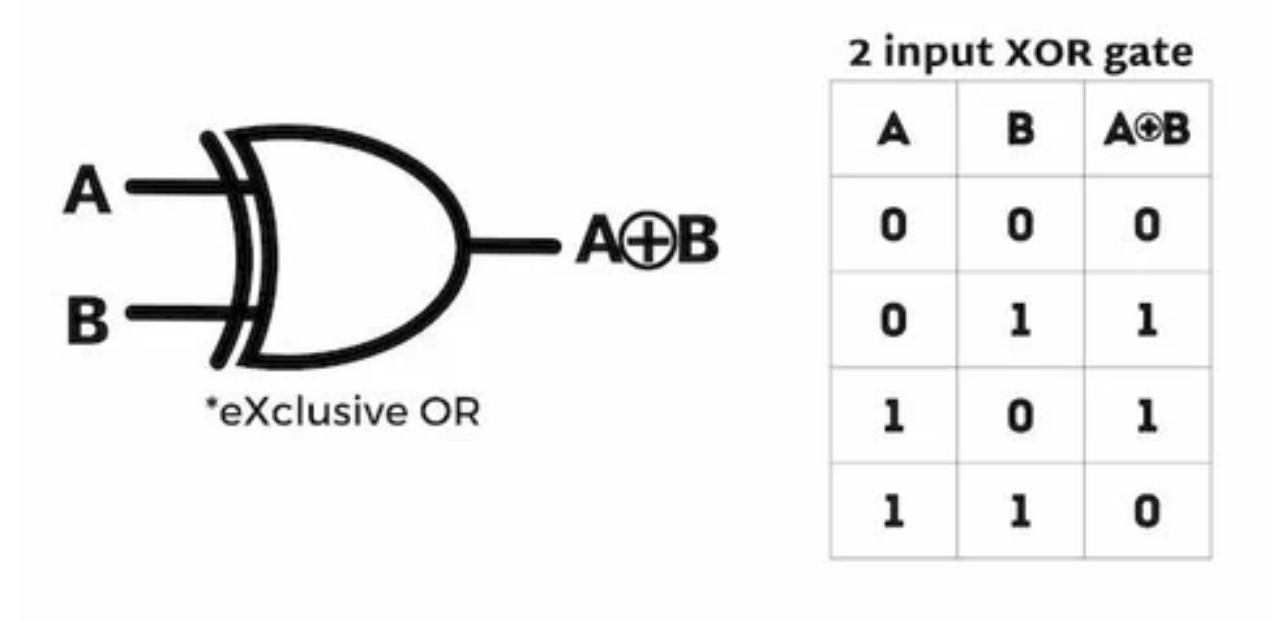
\includegraphics[width=0.6\textwidth]{images/xor.png}
    \caption{Esempio di operazione XOR}
    \label{fig:xor_example}
\end{figure}



\newpage
\section{Fisica}
\subsection{Comunicazione radio, cablata e ottica}
la trasmissione di un segnale a distanza avviene attraverso le onde elettromagnetiche, che siano trasmesse tramite antenne e quindi che si propaghino nel vuoto oppure in un cavo di fibra ottica, che anchesso trasmette la luce, quindi l’onda em.
dopo aver trasformato l'informazione in bit(codifica) questa viene trasmessa in dei canali(radio, mezzi guidati). quella radio avviene nello spazio libero(attraverso l’aria o nel vuoto), mezzi guidati(cavi)
\begin{itemize}
    \item Mezzi guidati: cavi coassiali, cavi in fibra ottica, cavi in rame
    \item Mezzi non guidati: onde radio, microonde, infrarossi
    \item Mezzi ottici: fibra ottica
\end{itemize}
\paragraph{Pro e contro del canale radio}
\begin{itemize}    
    \item Pro: risparmio sul mezzo fisico(l’aria e il vuoto sono gratis), un segnale radio non ha confini, può arrivare all’infinito, teoricamente. a noi interessa che il segnale elettromagnetico arrivi dove voglio e che venga decodificato correttamente, e non a infinito. 
un antenna è un dispositivo che genera un campo magnetico(è un pezzo di ferro su cui scorre della corrente e che quindi genera un campo magnetico, fisica 2), aiuta la comunicazione radio. 
    \item Contro: è più difficile gestire la privacy e sicurezza perchè il canale(l’aria, il vuoto) è condiviso tra tutti gli utenti. il canale radio ha più rumore(dovuto ad effetti naturali, il calore ad esempio) rispetto al cavo. l’interferenza è invece dovuta ad altre comunicazioni e non ad effetti naturali, nel canale radio anche l’interferenza può essere maggiore. il fading è un problema del canale radio, ossia il segnale non viaggia correttament per via di ostacoli come le montagne. problema dell’effetto doppler. problema dei cammini multipli
\end{itemize}
il mezzo radio è passabanda, in base alla frequenza con la quale l'onda viene trasmessa quest'ultima si comporta in modo differente. ad esempio a bassa frequenza si sfrutta il fenomeno del waving per il quale l'onda riflette sulla ionosfera e quindi si possono raggiungere distanze più elevate e per esempio attraversare l'oceano.
quando trasmetto via radio in base alla potenza con cui trasmetto regolo la frequenza con cui invio il segnale. maggiore potenza significa frequenza più alta. frequenza più alta vuol dire anche maggiore velocità di trasmissione ma copertura minore.
\paragraph{Canale radio e ostacoli fisici}
\begin{itemize}
    \item los(line of sight): il segnale radio non ha ostacoli, trasmissione diretta
    \item nlos(non line of sight): il segnale radio ha ostacoli, trasmissione non diretta
\end{itemize}
\paragraph{Mezzi guidati}
Esistono i mezzi guidati(cavi) come il doppino, il cavo coassiale e la fibra ottica.
il doppino ha al suo interno 2 fili, la corrente per scorrere ha bisogno di un circuito chiuso. infatti questo circuito chiuso si ottiene tramite due fili all’interno del cavo(doppino).
quindi si usa un doppino per trasmettere e un doppino per ricevere, quindi 4 fili in totale, cioè due circuiti chiusi. ricordare che i doppini possono essere di diversi tipi, viene principalmente usato il tipo UTP(unshielded twisted pair), coppia di conduttori intrecciati, non schermato(uno schermo serve ad evitare problemi con le correnti parassite, dovute ad altri fenomeni, non riguardano questo corso). quello schermato costa di più
il cavo coassiale ha 8 fili.
la fibra ottica trasmette onde em, non corrente (la corrente è un flusso di cariche elettriche e non è un'onda em), la banda di trasmissione è molto alta, $10^{14}$Hz.
I cavi in cui scorre corrente vengono tipicamente intrecciati per annullare gli effetti dei campi magnetici indotti in maniera vicendevole, così da non avere disturbo sul passaggio della corrente e quindi dell'informazione.
\begin{figure}[h!]
    \centering
    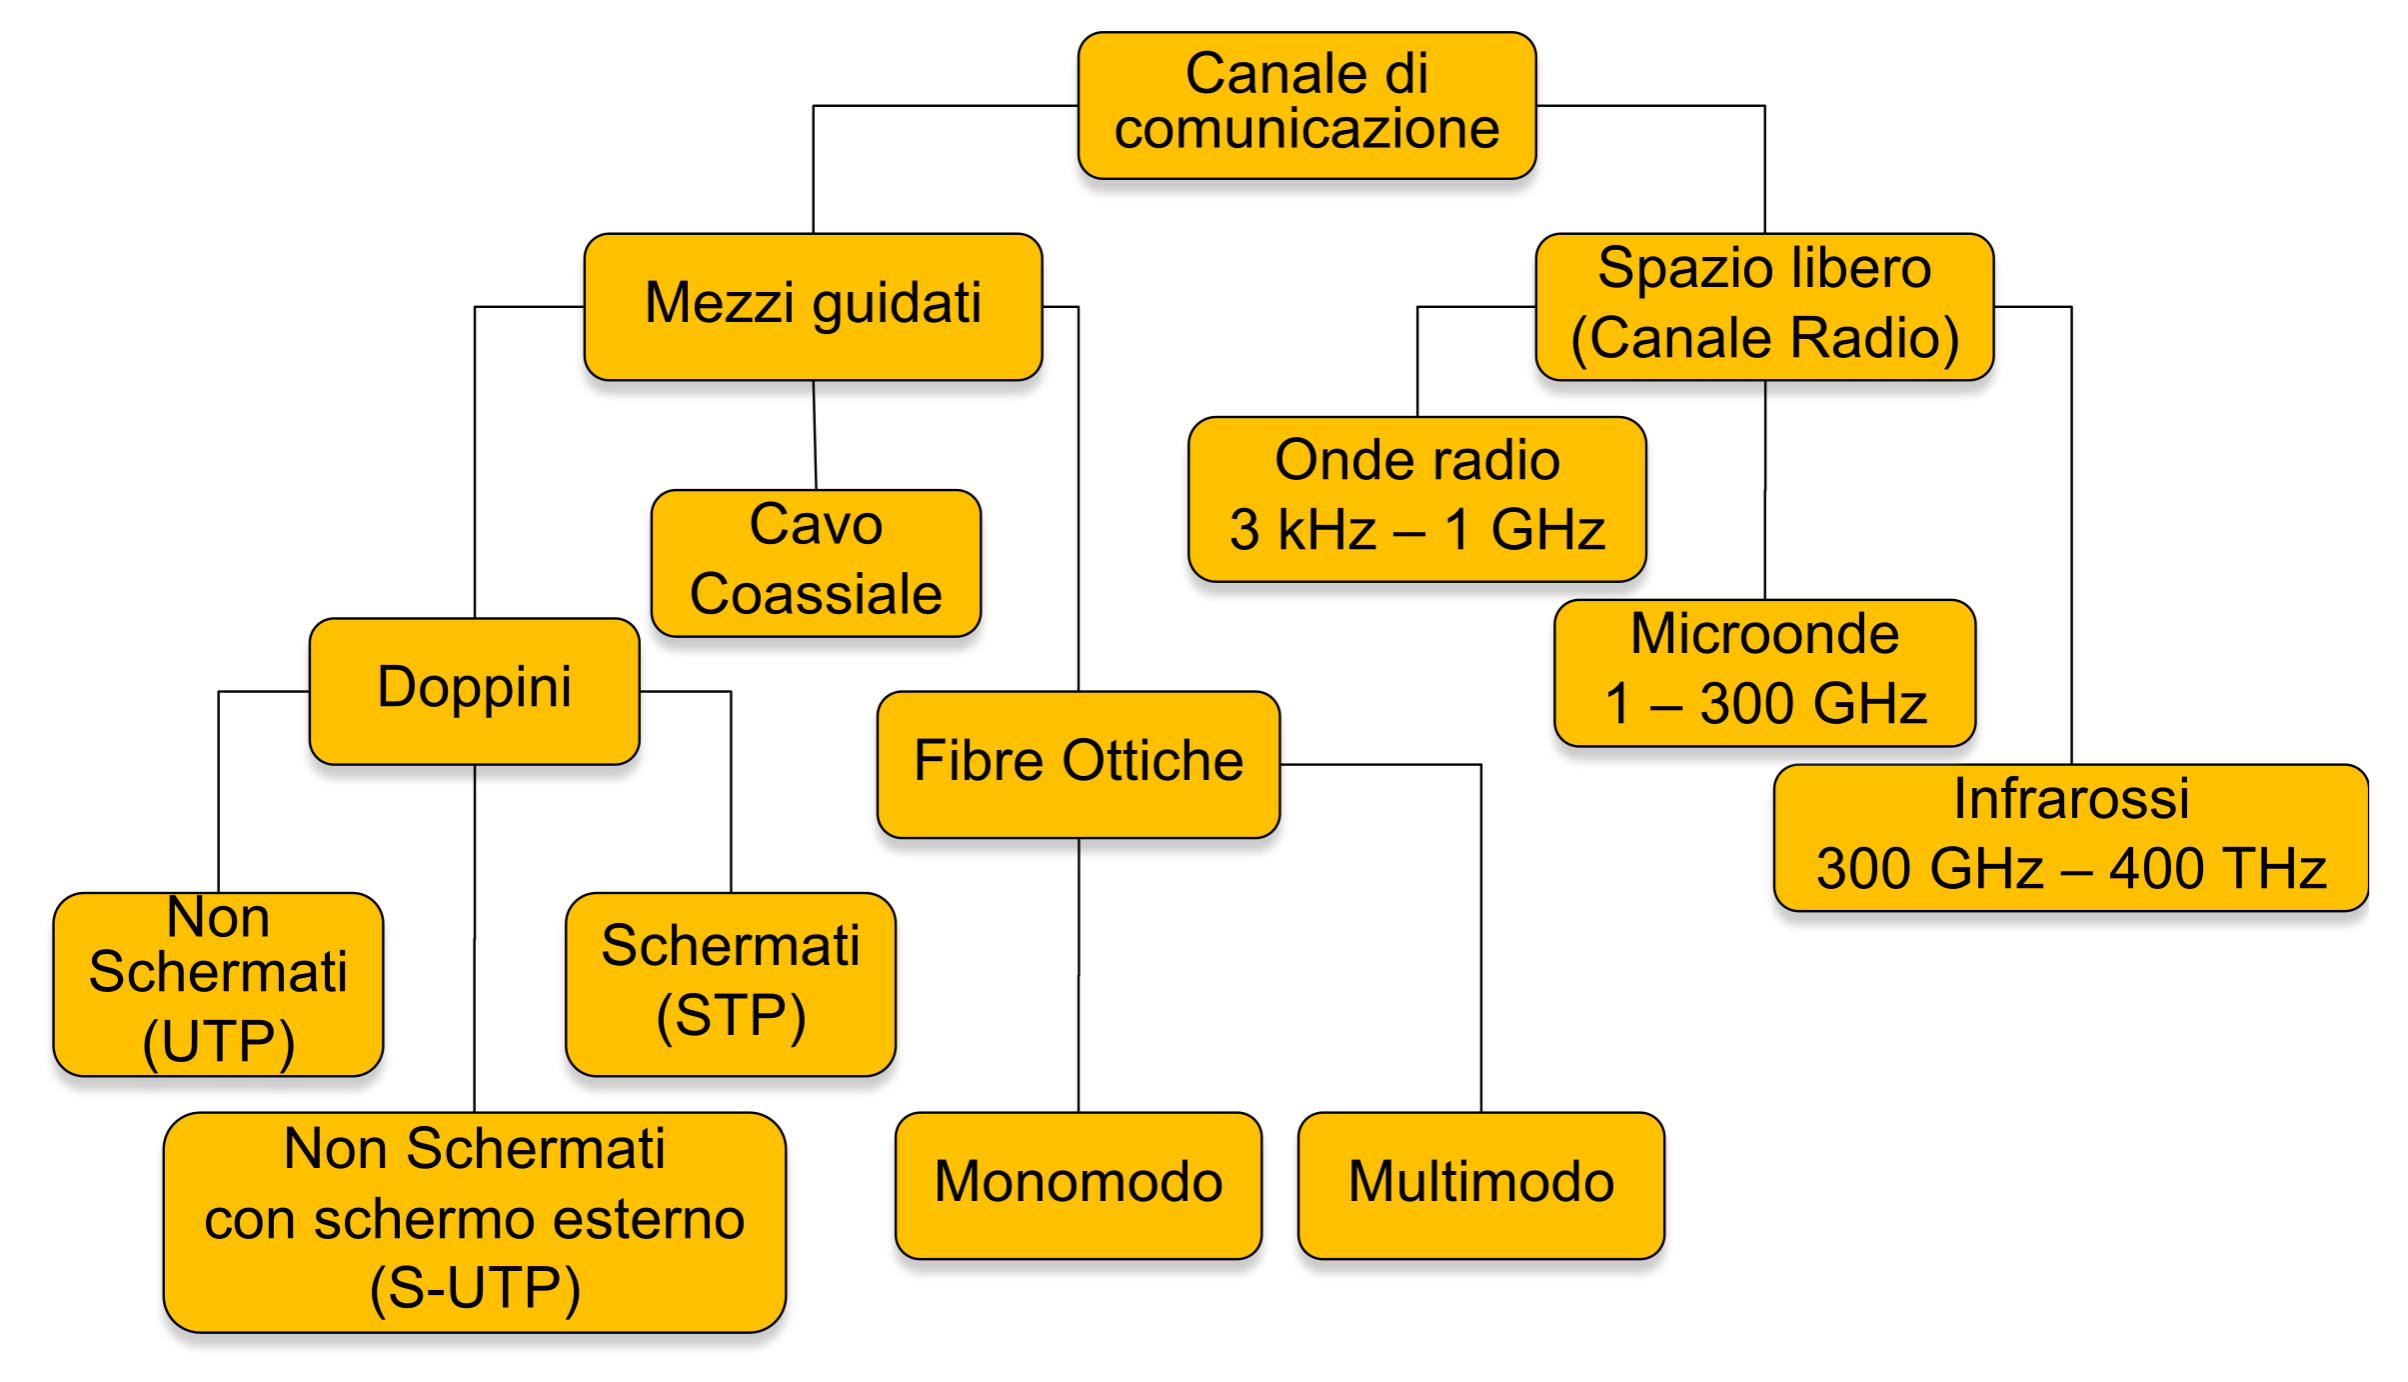
\includegraphics[width=0.8\textwidth]{images/canali_comunicazione}
    \caption{Tipi di canali di comunicazione}
    \label{fig:canali_comunicazione}
\end{figure}
\newpage
\section{Reti di telecomunicazioni - basi}
\subsection{Commutazione di circuito e commutazione di pacchetto}
\paragraph{Commutazione di circuito}
Si usava negli anni 20 del 900, quando chiamavo qualcuno inserivo il numero e nella centrale c’era qualcuno che fisicamente connetteva il mio cavo con quello a cui corrisponde il numero che ho digitato, rendendo il mezzo di comunicazione tra le due persone lo stesso cavo.
\paragraph{Commutazione di pacchetto} 
l'informazione viene impacchettata e divisa in unità, questo vuol dire che ci saranno dei ritardi dovuti a quest'impacchettamento. Le informazioni riguardanti il pacchetto stesso sono contenute nell'header, mentre nel payload c'è l'informazione, i dati che voglio trasportare. 
i nodi intermedi decidono come gestire il trasporto(commutazione) di tali pacchetti leggendo il contenuto dell’header. l’operatore ha un miglior uso di risorse.
un problema è che arrivano più pacchetti allo stesso nodo e devono attendere la commutazione del nodo che è arrivato prima.

\begin{figure}[h!]
    \centering
    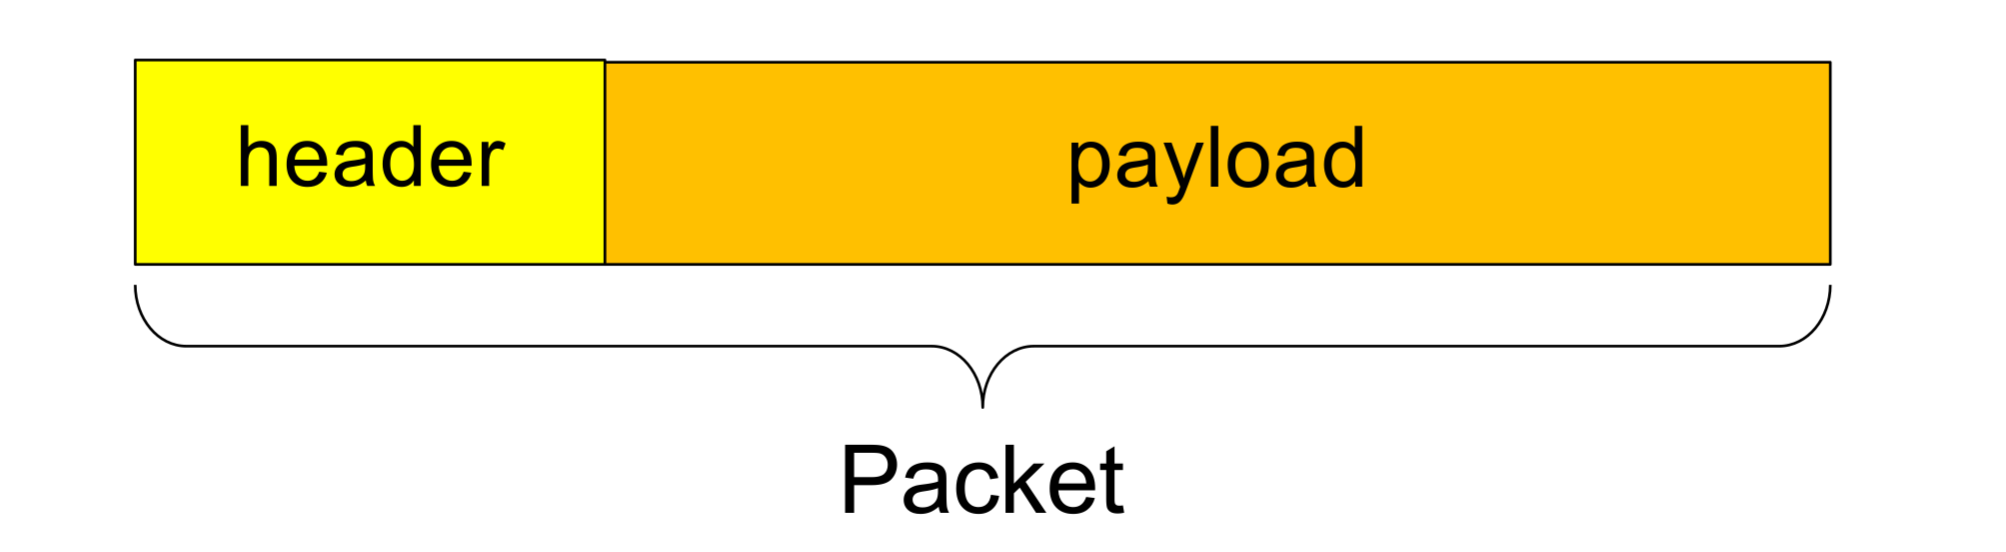
\includegraphics[width=0.7\textwidth]{images/pacchetto_generico.png}
    \caption{Commutazione di pacchetto}
    \label{fig:commutazione_pacchetto}
\end{figure}

Due tipi di commutazione di pacchetto: 
\begin{itemize}
    \item Datagram: ogni pacchetto, che prende il nome di datagramma, contiene nell’header le informazioni del mittente e destinatario. i nodi decidono la strada che deve fare il pacchetto(routing), questo viene fatto
    \item Virtual circuit: la comunicazione avviene in 3 fasi (setup, data
exchange, teardown) e l'instradamento è effettuato solo durante il setup.
Pertanto tutti i pacchetti vengono instradati lungo lo stesso percorso
(circuito), ma i nodi intermedi non devono ogni volta rieffettuare il routing,
ma solo lo switching (inoltrare il pacchetto dall'ingresso all'uscita corretta).
\end{itemize}
\newpage
\subsection{Ritardo end-to-end}
Il ritardo end-to-end è il tempo che intercorre tra l'invio di un pacchetto da parte del mittente e la ricezione dello stesso pacchetto da parte del destinatario. Questo ritardo è influenzato da diversi fattori, tra cui il tipo di rete, la distanza tra i nodi, la congestione della rete e le caratteristiche dei nodi stessi. 

Il ritardo nell'invio di un'informazione da mittente a destinatario ha più componenti:
    \begin{description}
        \item[Ritardo di trasmissione:] è il tempo necessario a inviare i bit sul mezzo, $T_f = \frac{L}{C}$, ad esempio il ritardo per la trasmissione di 1000 bit (informazione) su un cavo (canale) da 1 Gbit, $T_f = \frac{1000}{10^9}$, dove $L$ è la lunghezza in bit dell'informazione, $C$ è la frequenza di cifra.

        \item[Ritardo di propagazione:] è il tempo impiegato dai dati per attraversare la rete, tipicamente è il tempo che impiegano le onde elettromagnetiche a viaggiare in un mezzo di una certa lunghezza: $t = \frac{d}{v}$, dove $v$ è la velocità di propagazione (velocità della luce) e $d$ è la distanza considerata.

        \item[Ritardo di elaborazione:] $T_p$, è il tempo necessario all'elaborazione di un pacchetto in un nodo, dipende dalla velocità di calcolo dei processori.

        \item[Ritardo in accodamento:] $T_q$, tempo di attesa in coda nel buffer di ricezione e dipende dal traffico generato da tutti i flussi che attraversano il nodo in considerazione, è quello più difficile da prevedere e calcolare.
    \end{description}
    \begin{figure}[h!]
        \centering
        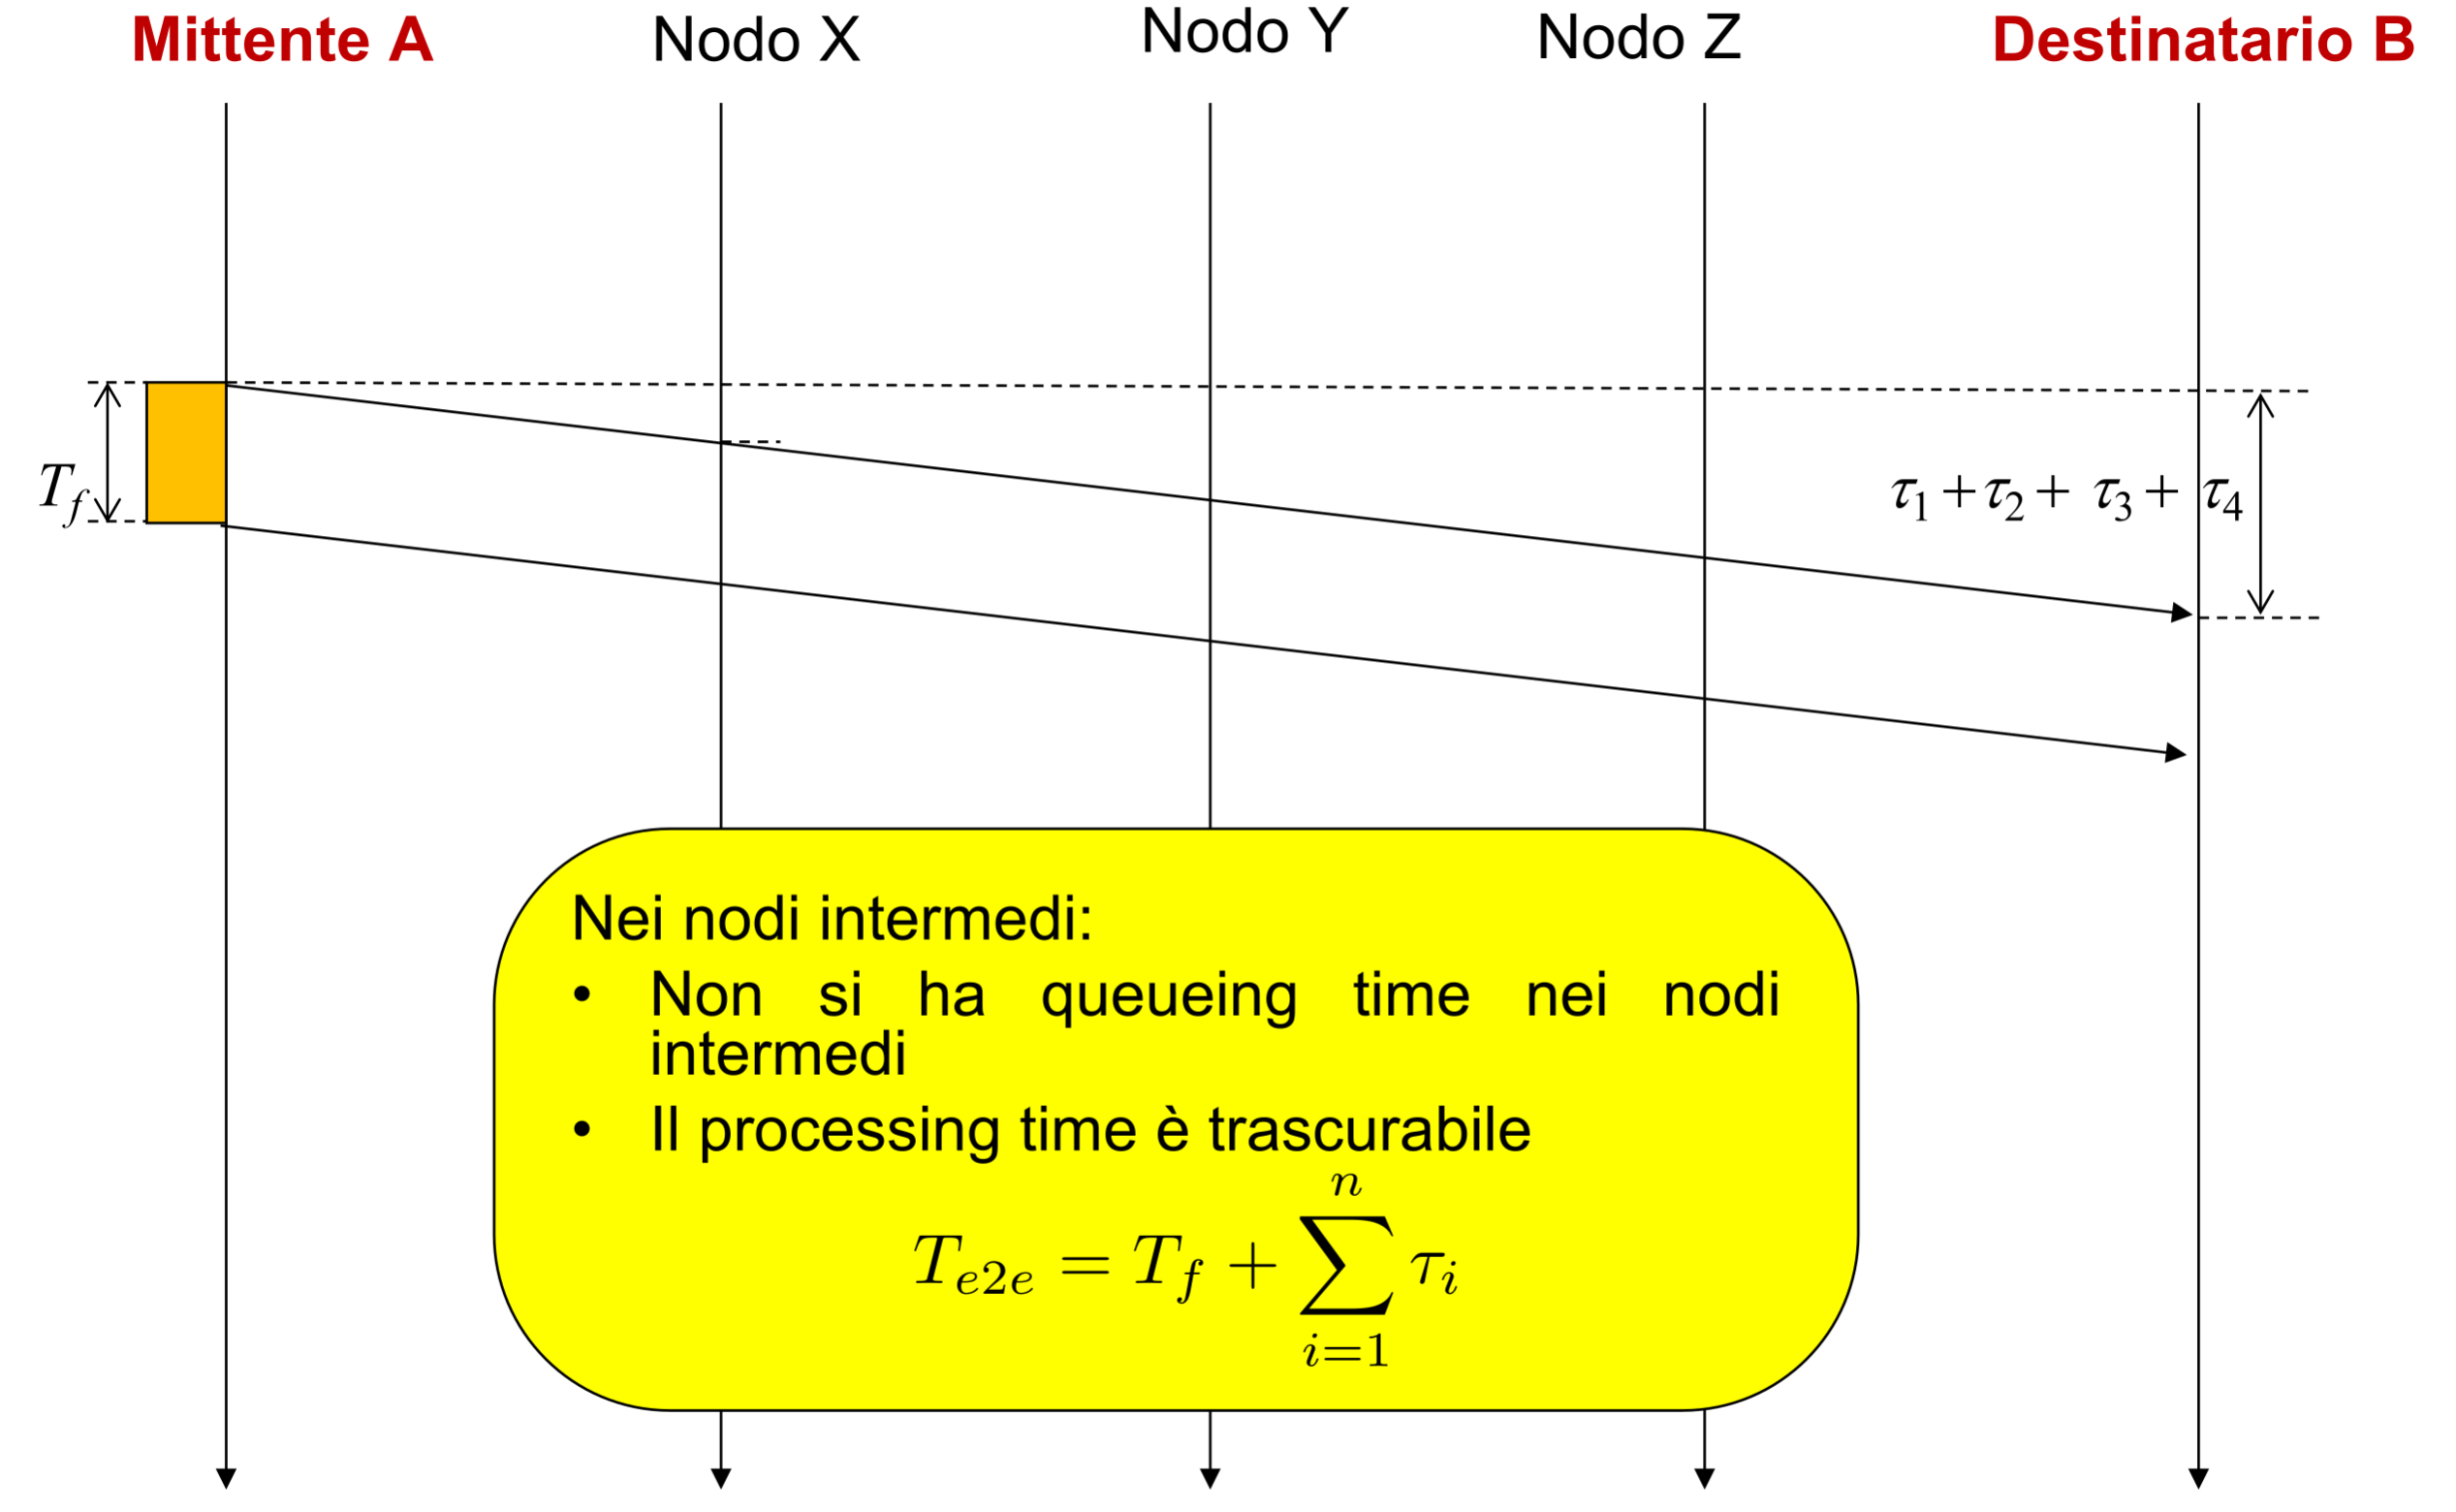
\includegraphics[width=1\textwidth]{images/e2e_circuit_switching.png}
        \caption{Ritardo e2e circuit switching: sommo i ritardi dovuti al mezzo(ritardo di trasmissione) e i ritardi dovuti alla propagazione nel mezzo}
        \label{fig:circuit_switching}
    \end{figure}
    
    
    \begin{figure}[h!]
        \centering
        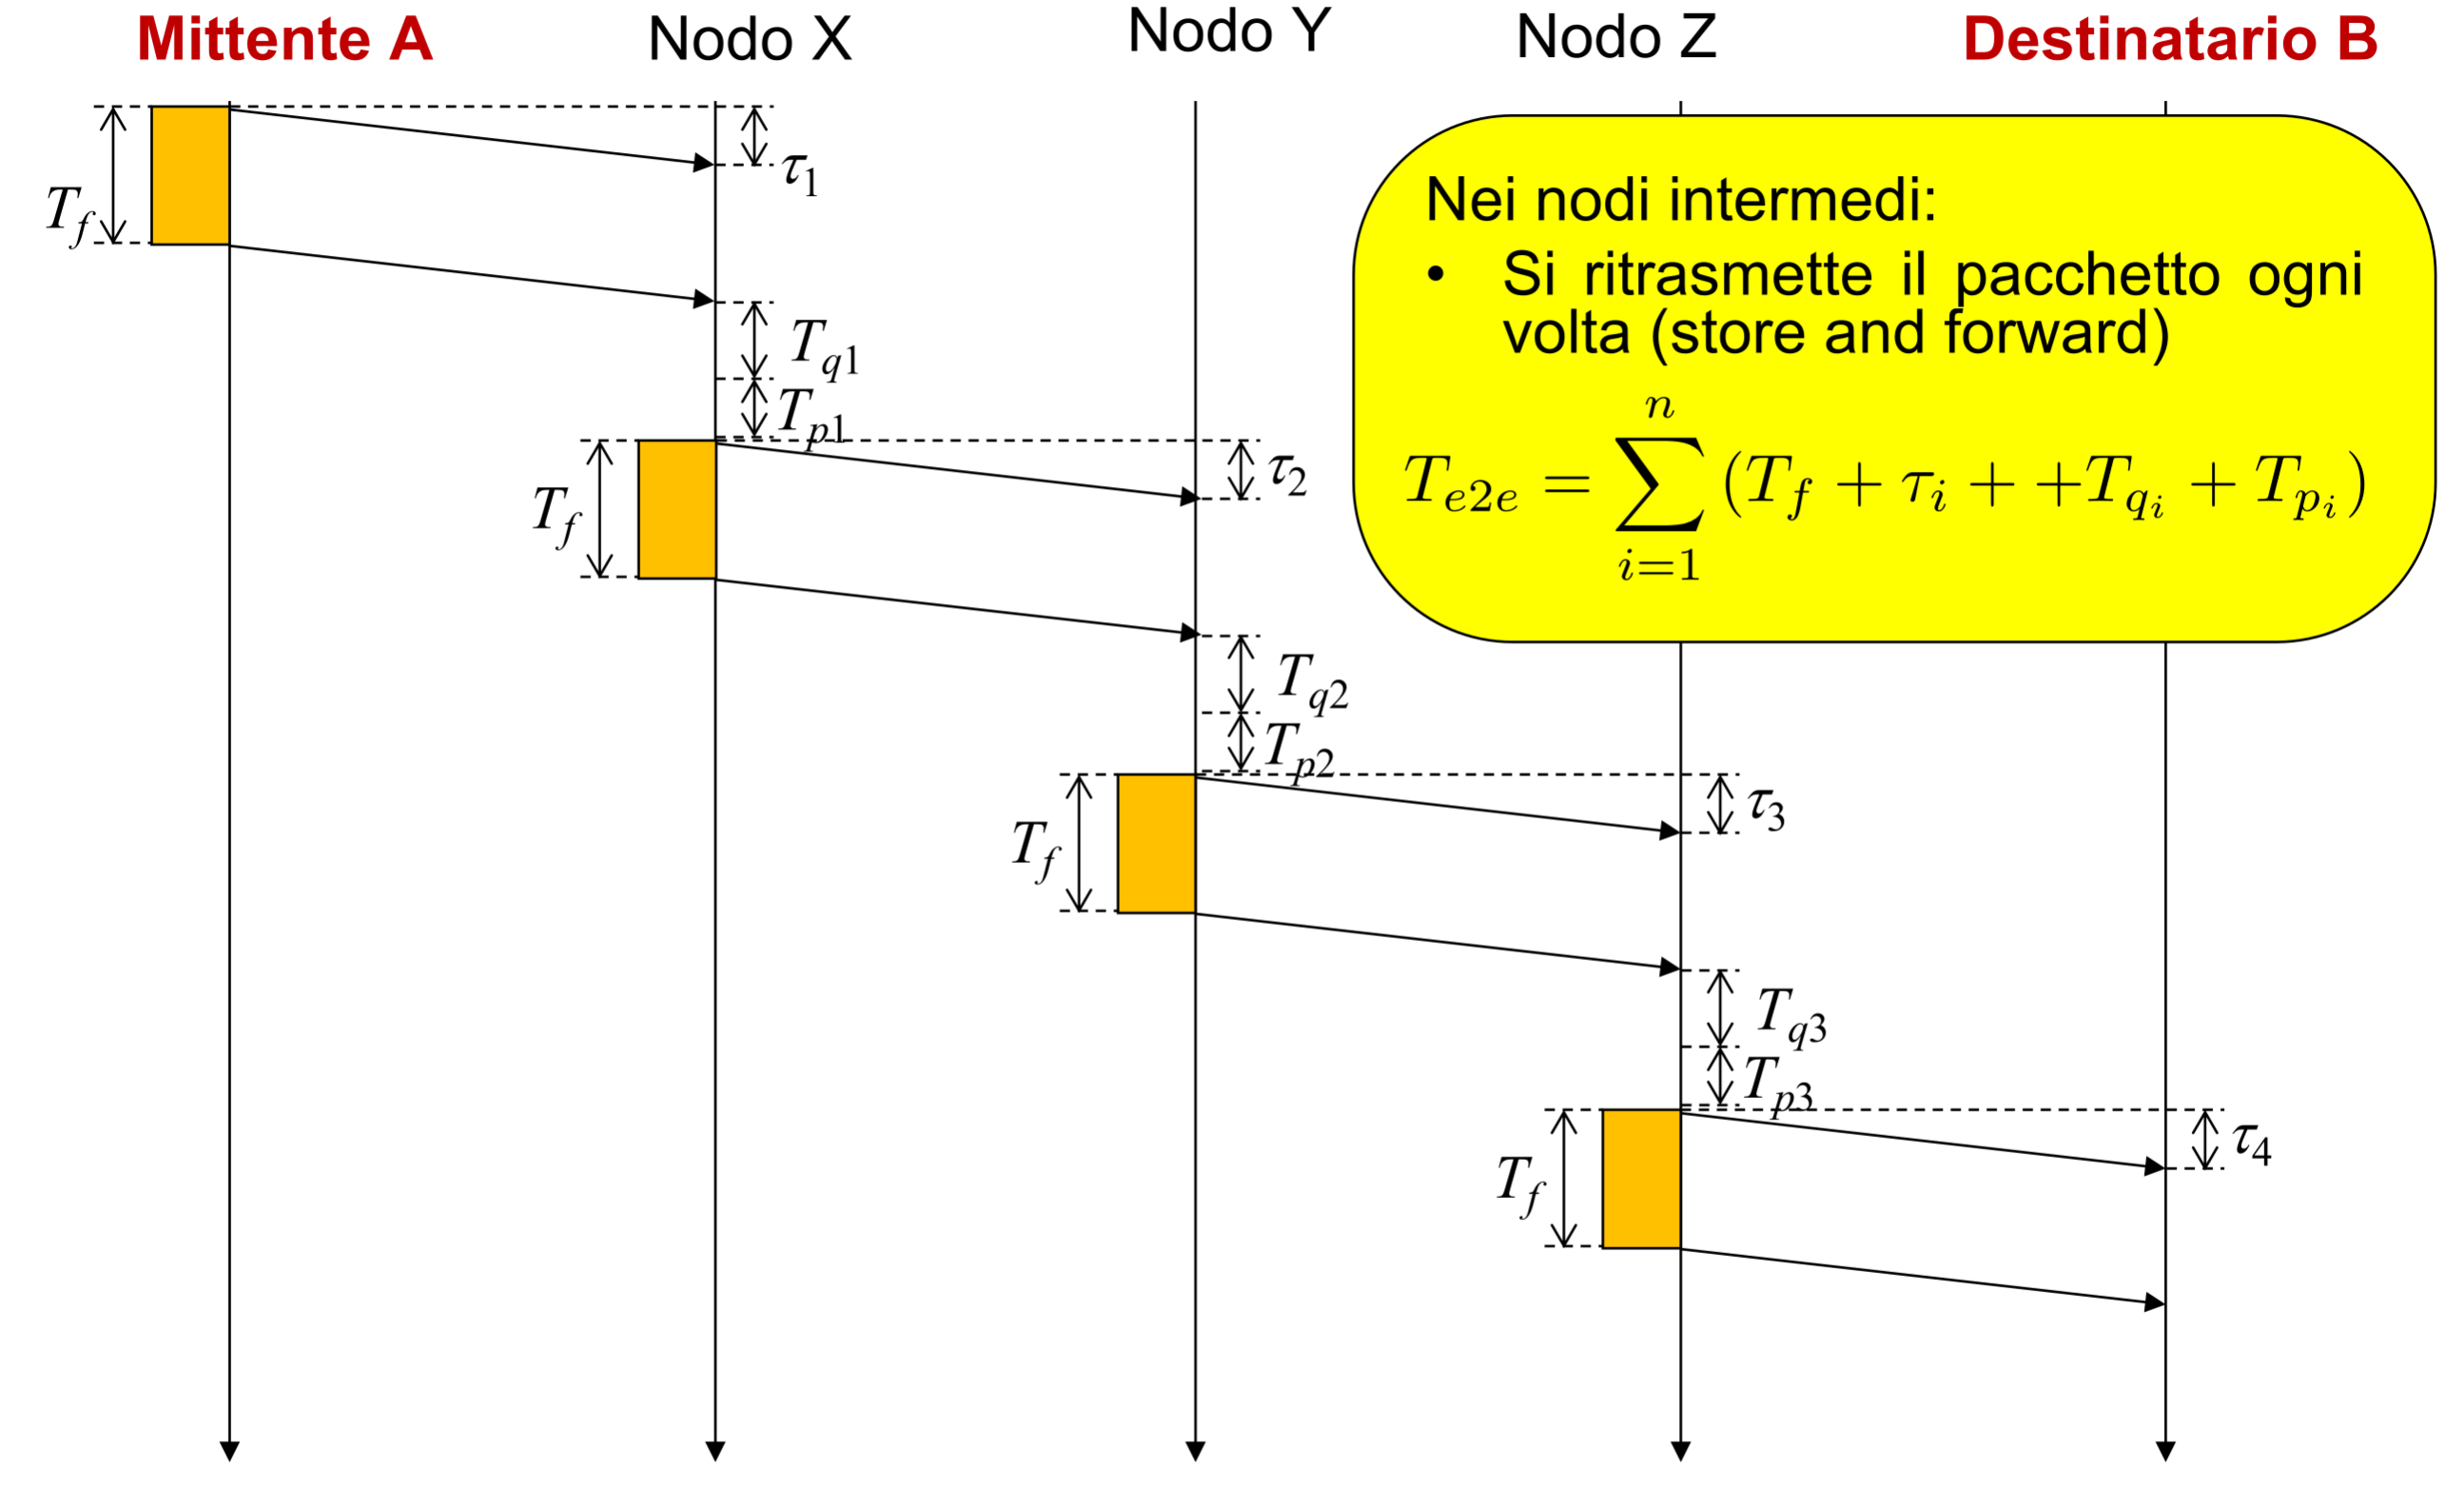
\includegraphics[width=1\textwidth]{images/e2e_packet_switching.png}
        \caption{Ritardo e2e packet switching: (sommo TUTTI i ritardi)
il packet switching ha una latenza maggiore rispetto al circuit switching}
        \label{fig:packet_switching}
    \end{figure}



%\chapter{Architetture di protocolli}
%\section{Modello ISO-OSI}
\subsection{Introduzione}
Il modello ISO-OSI è un modello di riferimento per la progettazione e l'implementazione di reti di telecomunicazioni. È stato sviluppato dall'Organizzazione Internazionale per la Standardizzazione (ISO) negli anni '80 e fornisce un framework concettuale per comprendere come i diversi protocolli e tecnologie di rete interagiscono tra loro.

ISO OSI non ha un numero fisso di livelli, è importante capire la logica dei livelli che devono comporre un modello iso osi ma il numero specifico dei livelli può variare a seconda della necessità.

\begin{enumerate}
    \item \textbf{Livello fisico}: si occupa della trasmissione dei dati attraverso il mezzo fisico (cavi, fibre ottiche, onde radio, ecc.). Definisce le caratteristiche elettriche e meccaniche dei dispositivi di rete.
    \item \textbf{Livello di collegamento dati}: gestisce la comunicazione tra i dispositivi sulla stessa rete locale. Si occupa della rilevazione e correzione degli errori, del controllo del flusso e dell'indirizzamento fisico (MAC).
    \item \textbf{Livello di rete}: si occupa dell'instradamento dei pacchetti tra reti diverse. Utilizza indirizzi logici (come gli indirizzi IP) per identificare i dispositivi sulla rete e determina il percorso migliore per inviare i dati.
    \item \textbf{Livello di trasporto}: garantisce la consegna affidabile dei dati tra i dispositivi. Si occupa della segmentazione dei dati, del controllo degli errori e del controllo del flusso. I protocolli TCP e UDP.
        \begin{multicols}{2}
            \begin{itemize}
                \item Multiplexing e demultiplexing
                \item Indirizzamento delle unità dei dati (SAP)
                \item Controllo di flusso end-to-end 
                \item Segmentazione e riassemblaggio delle unità dati
                \item Controllo errori end-to-end
            \end{itemize}
        \end{multicols}
    \item \textbf{Livello di sessione}: gestisce le sessioni di comunicazione tra i dispositivi. Si occupa dell'apertura, della chiusura e del mantenimento delle sessioni, nonché della sincronizzazione dei dati.
    \item \textbf{Livello di presentazione}: si occupa della formattazione e della codifica dei dati. Converte i dati in un formato comprensibile per il livello applicativo e gestisce la compressione e la crittografia dei dati.
    \item \textbf{Livello applicativo}: è il livello più alto del modello e fornisce agli utenti finali le interfacce per l'accesso al servizio. Esempio: posta elettronica, messaggistica istantanea. 
\end{enumerate}

\begin{figure}[h!]
    \centering
    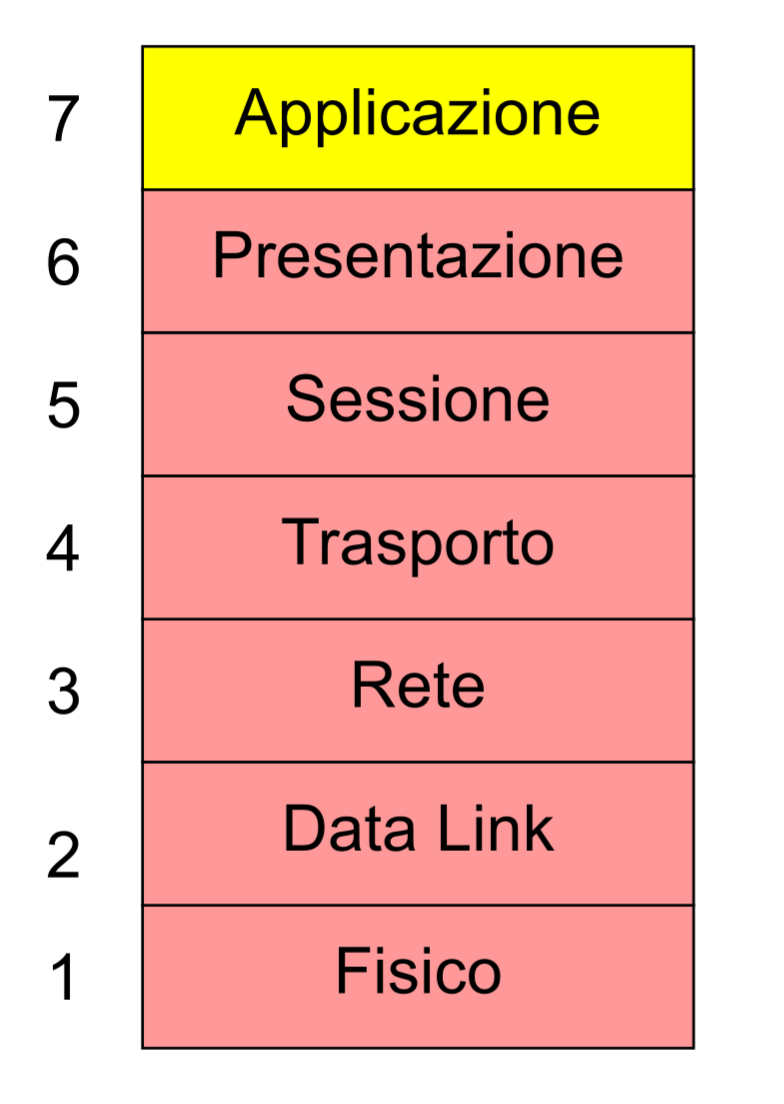
\includegraphics[width=0.45\textwidth]{images/ISO_OSI_livelli.png}
    \caption{I sette livelli del modello ISO-OSI}
    \label{fig:iso_osi_livelli}
\end{figure}

L'ISO-OSI serve a descrivere l'architettura dei protocolli, tramite il raggruppamento e la stratificazione.
vengono raggruppate tra loro le funzioni simili per logica o tecnologia.
questi gruppi vengono organizzati in modo gerarchico, quindi a strati(stratificazione). con ogni strato ci si può interfacciare trazie alle interfacce.
lo strato N è costituito da una o più entità e l'interazione tra due sistemi avviene tra strati di eguale livello e con entità pari.

Con il modello iso osi i “problemi” nella progettazione vengono divisi, rendendo la progettazione più modulare e più semplice, potendo specializzarsi su un livello specifico del modello. dividere un problema in più livelli è più conveniente. 
\subsubsection{Entità e pacchetti}
Ogni livello ha un'entità, queste elaborano i pacchetti, un pacchetto(PDU: protocol data unit) è composto da un header(PCI:protocol control information) e un payload(SDU: service data unit) 
\subsection{Segmentazione e riassemblaggio} 
La segmentazione è il processo di suddivisione dei dati in pacchetti più piccoli per facilitarne la trasmissione attraverso la rete. Ogni pacchetto viene inviato separatamente e può seguire percorsi diversi attraverso la rete. Il riassemblaggio è il processo inverso, in cui i pacchetti ricevuti vengono ricomposti nell'ordine corretto per ricostruire i dati originali.
(dall’alto verso il basso(segmentazione) vengono aggiunti gli header ai pacchetti; dal basso verso l’alto(riassemblaggio) vengono rimossi, quindi utilizzati, gli header dei pacchetti)
\subsubsection{Incapsulamento e decapsulamento}
Dall'alto verso il basso: trasmissione $\rightarrow$ da tenere a mente che il livello più basso c’è il livello fisico, mentre il livello più alto è quello a cui tipicamente ci interfacciamo(applicazione del telefono ad esempio, whatsapp)
quando trasmetto quindi faccio encapsulation, ossia aggiungo informazioni utili alla trasmissione del payload. questo perchè tra un livello è l’altro potrei avere la necessità di dover dividere il pacchetto in altri pacchetti, perciò va aggiunto negli header le informazioni necessarie a far riassemblare il pacchetto intero una volta finita la trasmissione.
\begin{figure}[h!]
    \centering
    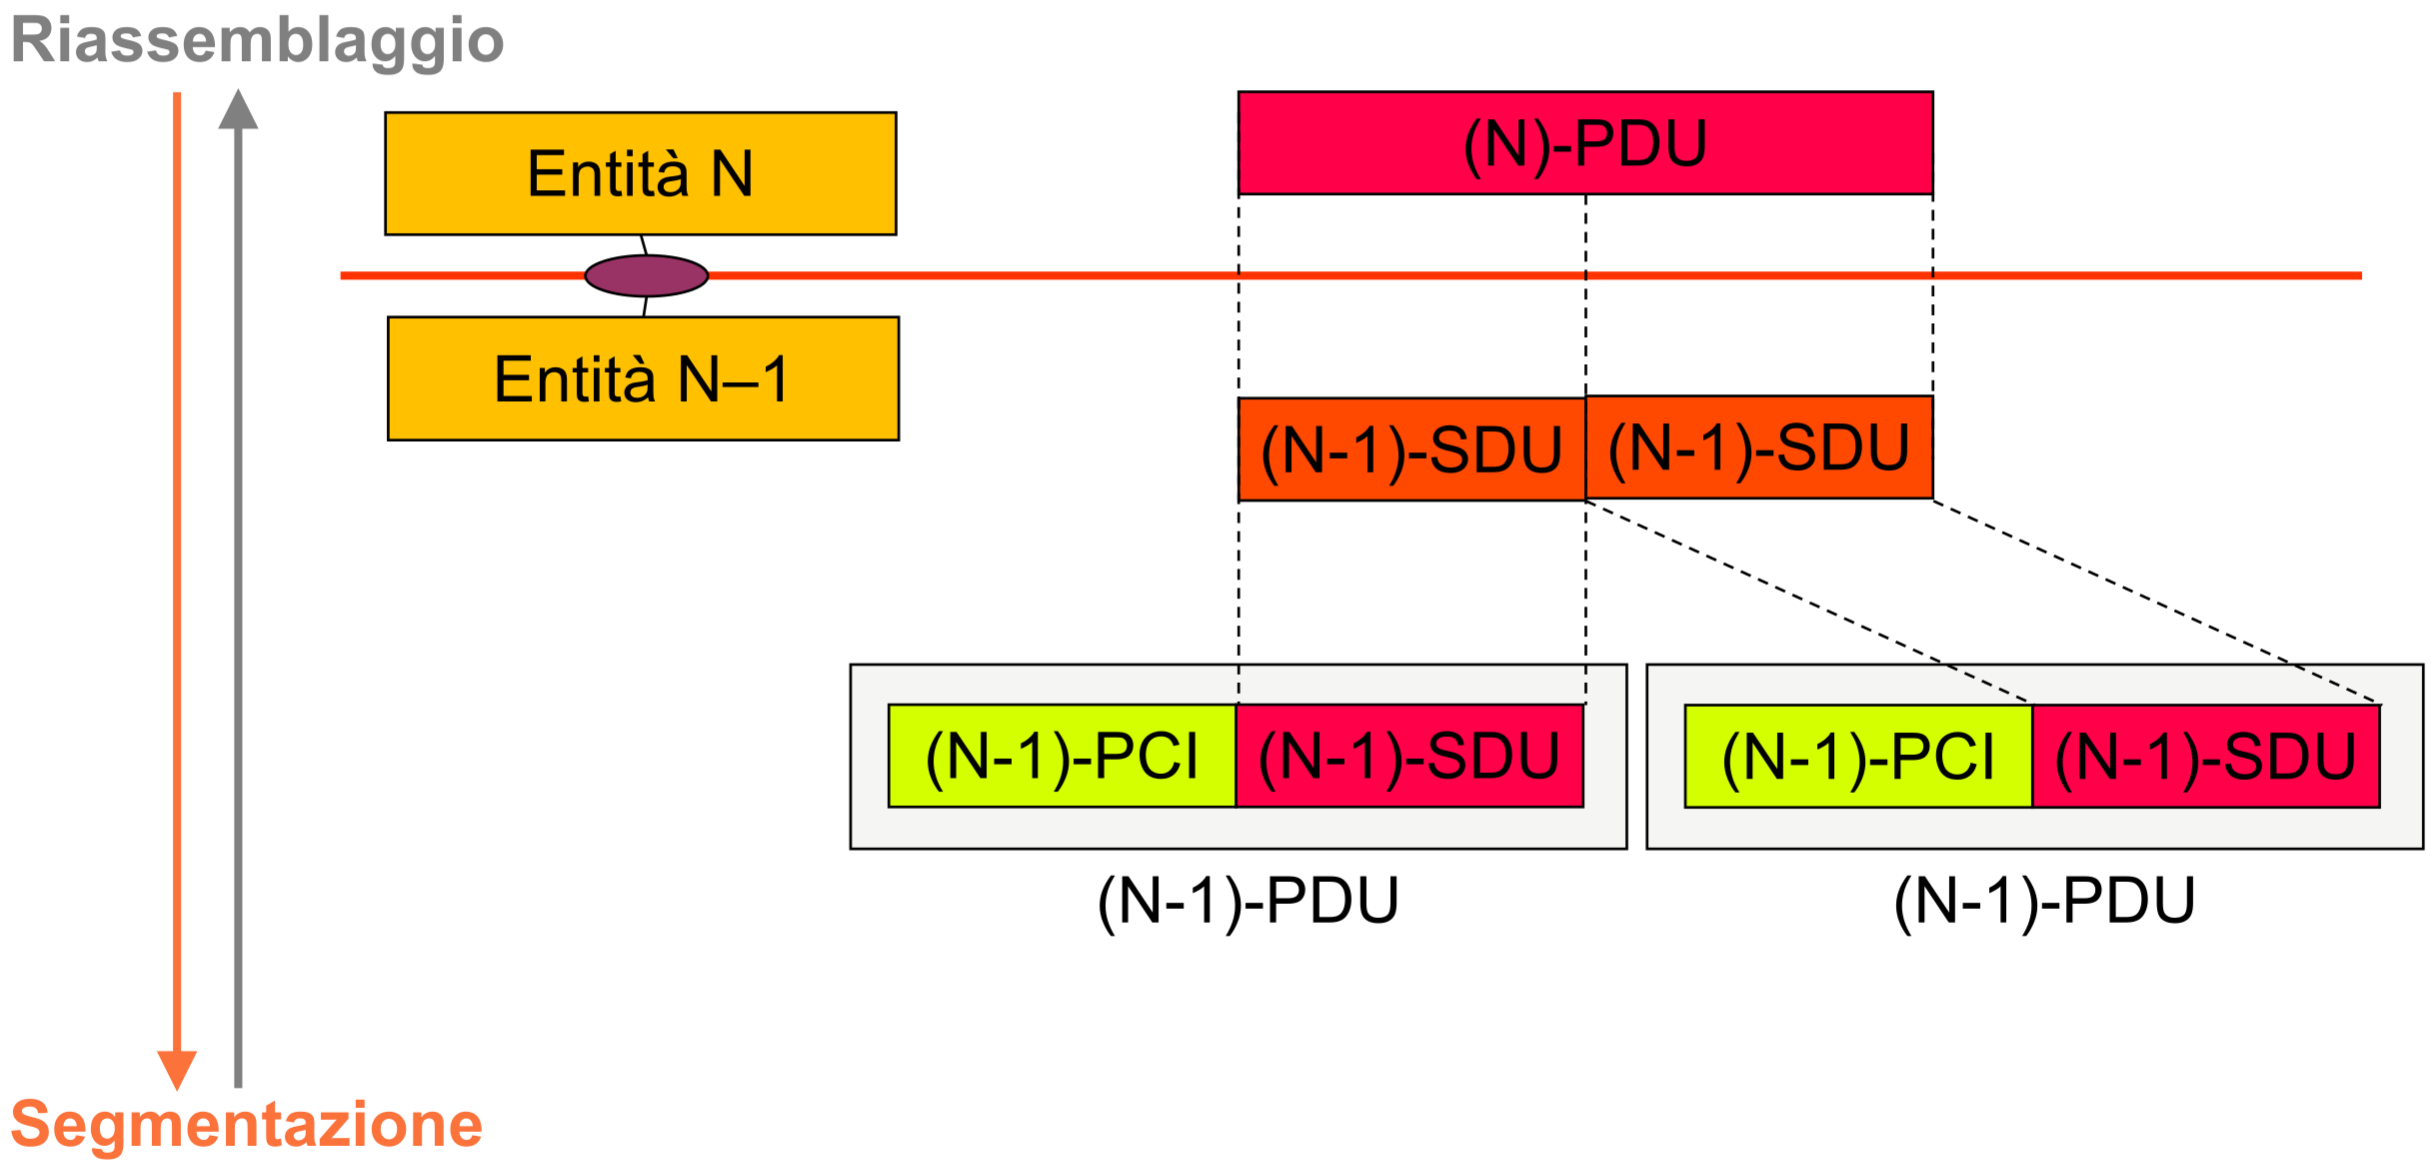
\includegraphics[width=1\textwidth]{images/ISO_OSI_incapsulamento.png}
    \caption{Pacchetti e incapsulamento/decapsulamento}
    \label{fig:pacchetti}
\end{figure}



\newpage
\section{Modello ibrido}
Il modello ibrido è un modello di rete che combina elementi del modello ISO-OSI e del modello TCP/IP. È stato sviluppato per affrontare le limitazioni del modello ISO-OSI e per adattarsi meglio alle esigenze delle reti moderne.
Il modello ibrido è composto da cinque livelli principali:
\begin{enumerate}
    \item \textbf{Livello fisico}: simile al livello fisico del modello ISO-OSI, si occupa della trasmissione dei dati attraverso il mezzo fisico.
    \item \textbf{Livello di collegamento dati}: gestisce la comunicazione tra i dispositivi sulla stessa rete locale e include funzioni di rilevamento degli errori e controllo del flusso.
    \item \textbf{Livello di rete}: simile al livello di rete del modello ISO-OSI, si occupa dell'instradamento dei pacchetti tra reti diverse.
    \item \textbf{Livello di trasporto}: fornisce servizi di trasporto affidabili e non affidabili, come TCP e UDP.
    \item \textbf{Livello applicativo}: fornisce servizi di rete agli utenti finali e include protocolli come HTTP, FTP e SMTP.
    \end{enumerate}

    \begin{figure}[h!]
    \centering
    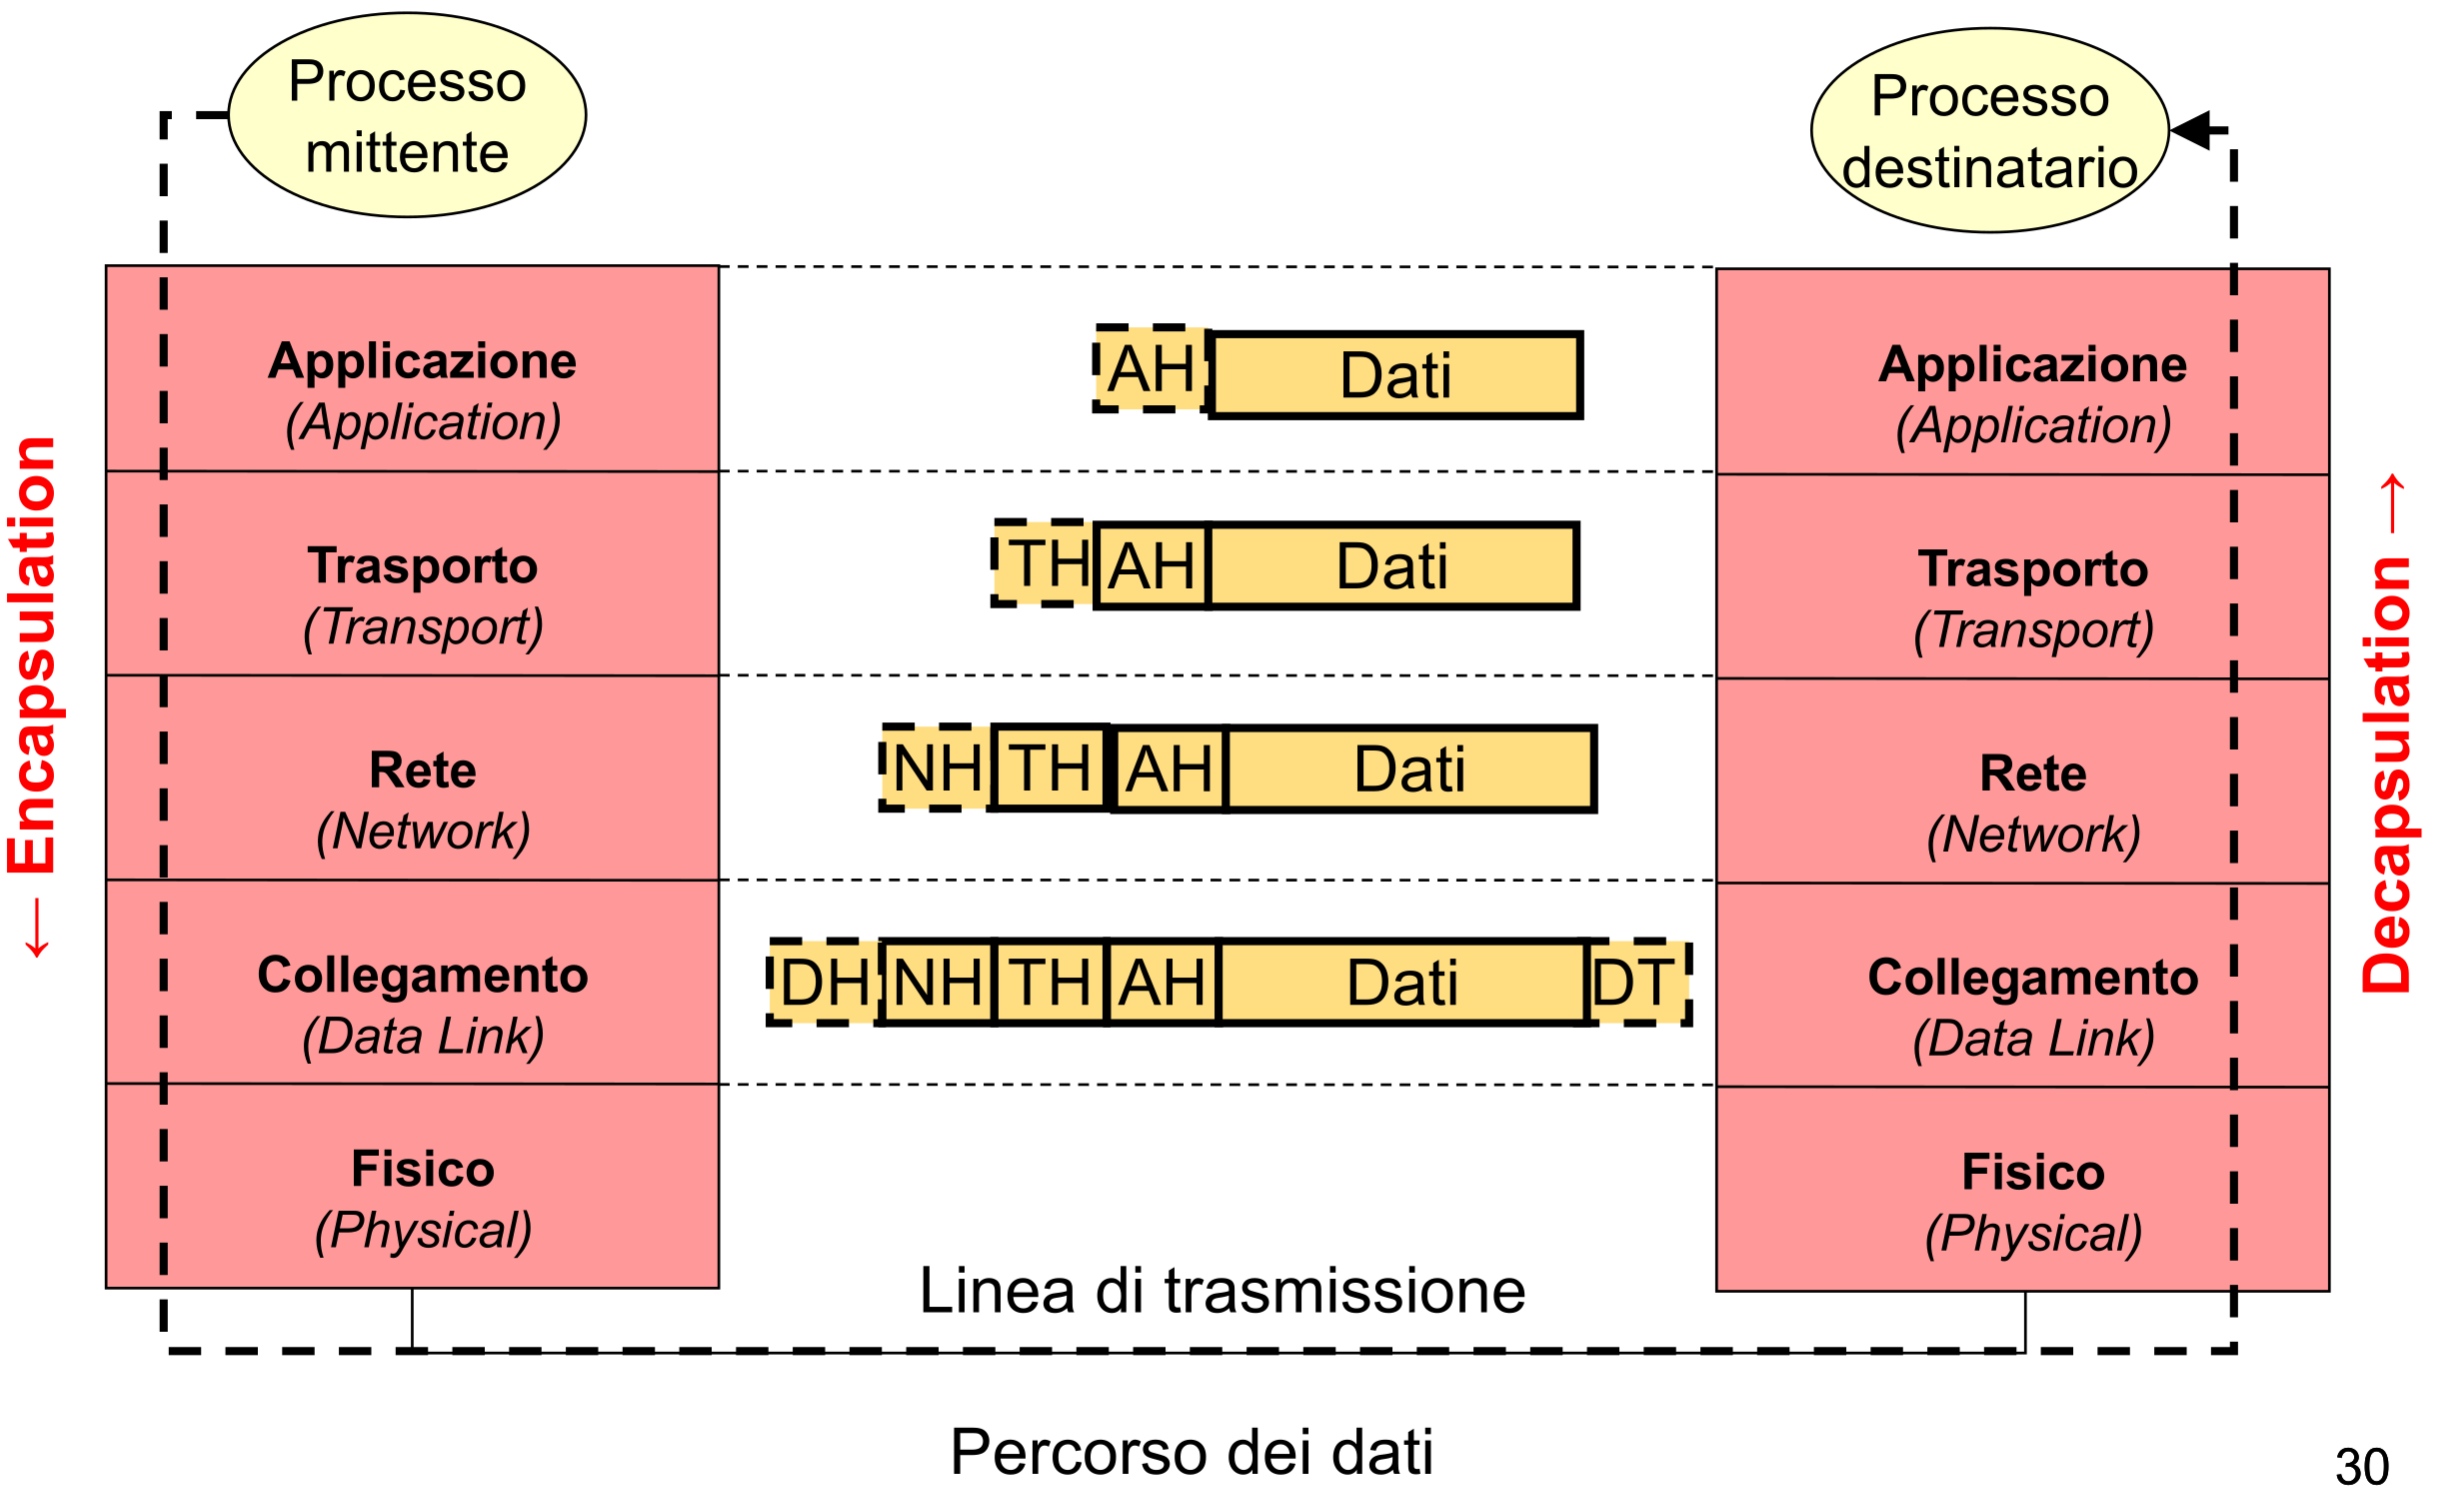
\includegraphics[width=1.2\textwidth]{images/enc_dec_ibrido.png}
    \caption{Incapsulamento e decapsulamento dei dati nel modello ibrido}
    \label{fig:modello_ibrido_enc_decapsulamento}
\end{figure}

\subsection{Enc/decapsulation dati nel modello ibrido}
Durante l'encapsulation vengono ad ogni livello aggiunti degli header(AH = application heder, TH = transport header, NH = network header ecc), durante la decapsulation vengono spacchettati grazie agli header precedentemente aggiunti ad ogni livello
l'unico livello che aggiunge oltre ad un header anche una coda(tail) è il “data link” , “collegamento”, questo perchè vuole verificare la correttezza del pacchetto, tramite tecniche che vedrò avanti(algoritmi di controllo, non esiste un metodo che garantisce che il pacchetto che sia 100 corretto.% corretto, come l’evenienza in cui dopo la verifica mi risulta corretto ma poi si scopre incorretto, falso positivo).

\subsection{Comunicazione tra sistemi}
i livelli rete, data link e fisico si occupano del trasporto dell’informazione tra il sistema a ed il sistema b. questo può avvenire tramite il nodi, intermediari, x e y, oppure in modo diretto.
il datalink presuppone un collegamento diretto ed è fondamentale che riceva informazion dal livello fisico poichè gestisce il passaggio di info tra un mezzo fisico e l’altro. al pacchetto viene aggiunto tramite il datalink un header che gestisce il passaggio tra a e x, quindi utilizzando un indirizzo locale. a livello di datalink inoltre viene viene verificato che il pacchetto sia inviato correttamente(evitando il loop: deadlog). dopo aver verificato la correttezza del pacchetto, a livello di rete ci si assicura che il pacchetto ricevuto sia arrivato a destinazione. nel caso specifico il pacchetto che arriva al livello di rete del nodo x viene spedito al nodo successivo poichè il livello di rete del nodo x capisce che non era lui il destinatario, tramite la lettura dell’header inserito dal sistema a inizialmente. 
tra un nodo e l’altro è possibile usare tecnologie differenti, cavo, wireless ecc, livello fisico

se al livello b arriva un pacchetto errato allora viene reinviato il pacchetto da b ad a così da far capire ad a che deve reinviare il pacchetto, latenza.
posso inserire un timer oltre il quale si interrompe la trasmissione, per evitare loop o perdite di informazioni.

\begin{figure}[h!]
    \centering
    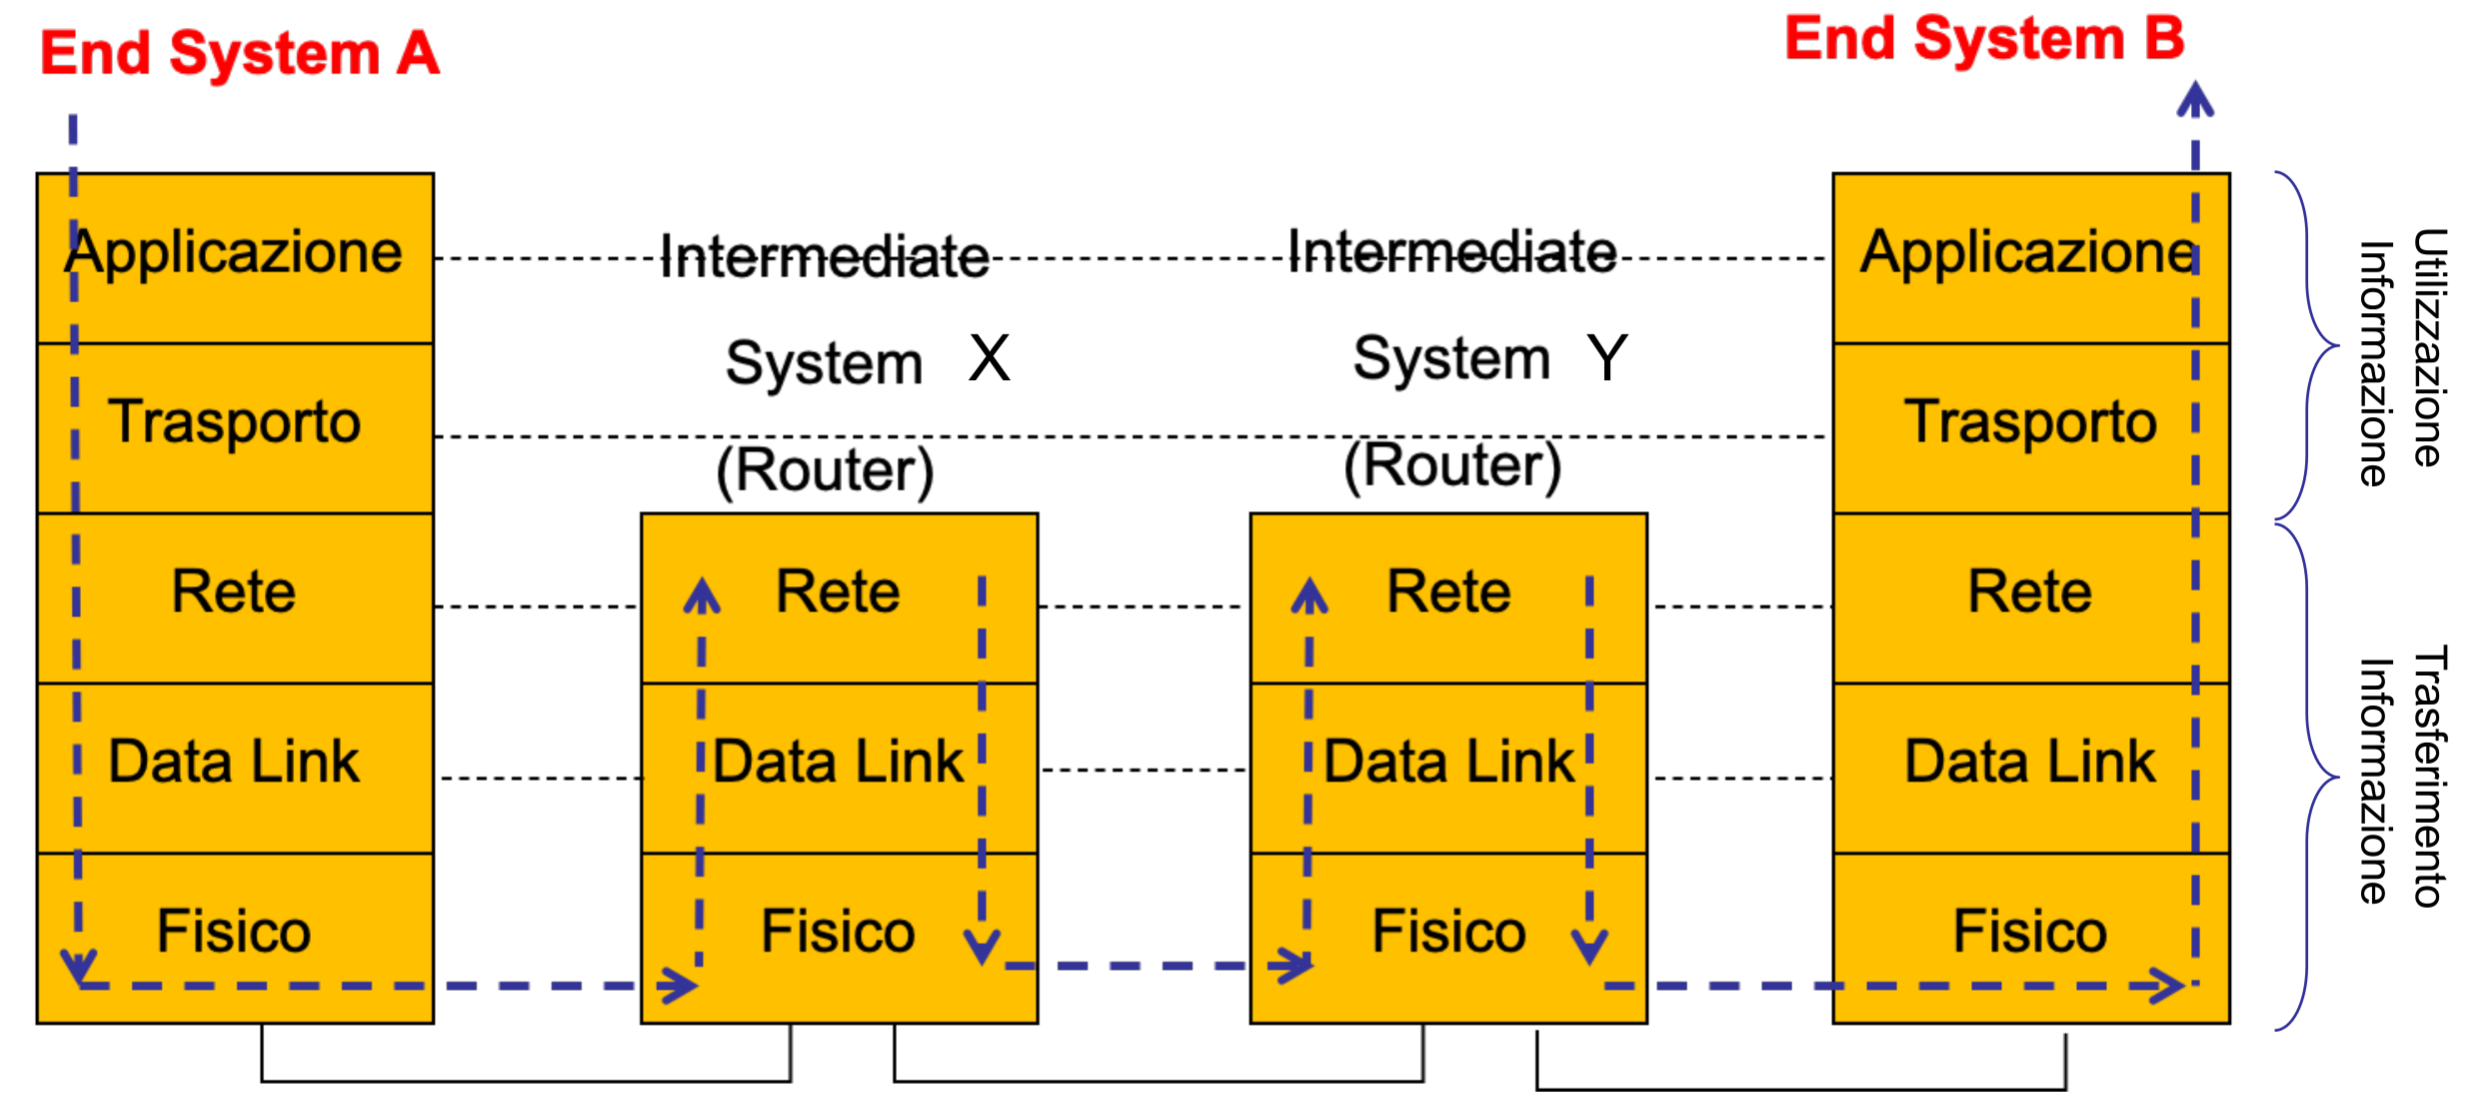
\includegraphics[width=1\textwidth]{images/comunicazione_ibrido.png}
    \caption{Comunicazione tra sistemi nel modello ibrido}
    \label{fig:comunicazione_sistemi_ibrido}
\end{figure}


    \newpage
\section{Modello TCP/IP}
Il modello tcp/ip nasce a 4 livelli(negli anni 70), il livelllo di rete si chiama internet, poichè a quel livello si usa il protocollo ip(internet protocol).

Il suo nome è dovuto dai due protocolli principali che lo compongono: TCP (Transmission Control Protocol) e IP (Internet Protocol).

I livelli del modello TCP/IP:
\begin{enumerate}
    \item \textbf{Livello di accesso alla rete}: corrisponde ai livelli DataLink e Fisico del modello ISO-OSI.
    \item \textbf{Livello Internet}: si occupa dell'instradamento dei pacchetti tra reti diverse. Utilizza indirizzi logici (come gli indirizzi IP) per identificare i dispositivi sulla rete e determina il percorso migliore per inviare i dati.
    A consentire lo scambio di informazioni tra nodie della rete è l'ICMP, l' Internet Control Message Protocol. Al livello di rete sono presenti anche protocolli di routing. 
    Importante: non prevede l'interlavoro tra protocolli di rete
diversi, ma necessariamente tutti i nodi devono
utilizzare IP.
    \item \textbf{Livello di trasporto}: fornisce servizi di trasporto affidabili(TCP) e non affidabili(UDP), come TCP e UDP. Si occupa della segmentazione dei dati, del controllo degli errori e del controllo del flusso.
    \item \textbf{Livello applicativo}: Come ISO OSI e ibrido
\end{enumerate}

\begin{figure}[h!]
    \centering
    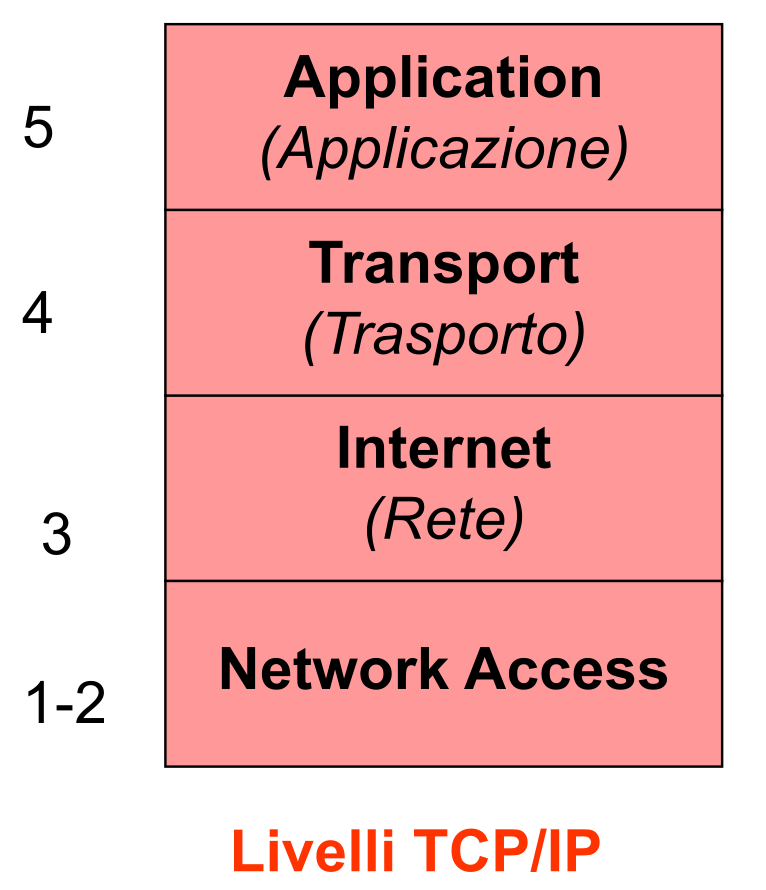
\includegraphics[width=0.5\textwidth]{images/modello_TCP_IP.png}
    \caption{I livelli del modello TCP/IP}
    \label{fig:tcp_ip_modello}
\end{figure}



\subsubsection{Confronto tra i modelli}
I tre modelli — ISO-OSI, TCP/IP e il modello ibrido — sono utilizzati per descrivere l’architettura delle reti di telecomunicazione, ma presentano differenze significative in termini di struttura, approccio e utilizzo pratico.

\textbf{Modello ISO-OSI}: è un modello teorico a 7 livelli, sviluppato come riferimento universale per la progettazione delle reti. Ogni livello ha funzioni ben definite e interagisce solo con i livelli adiacenti. Il modello ISO-OSI è molto dettagliato e didattico, ma non è stato adottato integralmente nelle implementazioni pratiche.

\textbf{Modello TCP/IP}: nasce dall’esperienza pratica di Internet e si compone di 4 livelli. È meno dettagliato rispetto all’ISO-OSI, ma più semplice e orientato all’implementazione. Il modello TCP/IP è diventato lo standard de facto per le reti moderne.

\textbf{Modello ibrido}: rappresenta un compromesso tra i due modelli precedenti, combinando la chiarezza concettuale dell’ISO-OSI con la semplicità e la praticità del TCP/IP. Il modello ibrido solitamente prevede 5 livelli, raggruppando alcune funzioni e adattandosi meglio alle esigenze delle reti attuali.

In sintesi, il modello ISO-OSI è utile per comprendere i principi teorici delle reti, il modello TCP/IP è quello realmente utilizzato nelle reti Internet, mentre il modello ibrido cerca di unire i vantaggi di entrambi per una maggiore flessibilità e chiarezza.

\begin{figure}[h!]
    \centering
    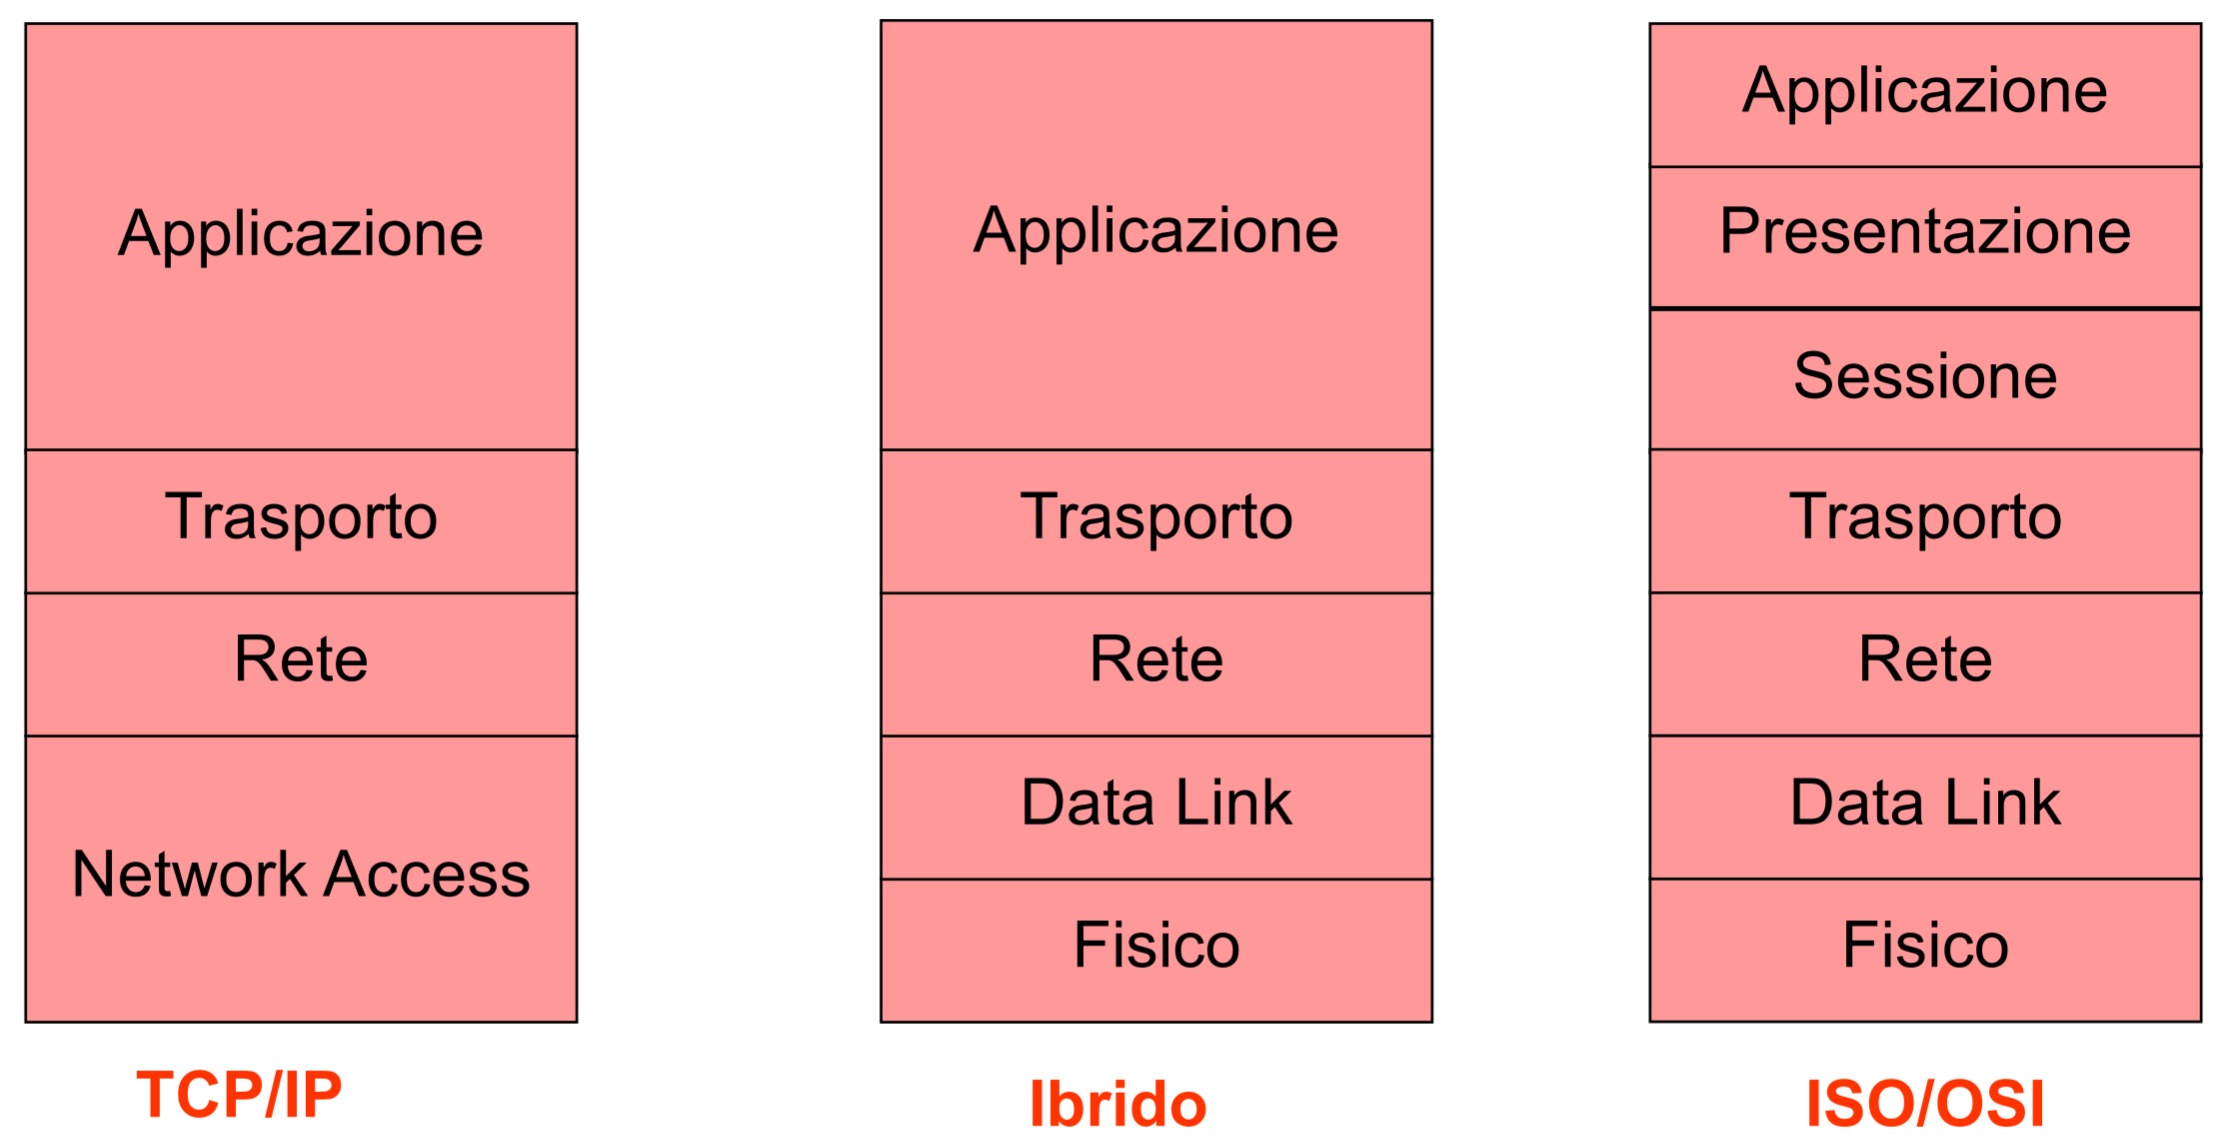
\includegraphics[width=1\textwidth]{images/confronto_stack.png}
    \caption{Confronto tra stack ISO-OSI, TCP/IP e modello ibrido}
    \label{fig:confronto_stack}
\end{figure}

%\chapter{Livello 4 trasporto TCP/UDP}
%\section{Nozioni preliminari}
UDP(Used Datagram Protocol) e TCP(Transmission Control Protocol) sono i protocolli di trasporto(livello 4) più diffusi.
Principali differenze:
\begin{itemize}
    \item TCP è orientato alla connessione, UDP no (vuol dire che non è necessario stabilire una connessione prima di inviare i dati, cosa invece necessaria con TCP)
    \item TCP è un protocollo di trasporto affidabile, UDP è non affidabile(quindi TCP garantisce che i dati arrivino a destinazione e nell'ordine corretto, mentre UDP non lo fa)
\end{itemize}

I pacchetti(PDU) TCP sono chiamati segmenti, mentre i pacchetti UDP sono chiamati datagrammi.

\paragraph{Funzioni principali UDP}
Svolge l'unico compito di incapsulare i dati dell'applicazione in un pacchetto UDP, aggiungendo le informazioni necessarie per la consegna(Multiplexing). Non fornisce alcuna garanzia di consegna o ordine dei pacchetti.
\paragraph{Funzioni principali TCP}
\begin{multicols}{2}
\begin{itemize}
    \item Controllo flusso end to end
    \item Controllo congestione end to end
    \item Ritrasmette le PDU perse o corrotte
    \item Riordina i segmenti ricevuti in ordine corretto
\end{itemize}
\end{multicols}
Il TCP numera i singoli byte che arrivano dal livello applicativo, e non i segmenti; è fondamentale poichè dal livello 3(IP) non arrivano i byte in ordine, ma i pacchetti possono arrivare in ordine sparso.

\subsection{Sock e ports}
Dei concetti fondamentali per il funzionamento di TCP e UDP sono i socket e le porte.
\begin{itemize}
    \item Socket: è un punto finale di una connessione di rete, rappresentato da:
    \begin{itemize}
        \item Indirizzo IP: identifica un host sulla rete
        \item Porta: identifica un'applicazione in esecuzione su quell'host 
    \end{itemize}
    I socket sono utilizzati per inviare e ricevere dati tra applicazioni su host diversi.
    \item Porta: è un numero che identifica un'applicazione in esecuzione su un host. Le porte sono numerate da 0 a 65535 e sono suddivise in tre categorie: well-known ports, registered ports e dynamic/private ports.
\end{itemize}
Il numero di porta è un numero a 16 bit che identifica un'applicazione in esecuzione su un host. Quando un client invia una richiesta HTTP a un server web, utilizza la porta 80 per comunicare con il server. Il server ascolta sulla porta 80 e risponde alla richiesta del client.

\begin{figure}[h!]
    \centering
    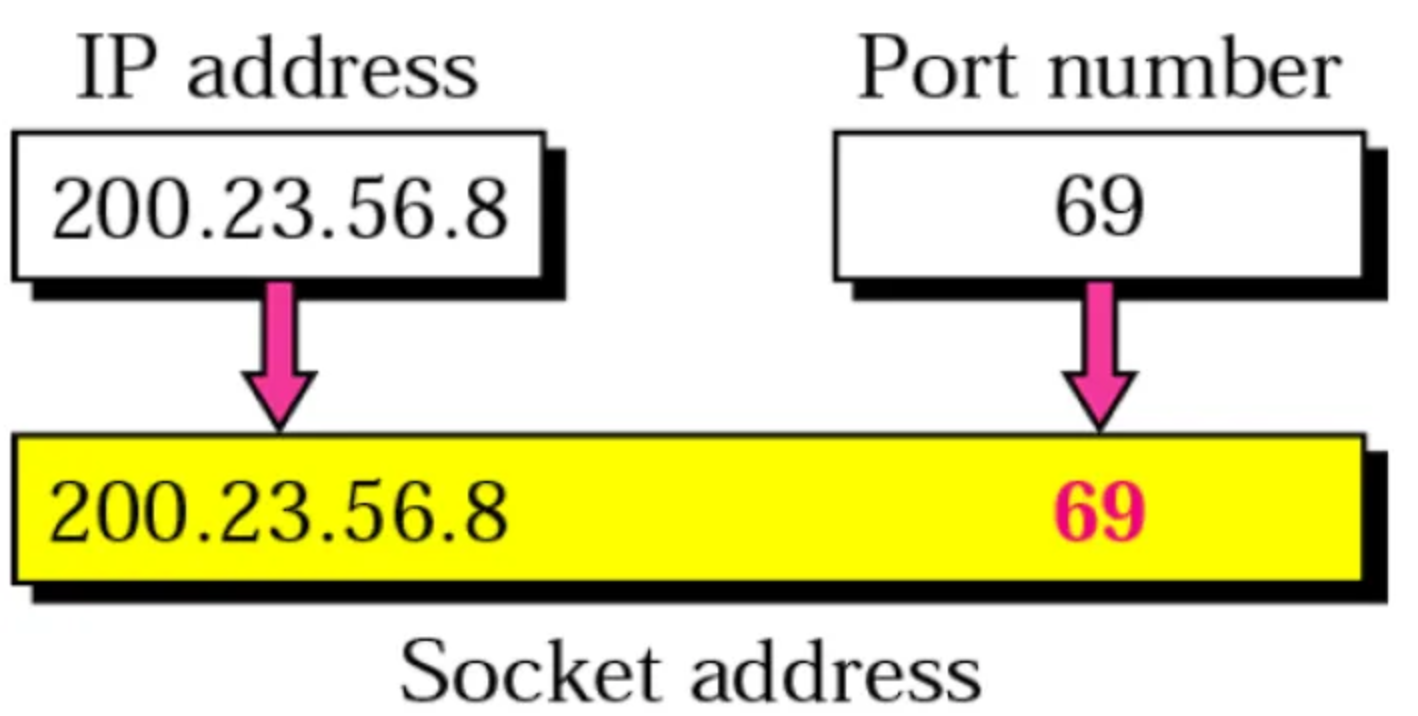
\includegraphics[width=0.6\textwidth]{images/socket_port.png}
    \caption{Relazione tra socket, indirizzo IP e porta}
    \label{fig:socket_port}
\end{figure}

Le porte sono numerate da 0 a 65535 e sono suddivise in tre categorie:
\begin{itemize}
    \item Well-known ports: da 0 a 1023, utilizzate da applicazioni di sistema e protocolli standard (es. HTTP su porta 80, HTTPS su porta 443, DNS(traduce il nome "simbolico" del servizio web per il web server) su porta 53)
    \item Registered ports: da 1024 a 49151, utilizzate da applicazioni registrate presso l'IANA
    \item Dynamic/Private ports: da 49152 a 65535, utilizzate per connessioni temporanee e dinamiche
\end{itemize}

Tramite i numeri di porta è possibile identificare a livello 4 con quale applicazione sto inviando/ricevendo dati

Come identificare un flusso dati in internet?

\begin{figure}[h!]
    \centering
    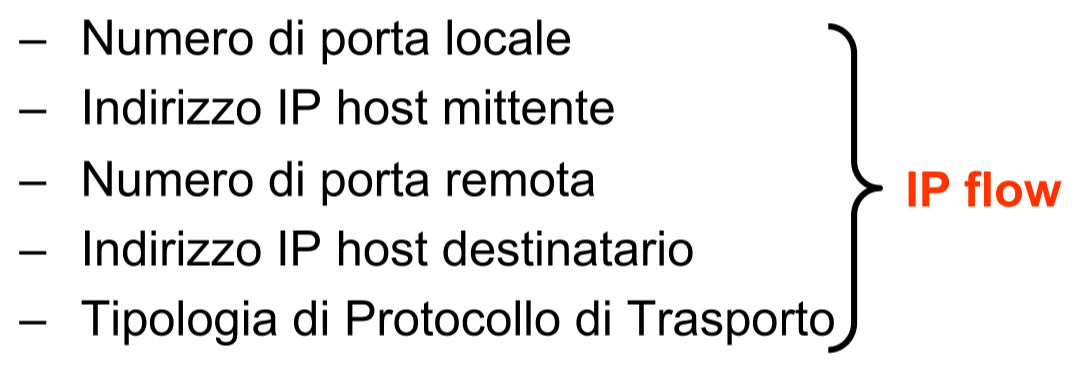
\includegraphics[width=0.5\textwidth]{images/flusso_IP.png}
    \caption{Identificazione di un flusso dati tramite indirizzi IP e numeri di porta (tuple a 4 campi)}
    \label{fig:flussoIP}
\end{figure}

\begin{figure}[h!]
    \centering
    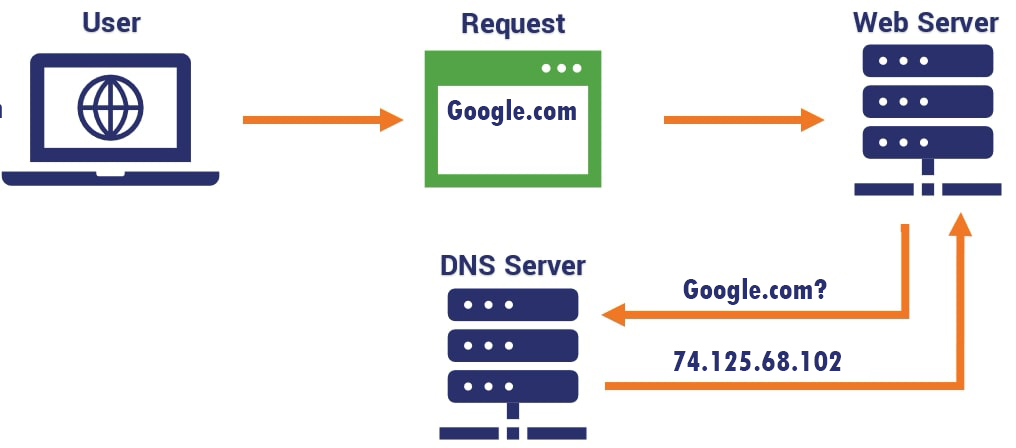
\includegraphics[width=0.5\textwidth]{images/DNS.jpg}
    \caption{Esempio di funzionamento del DNS: risoluzione di un nome simbolico in indirizzo IP, tramite DNS server}
    \label{fig:dns_example}
\end{figure}
traduce nomi comprensibili come www.amazon.com in indirizzi IP utilizzati dai computer, ad esempio 192.0.2.44
\newpage
\section{UDP - datagram}

è il più veloce del TCP poichè non esegue molte funzioni come l'ordinamento dei pacchetti 
i pacchetti sono da 32 bit, ossia 4 byte:
\begin{itemize}
    \item datagram: 16 bit
    \item pseudoheader: 16 bit
\end{itemize}

Si occupa di fare multiplexing(trasmissione) e demultiplexing(ricezione) dei dati, ovvero incapsula i dati dell'applicazione in un pacchetto UDP e aggiunge le informazioni necessarie per la consegna.
Viene usato soprattutto per applicazioni in tempo reale, come servizi streaming live.

\paragraph{Struttura del datagram UDP}

\begin{figure}[h!]
    \centering
    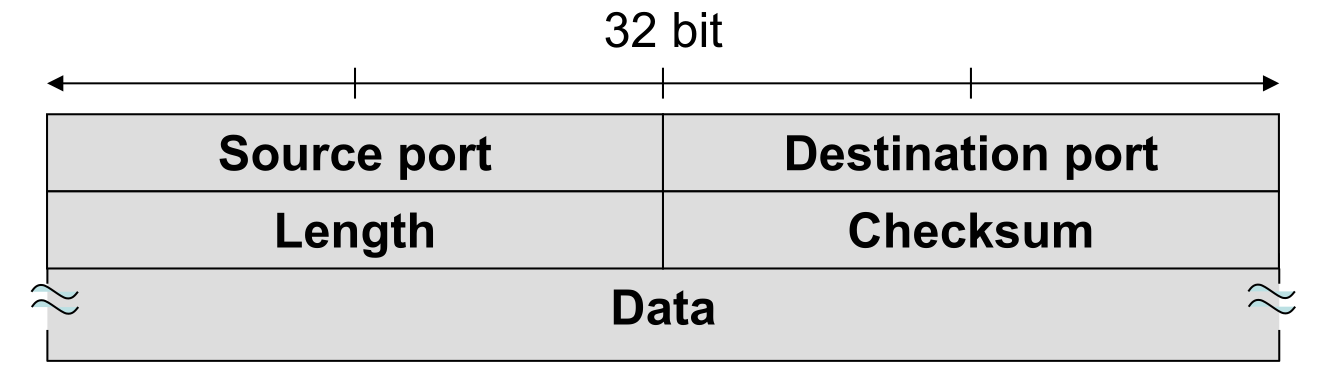
\includegraphics[width=0.7\textwidth]{images/datagram_udp.png}
    \caption{Struttura del datagram UDP}
    \label{fig:datagramudp}
\end{figure}

\begin{itemize}
    \item Source port e destination port(indirizzo IP del mittente/destinatario): 16 bit ciascuno
    \item Length (dimensione del datagram): 16 bit, quindi può rappresentare valori da 0 a $2^{16}-1 = 65535$ bytes, ma il campo include anche l'header, quindi la dimensione massima di un datagram UDP è 65535 byte.
    \item Checksum: 16 bit, utilizzato per verificare l'integrità dei dati del datagram. Il checksum è calcolato su un pseudoheader che include informazioni sull'indirizzo IP del mittente e del destinatario, oltre alla lunghezza del datagram e al protocollo utilizzato (UDP in questo caso). Il pseudoheader non viene trasmesso, ma viene utilizzato solo per il calcolo del checksum. 
    \item Data: dimensione variabile, contiene i dati dell'applicazione
\end{itemize}


\begin{figure}[h!]
    \centering
    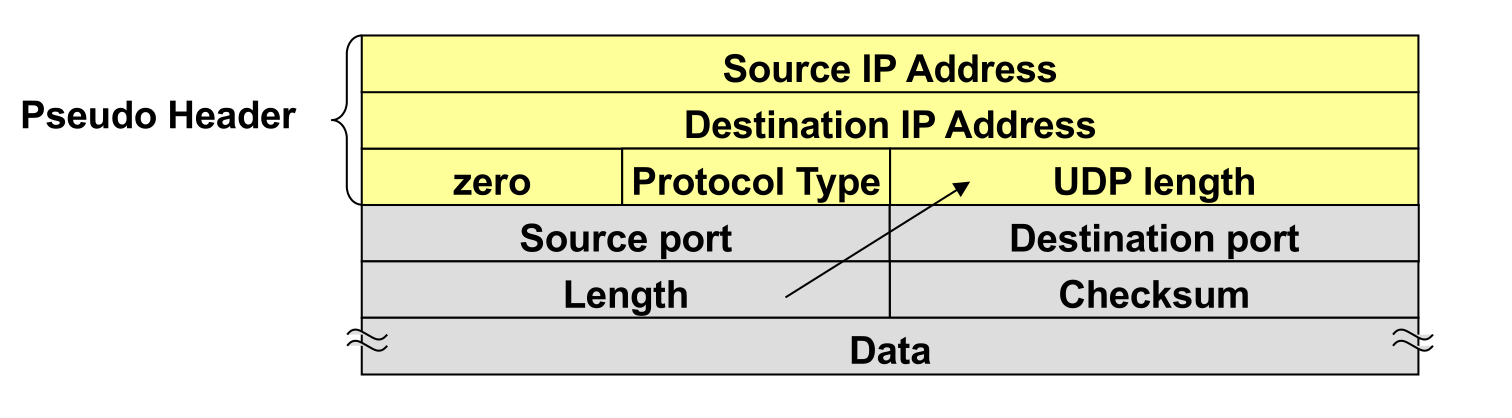
\includegraphics[width=0.7\textwidth]{images/pseudoheaderUDP.png}
    \caption{Pseudoheader UDP utilizzato per il calcolo del checksum}
    \label{fig:psudoheaderudp}
\end{figure}

Nello pseudoheader sono presenti informazioni come il campo Protocol Type viene preso direttamente dal livello 3(protocollo IP).

Il checksum è la somma di controllo, è una tecnica di verifica veloce di controllo errore, non è affidabile al 100\%, è comunque ottimo perchè è veloce  
\begin{itemize}
    \item Se il checksum calcolato è 0xFF(111111111), significa che non ci sono errori, non affidabile.
    \item Se il checksum è diverso da 0xFF, significa che ci sono errori, sicuramente(condizione necessaria).
\end{itemize}
\subsection{Calcolo checksum}
Il valore del checksum prima della trasmissione è impostato a 0.
 \paragraph{In trasmissione}
In tramissione vengono sommate in binario tutte le righe(mezze righe da 16 bit) del datagram, faccio il complemento ad 1(NOT) di questo risultato. Questo è il checksum inviato nel datagram di trasmissione.
\paragraph{In ricezione}
In ricezione viene ricevuto il datagram, con all'interno il checksum calcolato precedentemente in trasmissione. 

Viene calcolato nuovamente il checksum del datagram ricevuto, sommando in binario tutte le righe(mezze righe da 16 bit) del datagram, e sommandolo al checksum ricevuto. 

Se il risultato è diverso da 1 significa che i due valori calcolati in ricezione e trasmissione sono differenti, perciò c'è un errore.


\begin{figure}[h!]
    \centering
    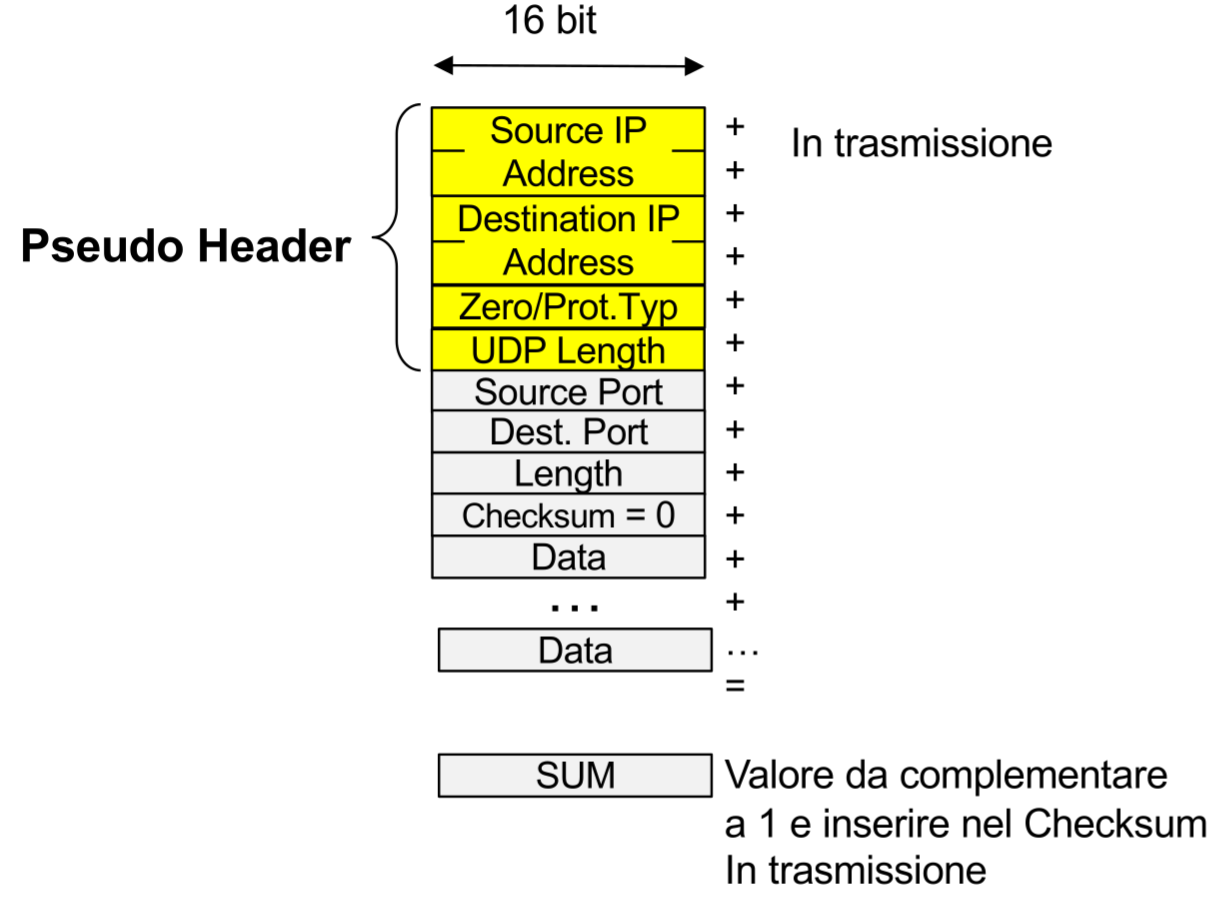
\includegraphics[width=1\textwidth]{images/checksum_udp.png}
    \caption{Esempio di calcolo del checksum UDP}
    \label{fig:checksumudp}
\end{figure}

\newpage
\section{TCP - segmento}
Nei processi TCP viene utilizzata una coppia di socket per identificare un flusso di dati. Ogni socket è identificato da una tupla a 4 campi:
\begin{multicols}{2}
\begin{itemize}
    \item Indirizzo IP del mittente
    \item Porta del mittente
    \item Indirizzo IP del destinatario
    \item Porta del destinatario
\end{itemize}
\end{multicols}

La connessione è full duplex $\rightarrow$ comunicazione affidabile, se qualcosa va storto chiede la ritrasmissione del pacchetto errato.

Il tcp è un protocollo greedy, ingordo, tende a prendere tutta la banda di cui necessita; questo protocollo non evita le congestioni ma le provoca, però quando le provoca cerca di risolverle.

L'affidabilitò di TCP sta nei riscontri cumulativi che gli permettono di gestire le seguenti problematiche:
\begin{itemize}
    \item Controllo di congestione e2e: regolazione del rate di trasmissione così da utilizzare completamente la banda disponibile evitando che la rete collassi
    \item Controllo del flusso e2e: regolarizza il rate di trasmissione per evitare la saturazione del buffer di ricezione
\end{itemize}

\begin{figure}[h!]
    \centering
    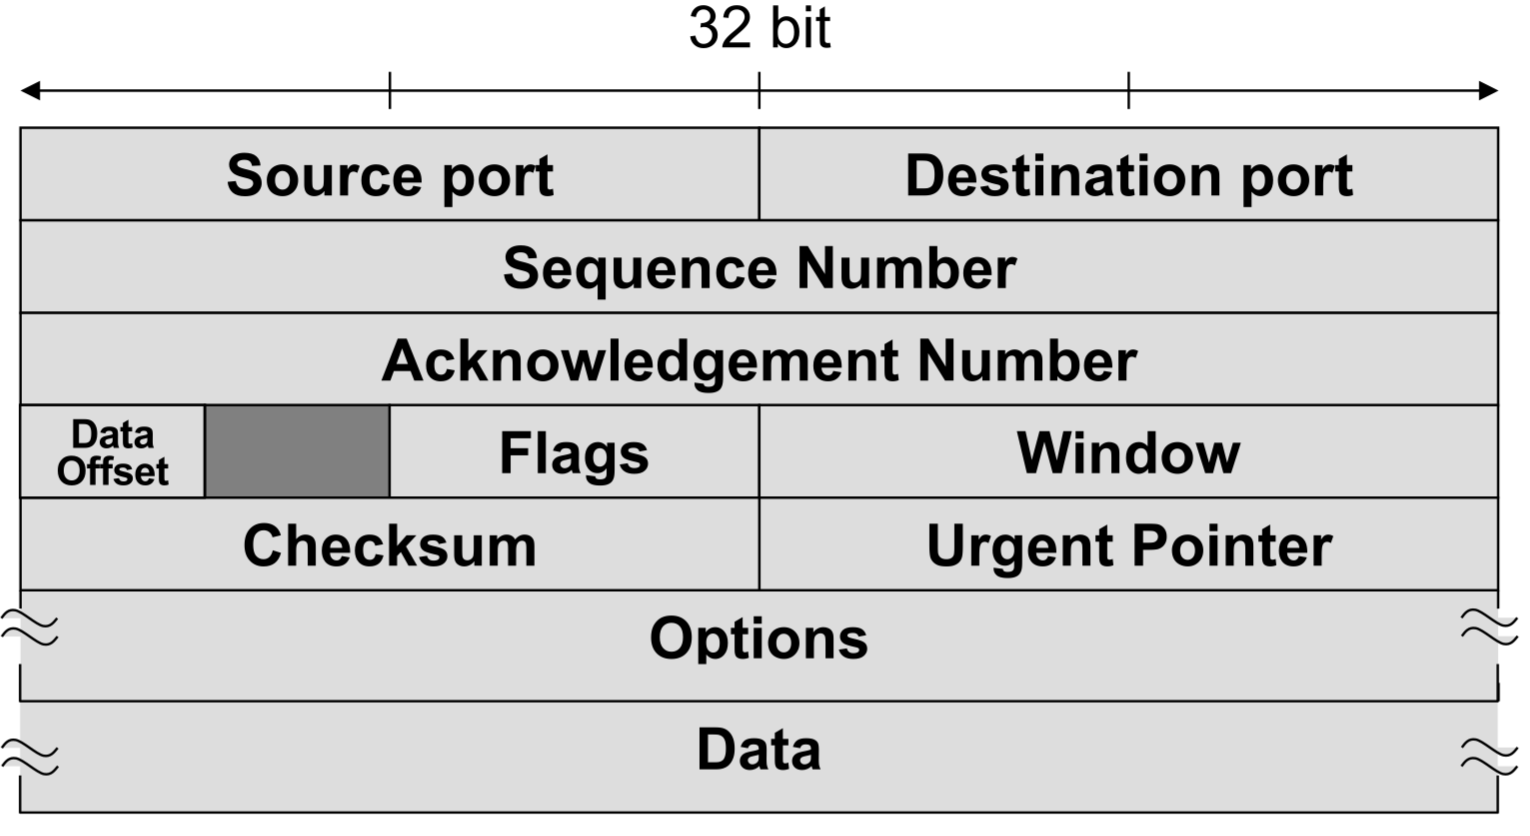
\includegraphics[width=0.8\textwidth]{images/segmento_tcp.png}
    \caption{Struttura del segmento TCP}
    \label{fig:segmentotcp}
\end{figure}

I pacchetti in tcp vengono chiamati segmenti, così strutturati:
\begin{itemize}
    \item source port/destination port: 16 bit ciascuna e identificano il mittente e il destinatario del segmento
    \item sequence number: 32 bit, numero di sequenza del primo byte del segmento, utilizzato per ordinare i segmenti ricevuti ; i byte del livello applicativo (che costituiranno il payload dei
diversi segmenti trasmessi) sono numerati in modo continuo partendo da un valore casuale(zero relativo). 

Nel campo Seq. Number si inserisce poi il numero di sequenza (di questa numerazione continua)
relativo al primo byte contenuto nel campo Data
\begin{figure}[h!]
    \centering
    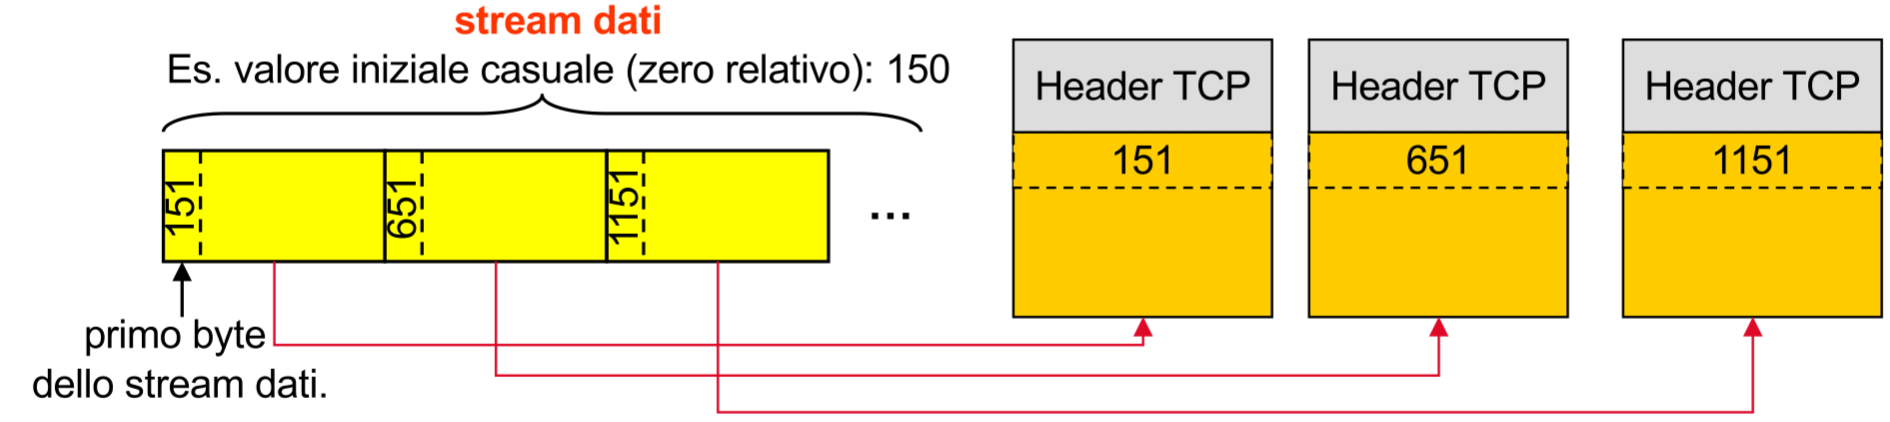
\includegraphics[width=0.9\textwidth]{images/sequence_number.png}
    \caption{Esempio di utilizzo del campo Sequence Number nei segmenti TCP}
    \label{fig:sequencenumber}
\end{figure}
    \item ackwoledgment number: 32 bit, nel campo ack.number si inserisce il numero di sequenza del primo byte che ci si aspetta di ricevere (quindi il numero di sequenza del primo byte che non è stato ricevuto), si usa per capire fino a che punto il segmento è stato ricevuto correttamente. Così facendo so anche da che punto riprendere la trasmissione dei dati.(è utile a dare un riscontro di ciò che mi sta inviando il mittente, tenendolo aggiornato sulla correttezza di ciò che mi ha inviato, connessione full duplex appunto); può essere anche un campo vuoto, 0.
    \item data offset: 4 bit, indica la lunghezza dell'header del TCP
    \item flags: 6 bit, sono dei flag di controllo che indicano lo stato della connessione TCP:
    \begin{itemize}
        \item URG: indica se il segmento contiene dati urgenti.
        \item ACK: acknowledgment number
        \item PSH: push, richiesta di invio immediato dei dati al livello applicativo
        \item RST, SYN, FIN: reset, synchronize, finish della connessione 
        \end{itemize}
    \item window: è un campo utilizzato nella gestione del controllo di flusso, indica la dimensione della finestra di ricezione, ovvero la quantità di dati che il mittente può inviare prima di ricevere un acknowledgment dal destinatario. La dimensione della finestra può variare durante la connessione in base alla disponibilità di buffer del destinatario.
    \item urgent pointer: indica i dati che il ricevitore deve elaborare per prima
    \item checksum: è come in UDP
    \item options: almeno 32 bit, è opzionale, può contenere info di configurazione del segmento TCP 
\end{itemize}


\subsection{Apertura connessione client-server (3way handshake)}
 
\begin{figure}[h!]
    \centering
    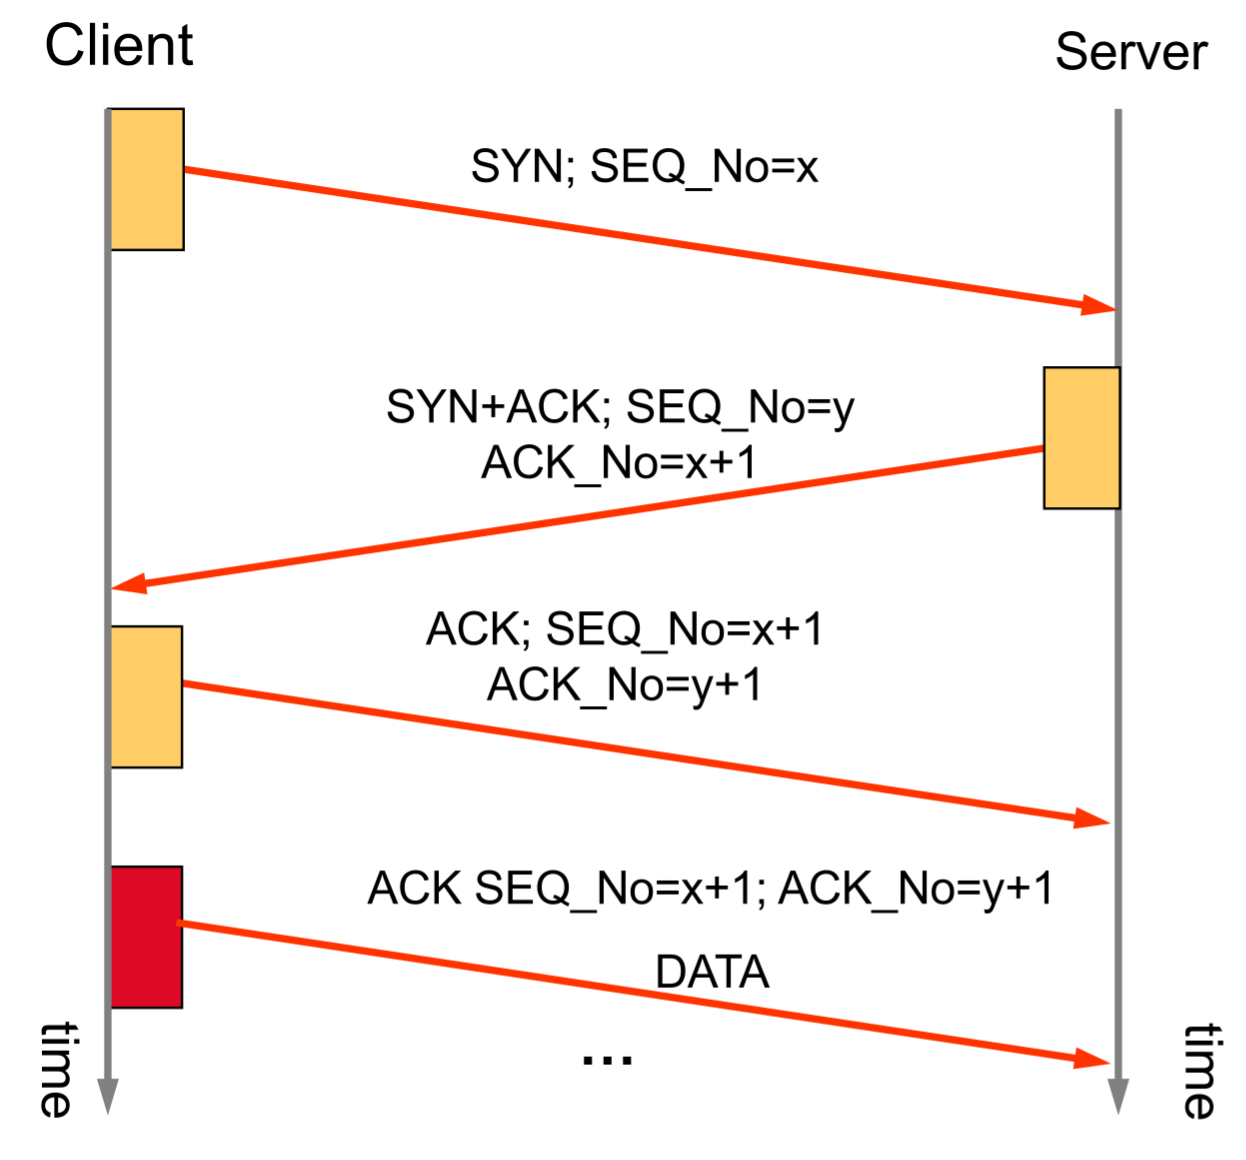
\includegraphics[width=0.7\textwidth]{images/three_w_hs1.png}
    \caption{Three-way handshake: stabilimento della connessione TCP tra client e server}
    \label{fig:threewayhandshake}
\end{figure}

La connessione viene sempre aperta dal client.

Quando ricevo un segmento ho bisogno di sapere in che modo sta contando i byte il mittente; 

Il client sceglie lo zero relativo, ossia il numero di sequenza(sequence number scelto casualmente, $SEQ.NUMBER = x$) da cui partire per numerare i byte che invierà al server, inviando un segmento vuoto in cui setta il flag $SYN = 1$,($ACK = 0$ all'inizio della comunicazione) così da iniziare la comunicazione.

A questo punto il server risponde alla richiesta del client, inviando:
\begin{itemize}
    \item un segmento vuoto con $SYN = 1$ e $ACK = 1$(questo flag a 1 fa capire al client che il campo ACKNUMBER è stato modificato), in cui il numero di sequenza è $SEQ.NUMBER = y$(per i dati che il server invierà, non dimenticare che la comunicazione è full duplex) e il numero di ack è $ACK.NUMBER = x + 1$ (il server ha ricevuto la richiesta del client, quindi il numero di ack è incrementato di 1)
    \item un segmento con i dati richiesti dal client, in cui il numero di sequenza è $SEQ.NUMBER = y + 1$ e il numero di ack è $ACK.NUMBER = x + 1$
\end{itemize}

 

Per terminare la "conversazione" il client invia un segmento(vuoto, ossia senza dati) con il flag SYN a 0, e conferma la corretta ricezione del messaggio precedente (y) con l'ACK.NUMBER ricevuto dal server più di 1(y + 1).

Quello in rosso nell'immagine è un ulteriore segmento, uguale al precedente, ma "pieno", ossia con i dati da inviare.

\subsection{Chiusura connessione}
La chiusura della connessione puà essere avviata da uno dei due host, il client o il server(tipicamente la chiude il client).

\begin{figure}[h!]
    \centering
    \begin{minipage}{0.48\textwidth}
        \centering
        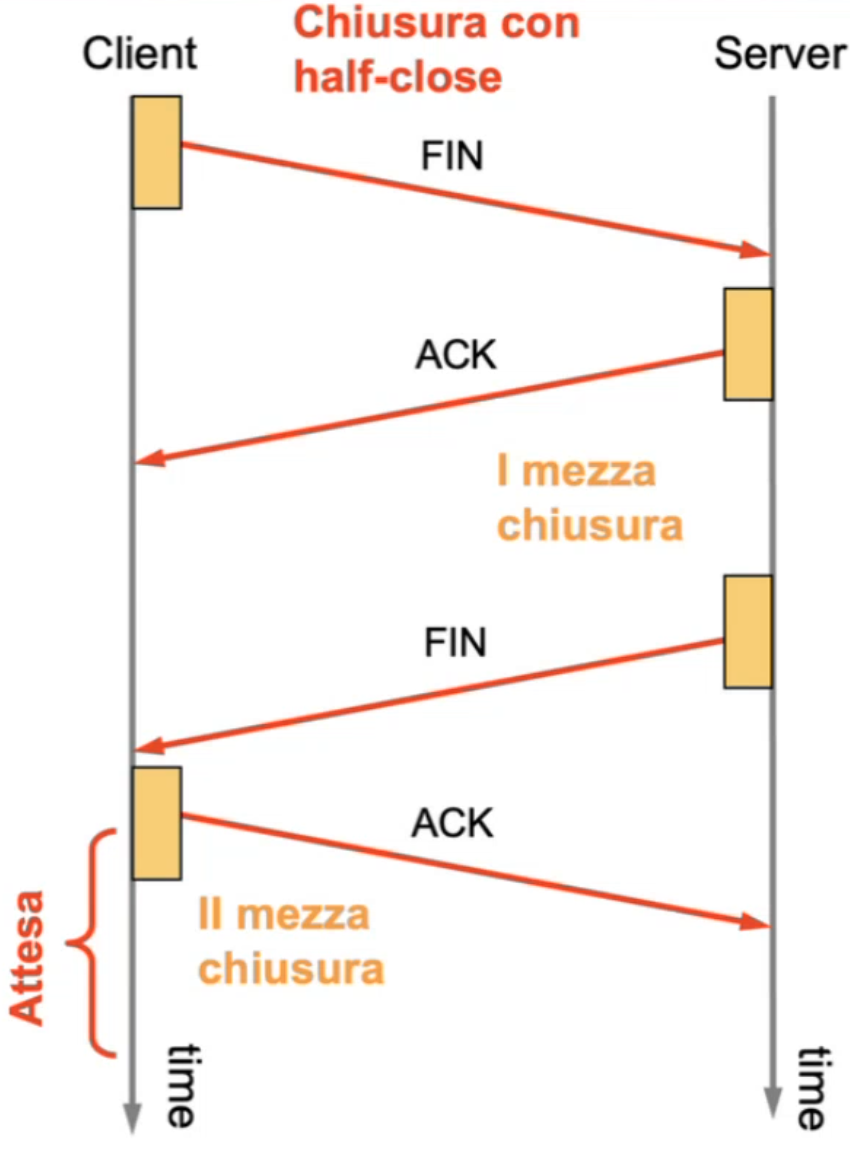
\includegraphics[width=\textwidth]{images/halfclosetcp.png}
        \caption{Chiusura della connessione TCP tramite half-close}
        \label{fig:halfclosetcp}
    \end{minipage}\hfill
    \begin{minipage}{0.48\textwidth}
        \centering
        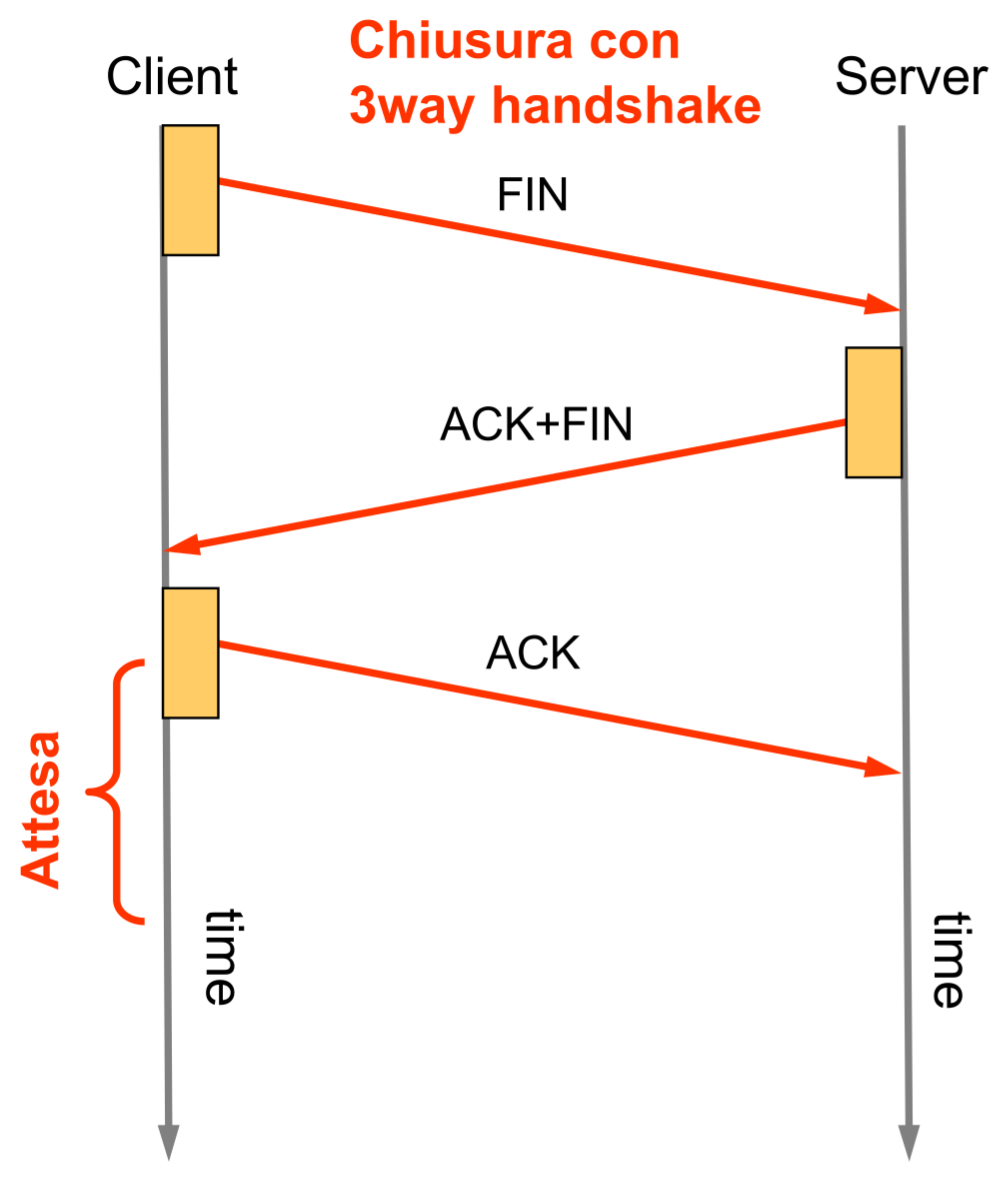
\includegraphics[width=\textwidth]{images/3wayclose.png}
        \caption{Chiusura della connessione TCP tramite 3-way handshake}
        \label{fig:3wayclose}
    \end{minipage}
\end{figure}

\paragraph{Chiusura con half-close}
La chiusura della connessione avviene tramite due mezze chiusure:
\begin{itemize}
    \item prima mezza chiusura:
    \begin{itemize}
            \item Il client invia un segmento VUOTO con il flag FIN a 1, per indicare che non invierà più dati al server.(inizio I mezza chiusura) 
            \item Il server  ivnia un segmento VUOTO con il flag ACK per confermare la prima mezza chiusura; allora il server continua ad inviare i dati finchè non termina, pronto per inziare con la seconda mezza chiusura(fine I mezza chiusura)
    \end{itemize}
    \item seconda mezza chiusura:
    \begin{itemize}
            \item Il server invia un segmento con il flag FIN a 1 e il flag ACK a 1, per indicare che non invierà più dati al client.(inizio II mezza chiusura) 
            \item Il client risponde con un segmento con il flag ACK a 1, per confermare la ricezione della richiesta di chiusura del server. (fine II mezza chiusura)
    \end{itemize}
\end{itemize} 


\newpage
\paragraph{Chiusura con 3way handshake}

in risposta al segmento FIN inviato
dal client, il server invia un unico segmento con
FIN+ACK settati (e con eventualmente gli ultimi
dati).

Questa soluzione non prevede che il server invii
ulteriori dati e il client risponde con il segmento di ACK di
chiusura della connessione.



\paragraph{TIMEWAIT}
in entrambe le tecniche (con
half-close o 3way handshake) dopo il segmento
di ACK si avvia un timer (Time Wait) prima della
definitiva chiusura della connessione. Può
succedere, infatti, che il segmento ACK vada
perso e il server ritrasmetta il suo FIN. Il client
deve quindi essere ancora in grado di poter
ritrasmettere l'ACK finale.

\paragraph{Piggybacking} è la trasmissione di riscontri in
pacchetti che trasportano anche dati, quindi non c'è bisogno di riscontrare utilizzando pacchetti vuoti ma si può fare anche con pacchetti con dati 
\newpage
\subsection{TCP sequenze di stati}
\subsubsection{TCP client}
\begin{figure}[h!]
    \centering
    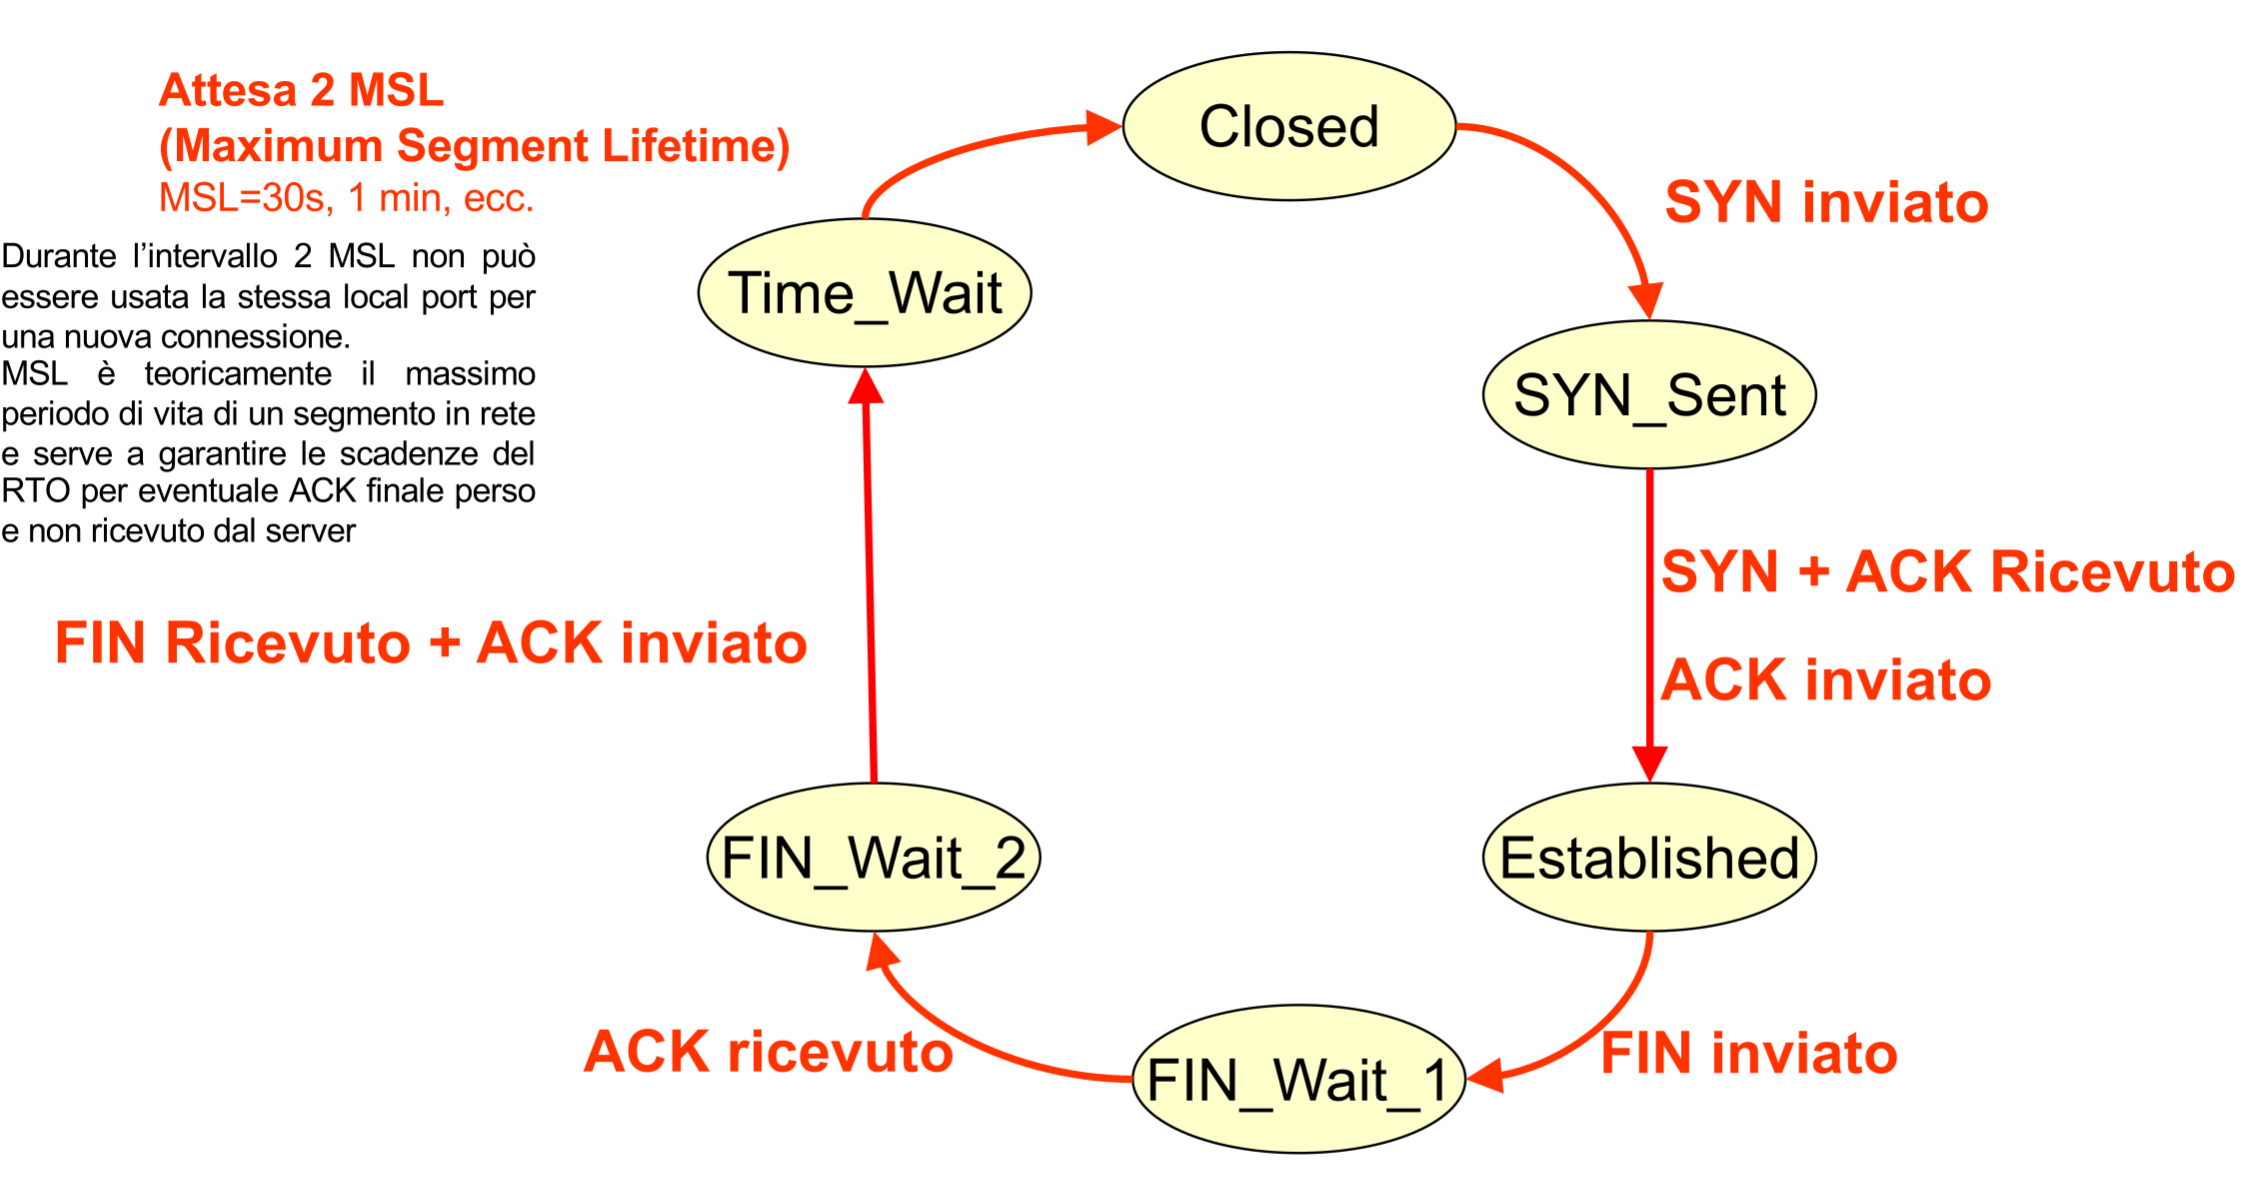
\includegraphics[width=1.1\textwidth]{images/tcpstaticlient.png}
    \caption{Sequenza di stati TCP lato client}
    \label{fig:tcpstaticlient}
\end{figure}
\subsubsection{TCP server}

\begin{figure}[h!]
    \centering
    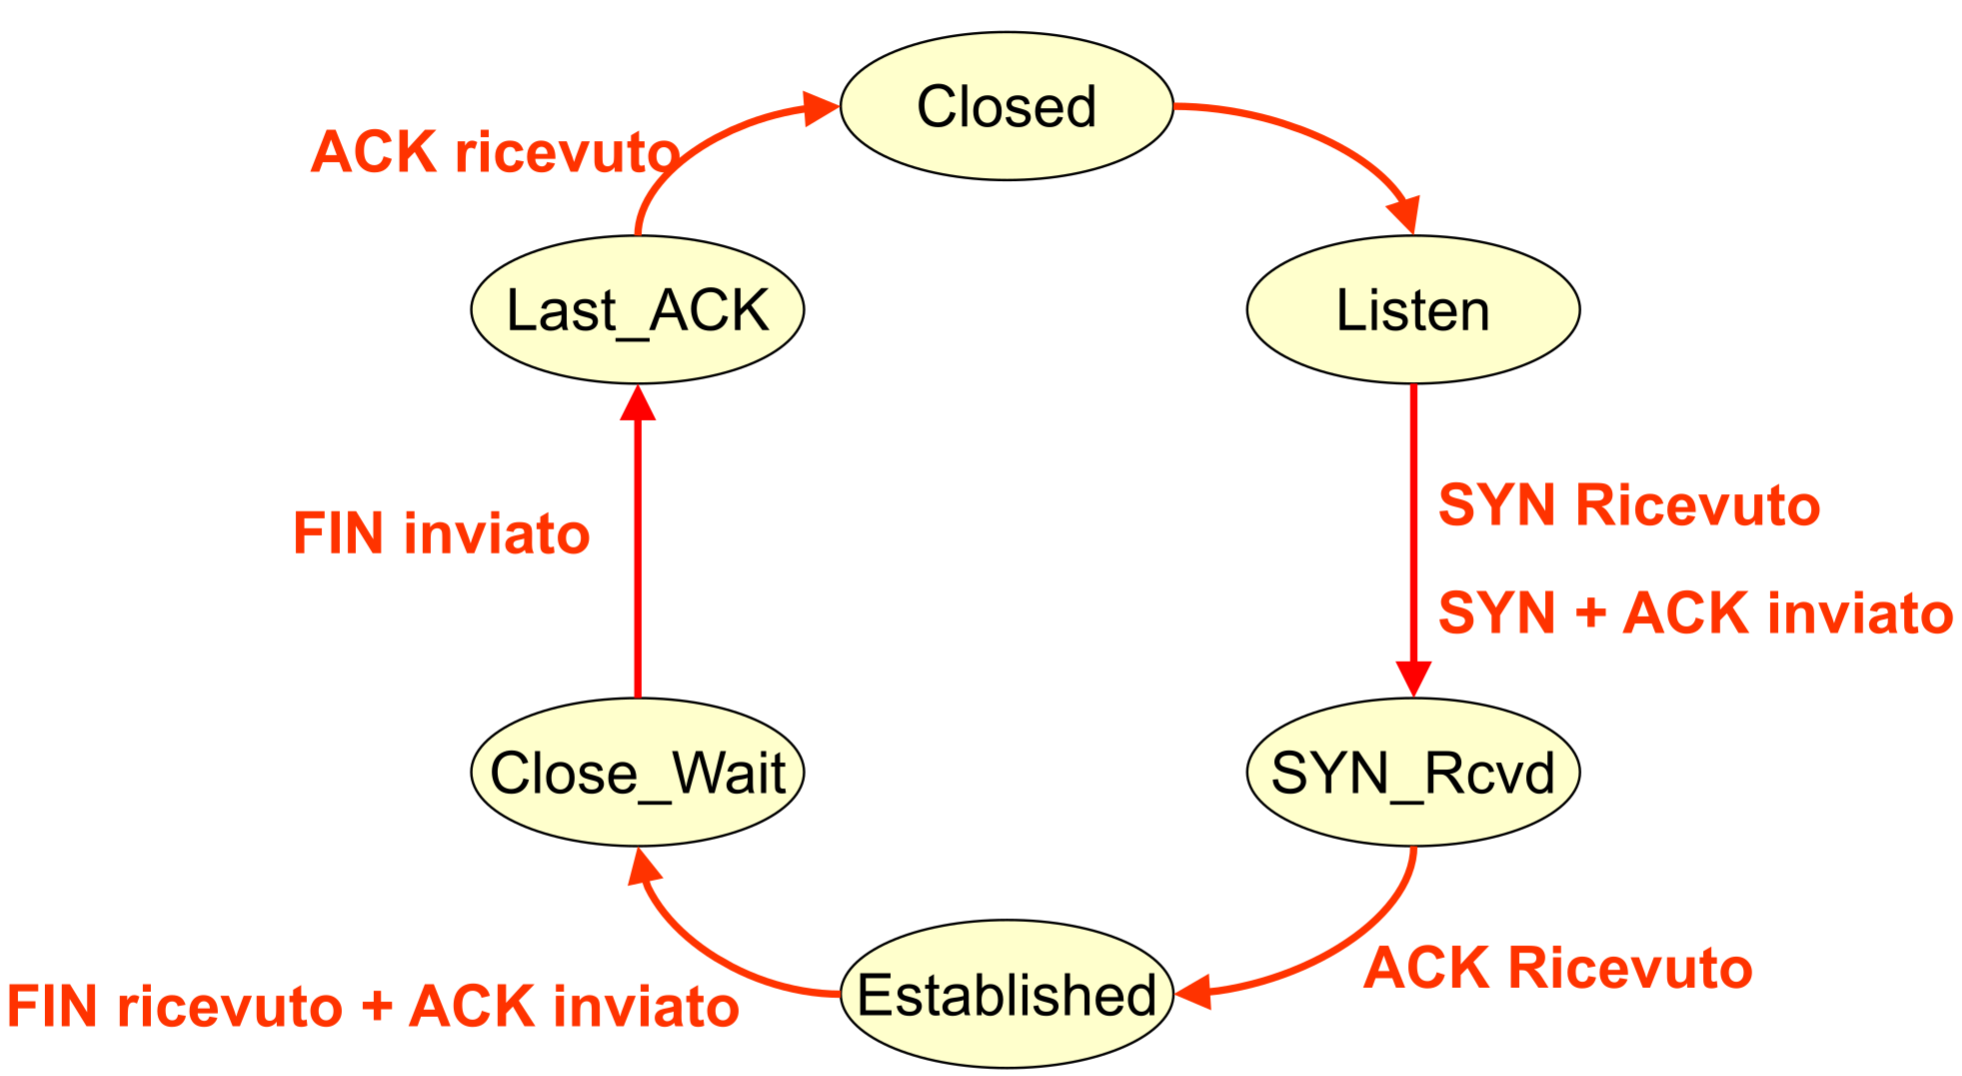
\includegraphics[width=1\textwidth]{images/tcpstatiserver.png}
    \caption{Sequenza di stati TCP lato server}
    \label{fig:tcpstateserver}
    \end{figure}
\newpage

\subsection{Trasmissione dei segmenti - sliding window}
Il TCP usa un meccanismo di trasmissione dei segmenti basato su finestre scorrevoli, finestra di trasmissione e finestra di ricezione; in base alla loro larghezzo si possono inviare più o meno bytes.

Attua "self-clocking", ossia il mittente regola la velocità di invio dei segmenti in base alla velocità di ricezione del destinatario. Non c'è una velocità fissa delle sliding windows.

 \subsubsection{Round trip time - RTT}
Quando invia un segmento, il mittente deve attendere un certo tempo prima di ricevere un (riscontro)acknowledgment dal destinatario. Questo tempo è chiamato round trip time (RTT) e rappresenta il tempo necessario per inviare un segmento e ricevere l'ACK.
 
Data W, dimensione della finestra di trasmissione, e RTT, il tempo di round trip, la velocità media di trasmissione dei segmenti è data da:

\begin{equation}
    \text{rate medio} = \frac{W}{RTT}
\end{equation}

Come miglioro questo rate? 

Si può agire solo sulla dimensione della finestra W, non sul RTT.

\begin{figure}[h!]
    \centering
    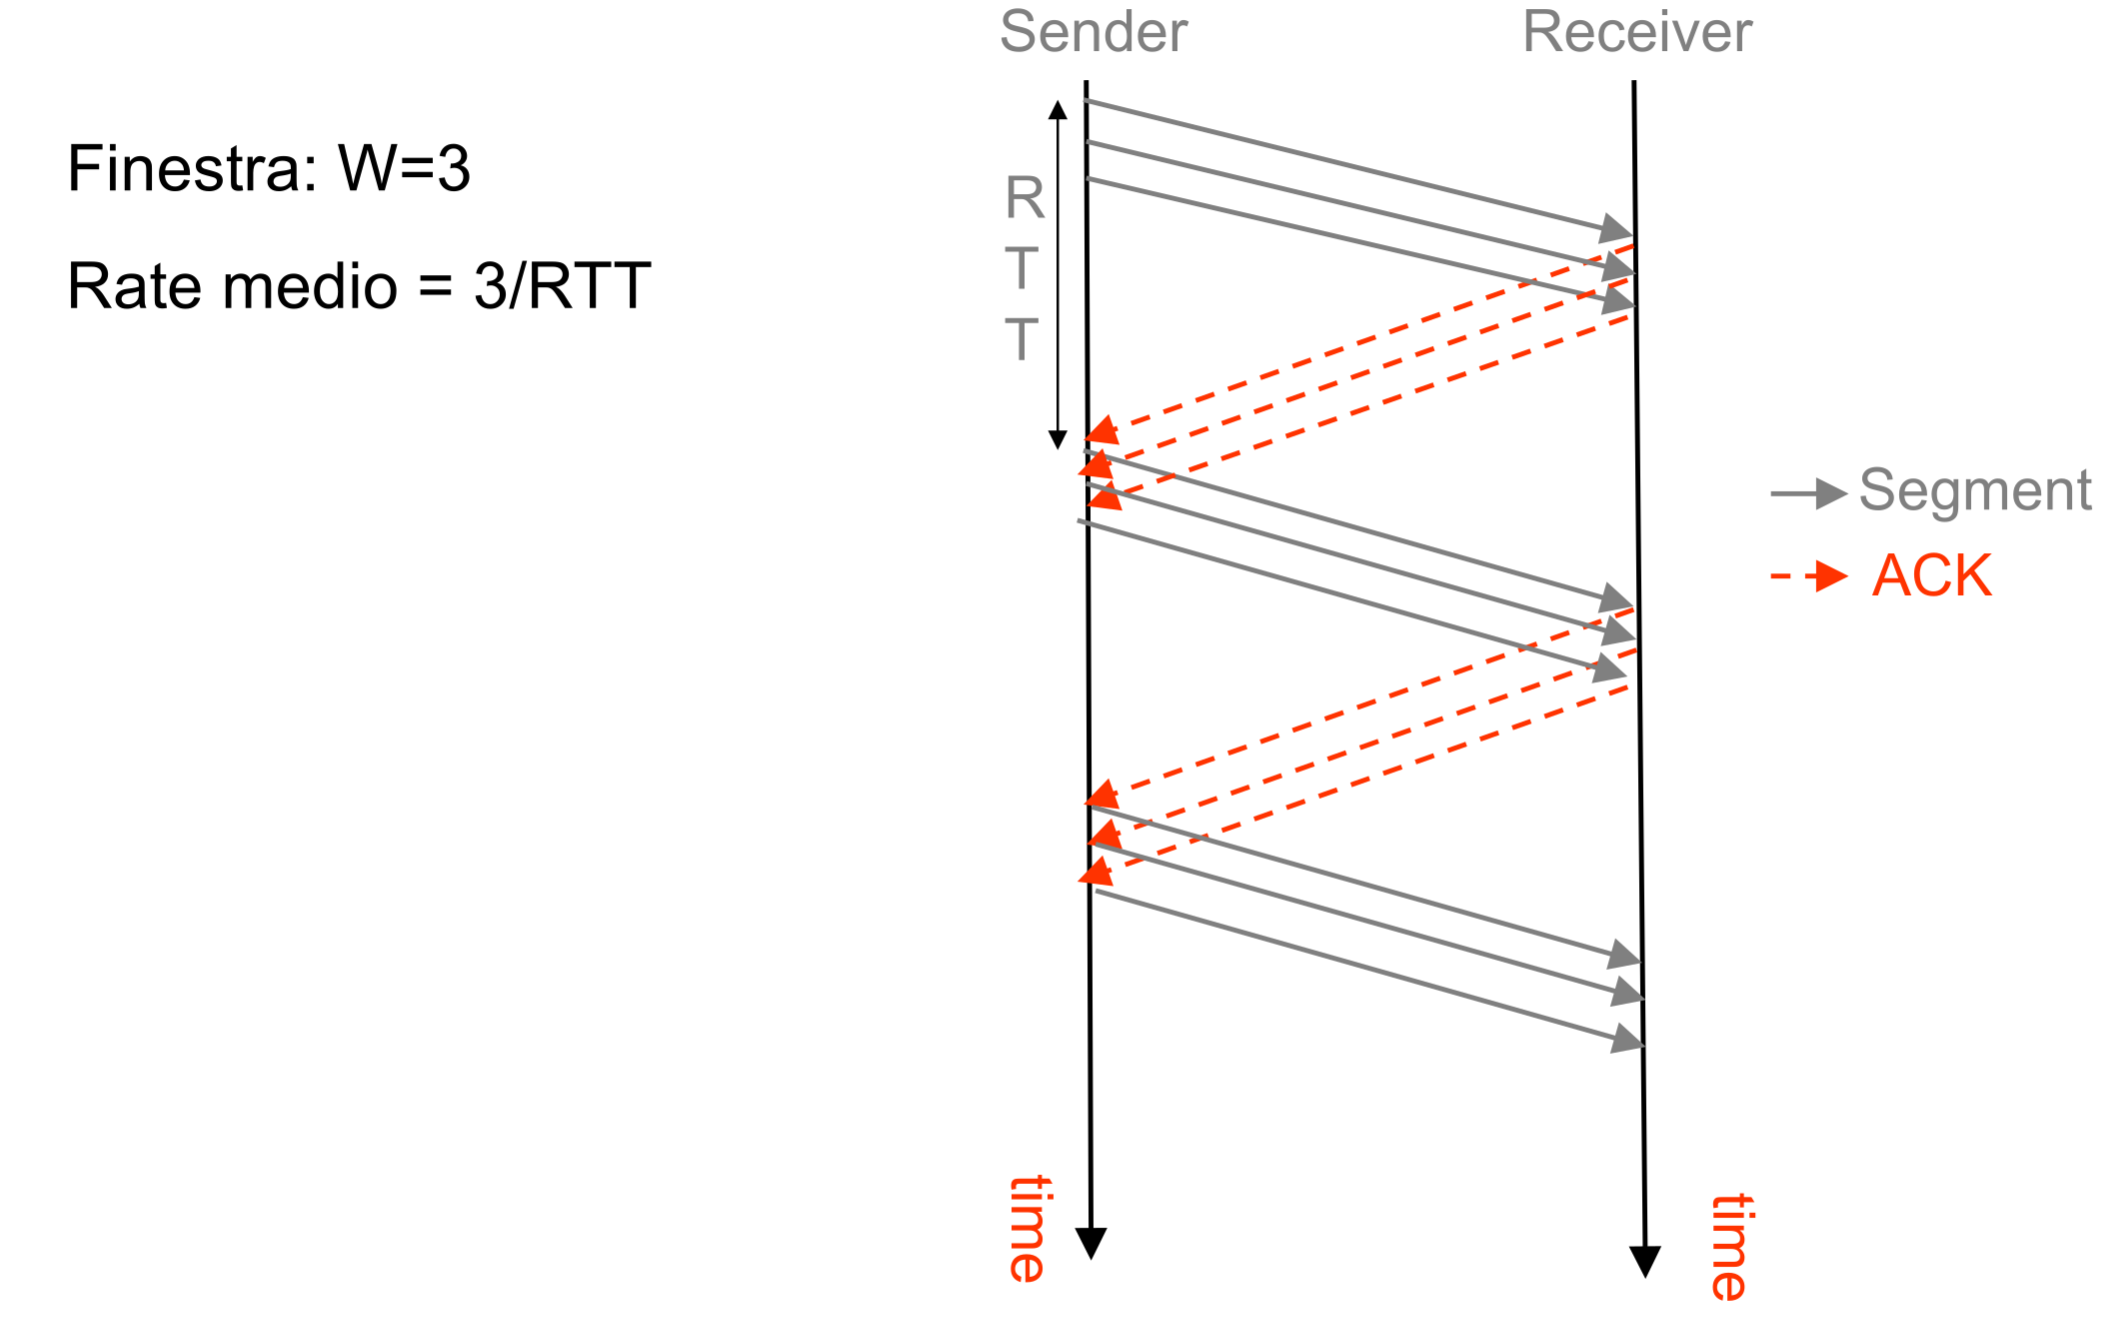
\includegraphics[width=1\textwidth]{images/rttsliding.png}
    \caption{Esempio di sliding window e round trip time (RTT)}
    \label{fig:rttsliding}
\end{figure}
\newpage

\subsection{Finestre di trasmissione e ricezione}
\begin{figure}[h!]
    \centering
    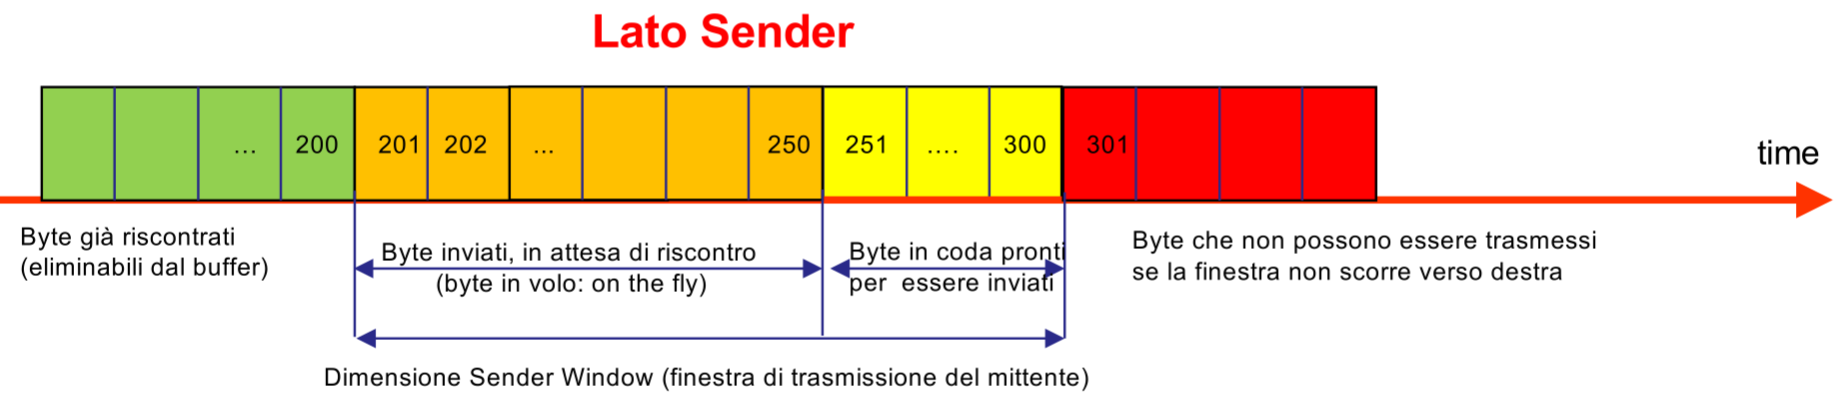
\includegraphics[width=1\textwidth]{images/finestratrasmissione.png}
    \caption{Esempio di finestra di trasmissione}
    \label{fig:finestratrasmissione}
\end{figure}

Sono gli ACK ricevuti che fanno scorrere la finestra. Se ricevo l'ACK 240 allora la finestra scorre fino a 240(riscontri cumulativi, non devo dicevere quelli 201, 202 ecc..., ma mi basta 240 per scorrere anche tutti i byte precedenti a 240).




\begin{figure}[h!]
    \centering
    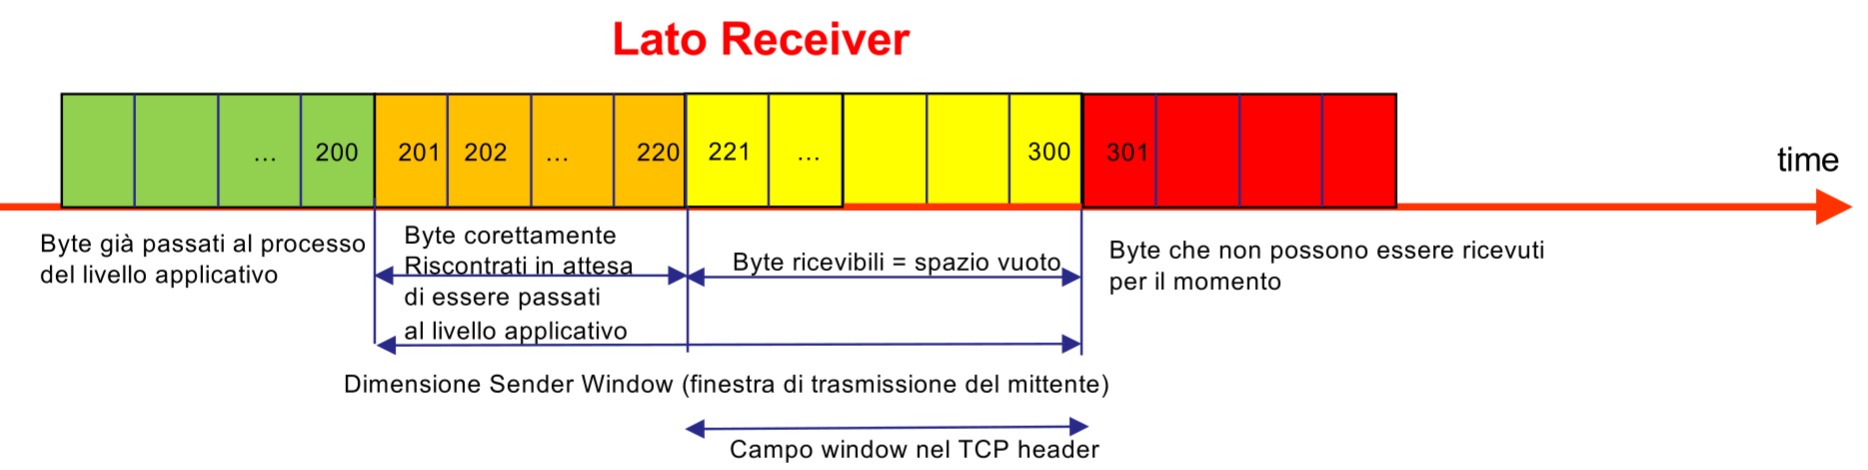
\includegraphics[width=1\textwidth]{images/finestraricezione.png}
    \caption{Esempio di finestra di ricezione}
    \label{fig:finestraricezione}
\end{figure}



\subsection{Controllo di flusso - come gestisce il TCP il flusso dei dati?}

\begin{figure}[h!]
    \centering
    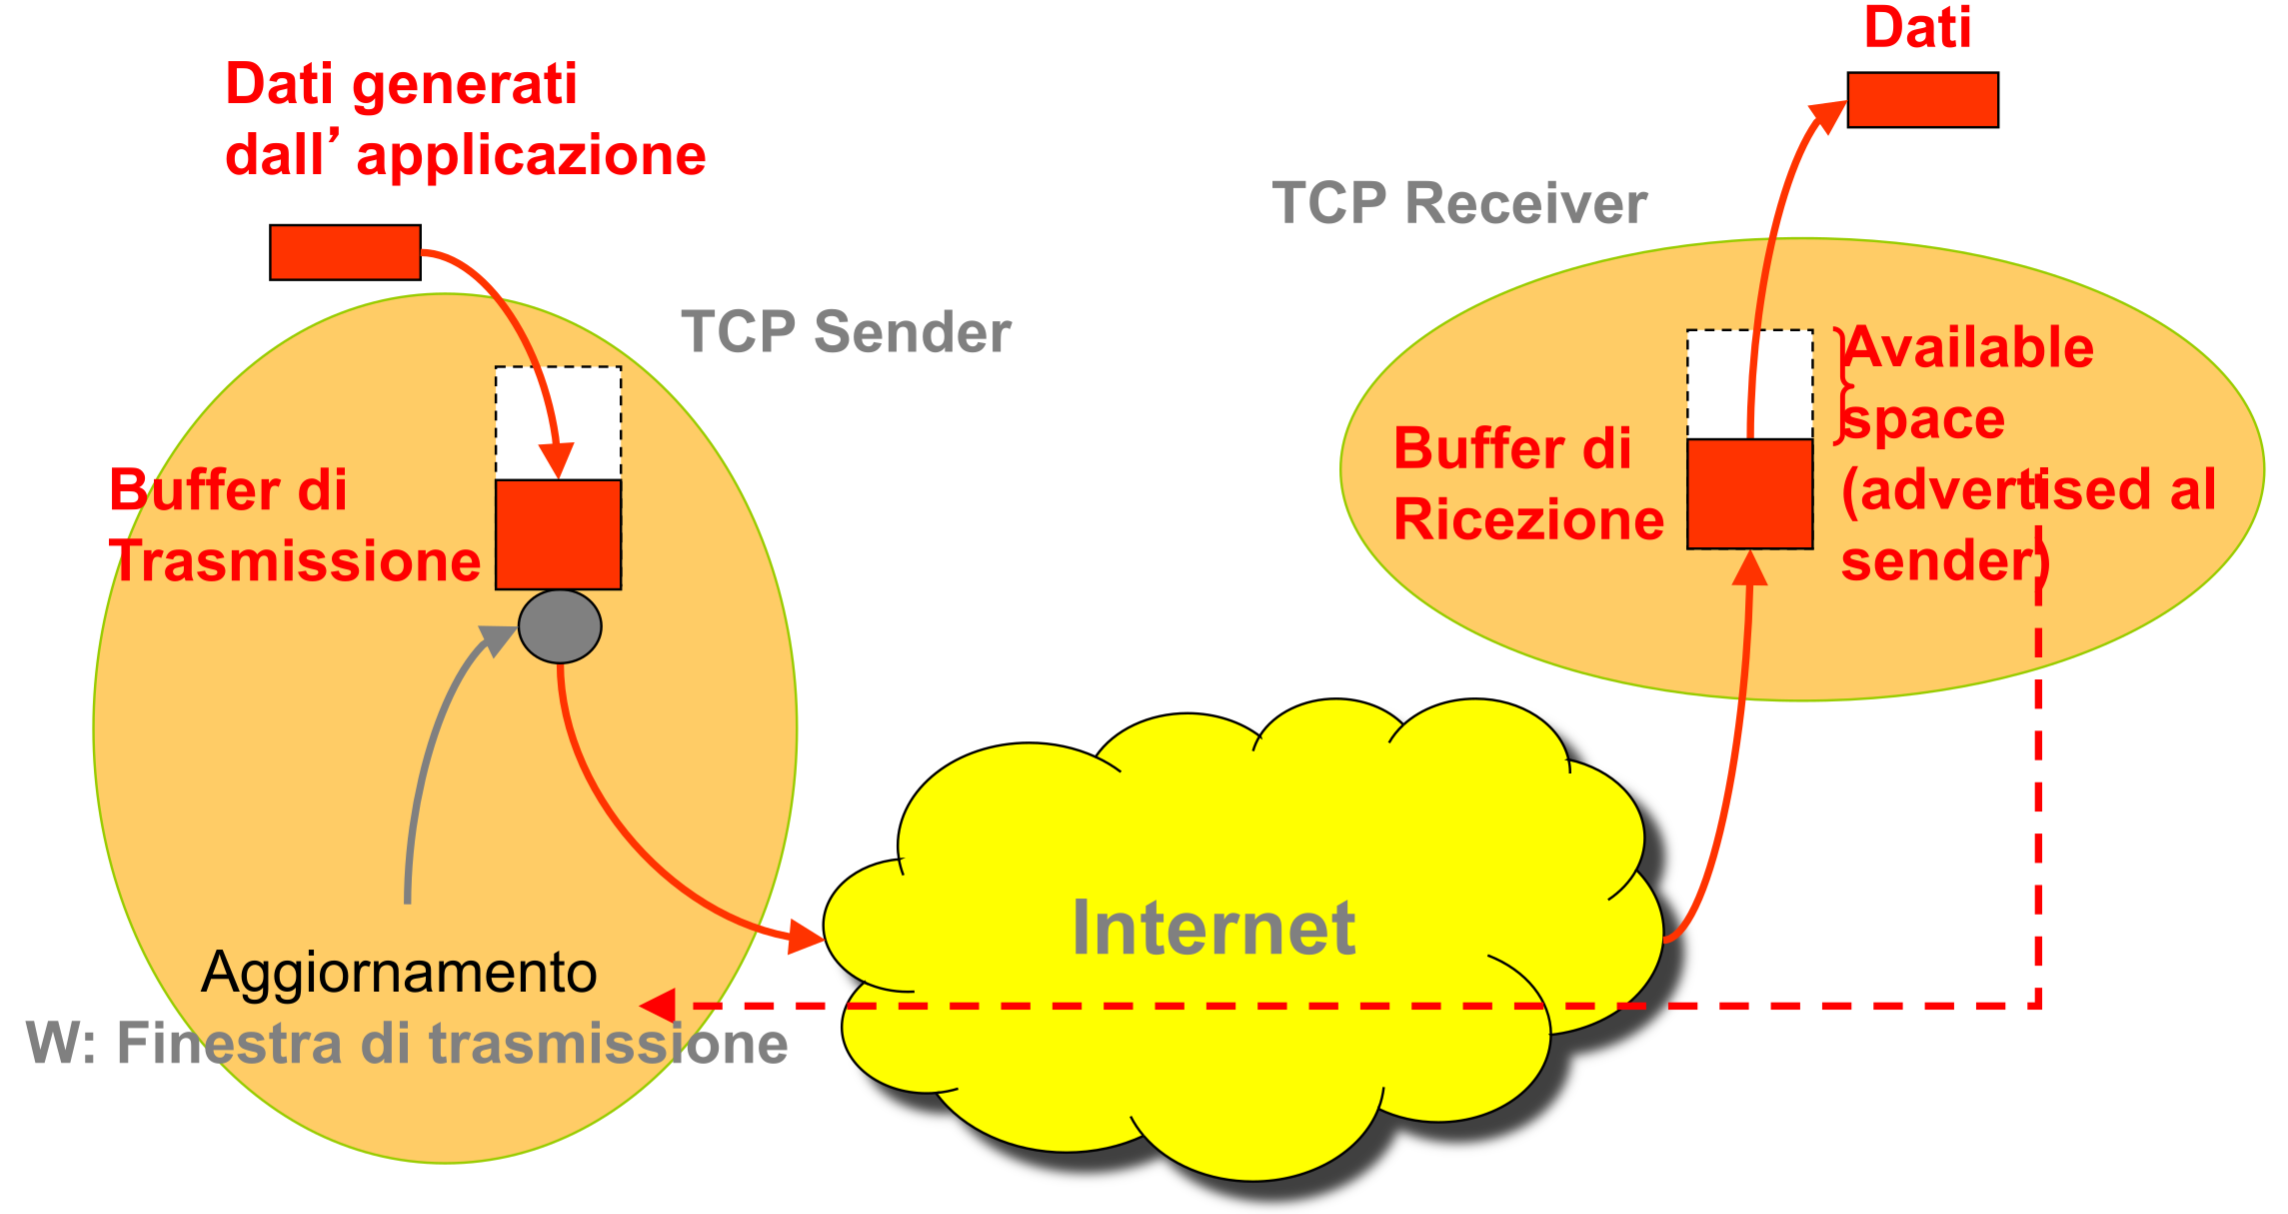
\includegraphics[width=0.8\textwidth]{images/tcpflusso.png}
    \caption{Esempio di flusso TCP}
    \label{fig:tcpflusso}
\end{figure}


IMPORTANTE: ciò che è presente nel buffer di ricezione è stato riscontrato dal mittente.

Il receiver comunica con il sender la dimensione del buffer di ricezione, in modo che il mittente possa regolare la velocità di invio dei segmenti, quindi regolare la finestra di trasmissione.


\newpage
\subsection{Perdita di segmenti - RTO e 3 dupack} 
Si assume che un segmento sia stato perso se si verificano: 3 dupack, RTO.

 \subsubsection{Retransmission Time Out - RTO}
\begin{figure}[h!]
    \centering
    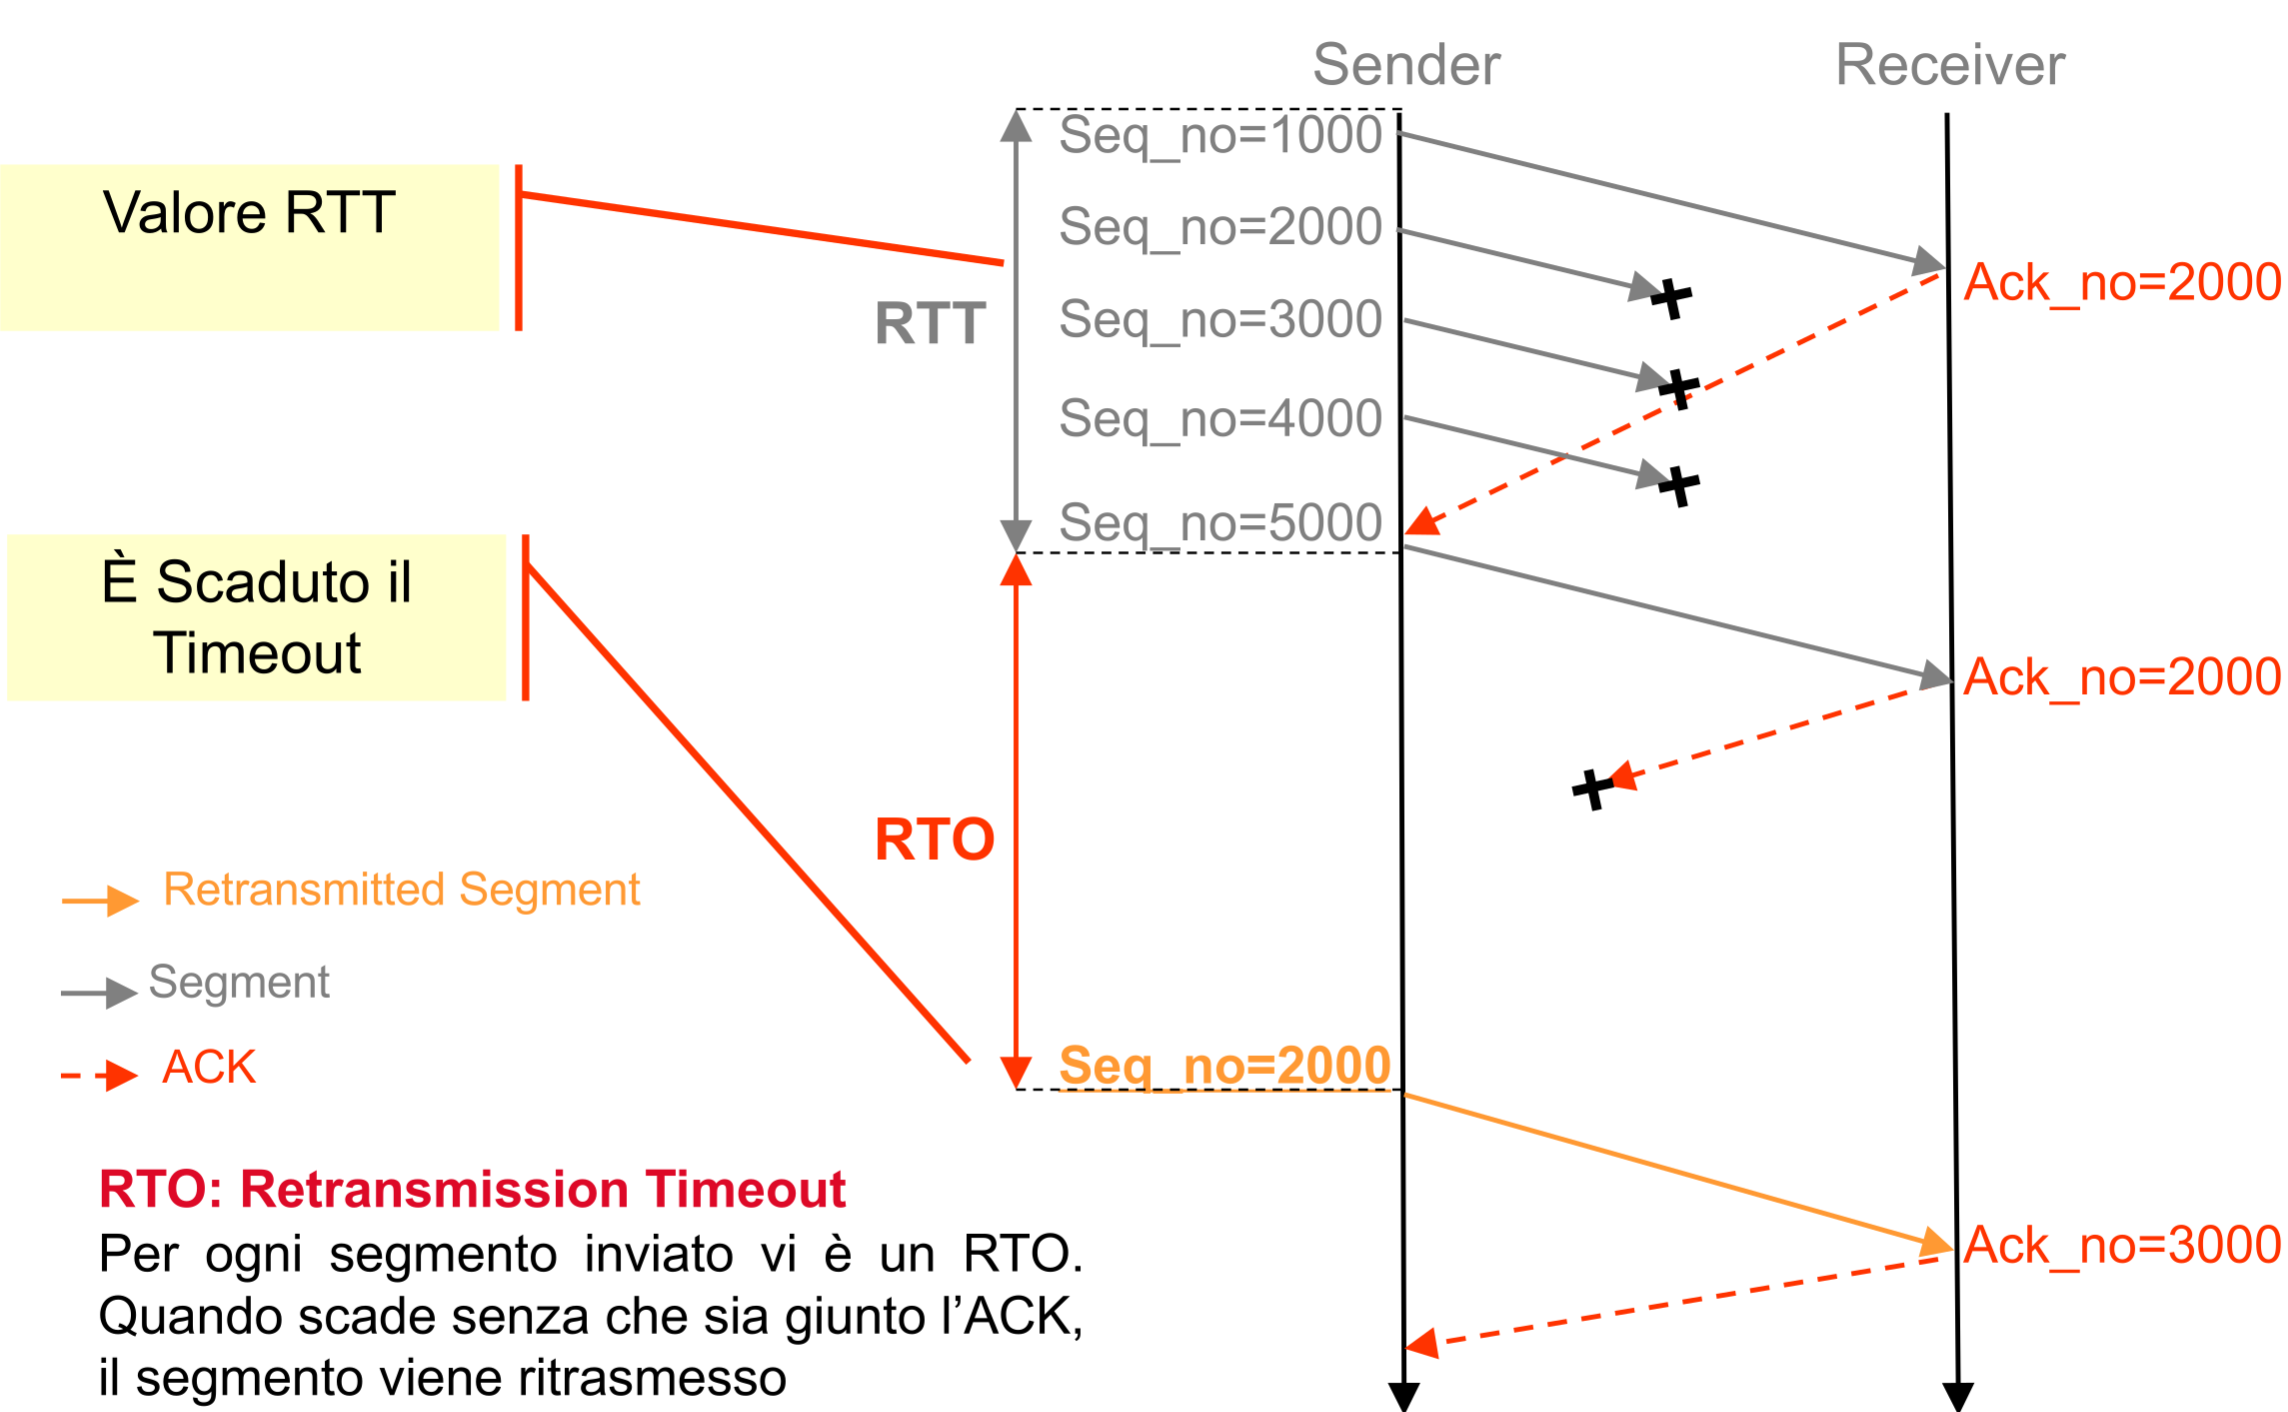
\includegraphics[width=0.9\textwidth]{images/rtotcp.png}
    \caption{Esempio di Retransmission Time Out (RTO) in TCP}
    \label{fig:rtotcp}
\end{figure}
Per ogni segmento inviato, viene avviato un RTO, ossia un timer che scade dopo un certo intervallo di tempo. Se il timer scade prima di ricevere l'ACK, il mittente ritrasmette il segmento.
\paragraph{Calcolo del RTO}



\newpage
\subsubsection{3 Dupack(three duplicate ACK)}
\begin{figure}[h!]
    \centering
    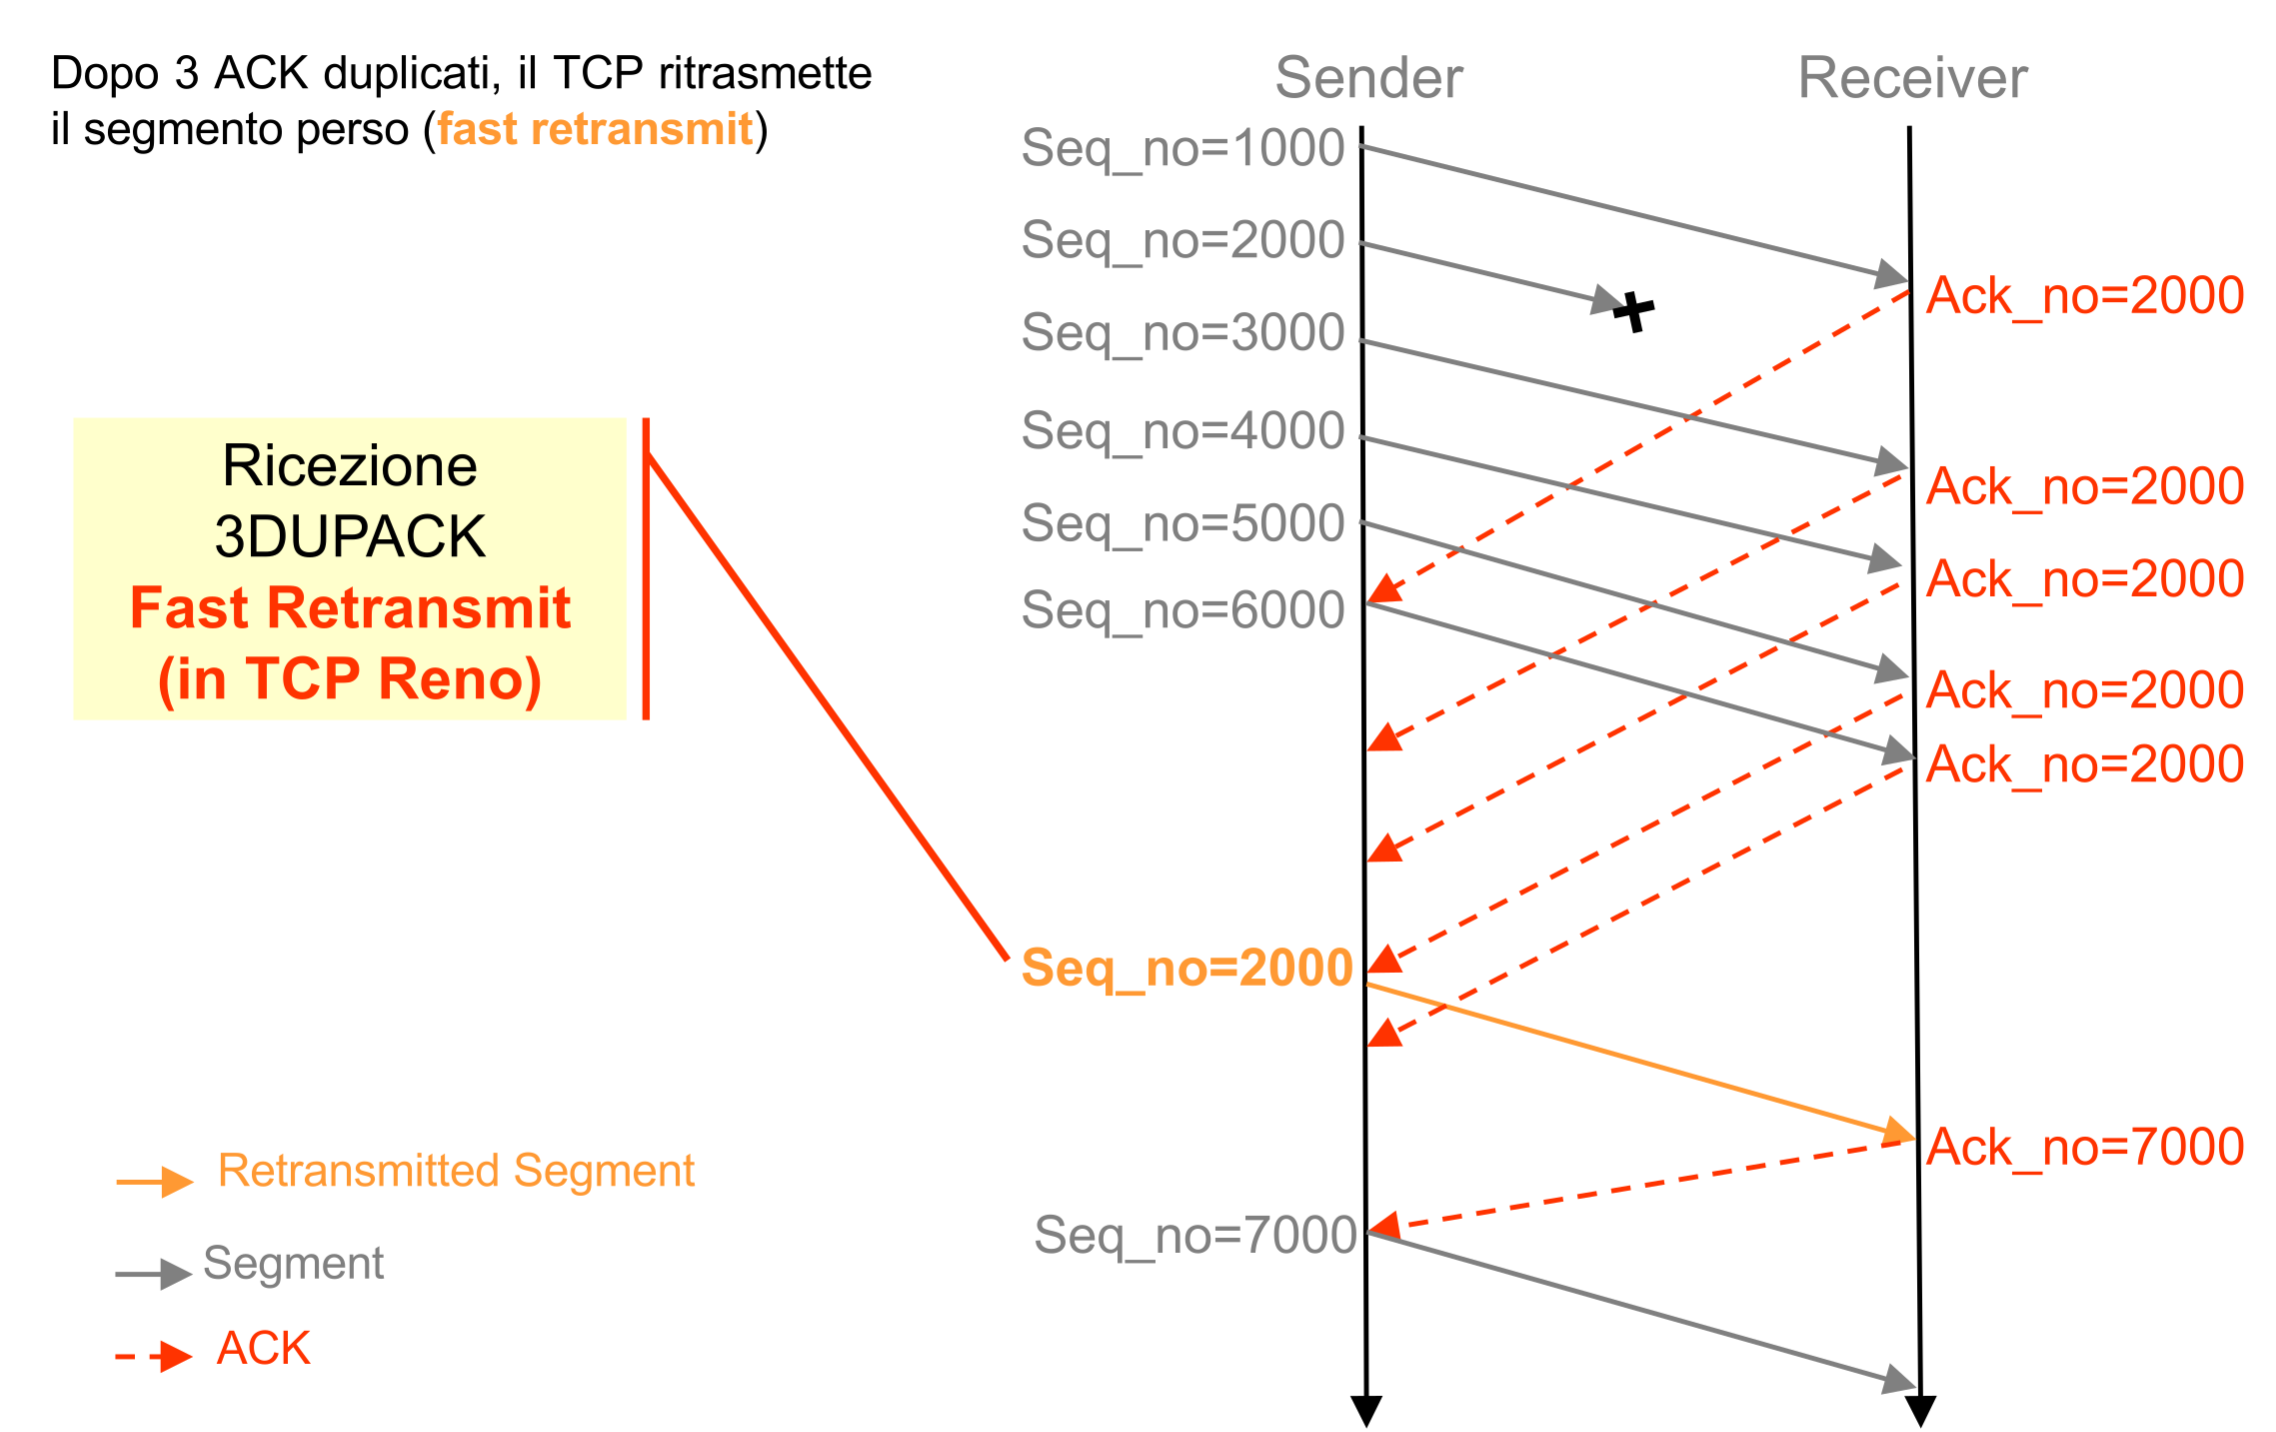
\includegraphics[width=0.8\textwidth]{images/3dupack.png}
    \caption{Esempio di 3 duplicate ACK (3 Dupack) in TCP}
    \label{fig:3dupack}
\end{figure}
\subsection{Controllo di congestione TCP}

I problemi di congestione si verificano quando la rete è sovraccarica(buff di ricezione saturo) di traffico e non riesce a gestire tutte le richieste. TCP utilizza diversi algoritmi per gestire la congestione e garantire una trasmissione affidabile dei dati.

Il protocollo TCP si rende conto dei limiti della rete solo quando avviene una congestione, quindi il TCP testa i limiti della rete(probing).

A tal scopo è importante definire le seguenti variabili:
\begin{itemize}
    \item rwnd(ricezione): è la dimensione della finestra di ricezione, ossia la quantità di dati che il mittente può inviare prima di ricevere un ACK dal destinatario.  
    \item cwnd(finestra di congestione): è dinamicamente calcolata tramite un algoritmo di controllo di congestione. 
\end{itemize}
\begin{figure}[h!]
    \begin{minipage}{0.45\textwidth}
        \centering
        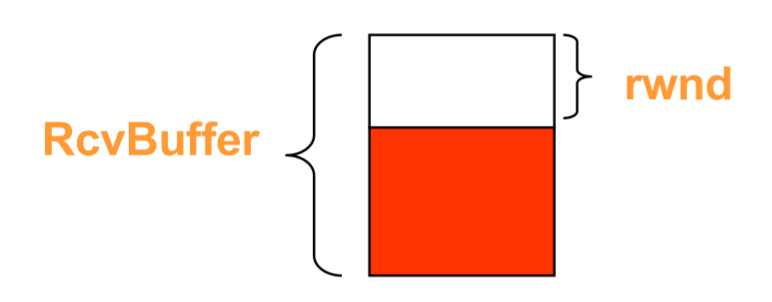
\includegraphics[width=\textwidth]{images/rwnd.png}
        \caption{Esempio di finestra di ricezione (rwnd) in TCP}
        \label{fig:rwnd}
    \end{minipage}
    \hfill
    \begin{minipage}{0.52\textwidth}
        \raggedright
        La finestra di trasmissione W è posta uguale al minimo tra la congestion window e la rwnd:
        \begin{equation}
            W = min(cwnd, rwnd)
        \end{equation}
        \raggedleft
    \end{minipage}
\end{figure}
Tramite la formula di W è possibile capire che questa finestra dipende da due variabili, una controllabile dal mittente(cwnd) ed una che dipende dal ricevente(rwnd).

La variabile cwnd ha il vantaggio di poter essere controllata, perciò se c'è una congestione in atto posso diminuire la variabile cwnd, modificando perciò la finestra di trasmissione W e la velocità di trasmissione, così da evitare di saturare la rete.

\subsubsection{Algoritmo di controllo di congestione}

\paragraph{Additive Increase Multiplicative Decrease (AIMD)}
TCP aumenta la finestra di ricezione aumentando "addittivamente" la cwnd. 
\paragraph{Probing}
Quando però avviene una congestione, la finestra non viene aumentata in modo additivo, ma anzi, viene ridotta drasticamente in modo moltiplicativo, moltiplicando la finestra per un fattore frazionario. 


\subsubsection{Evoluzione della cwnd}

        \paragraph{Slow start}
        Inizialmente la cwnd è pari ad 1 MSS, minimo valore possibile di cwnd, invia un segmento e inizia la fase di probing(slow start: parte "piano" per poi aumentare). Ogni volta che si ha un riscontro viene raddoppiata la cwnd. 

        \begin{itemize}
            \item MSS(maximum segment size): rappresenta la massima quantità di dati (in byte) che un host TCP può ricevere in un singolo segmento.
            tipicamnete 1460 byte (se MTU = 1500 e header IP+TCP = 40 byte)
            \item sstresh(slow star threshold): è una soglia che separa la fase di Slow Start da quella di Congestion Avoidance
        \end{itemize}

        Quando si verifica una congestione(3DUPACK o scadenza RTO), la cwnd e la soglia sshtresh(viene posta pari alla metà della finestra di congestione al momento della congestione) vengono modificate in base all'algoritmo di congestione utilizzato.

        \paragraph{Congestion avoidance}
        Nel caso in cui  la cwnd sia maggiore della soglia sshtresh, inizia la fase di congestion avoidance, in cui la cwnd viene aumentata linearmente, ossia viene incrementata di 1 MSS ogni RTT.

        L'obiettivo è quello di aumentare la cwnd in modo più lento, evitando di saturare la rete.
        \begin{equation}
            cwnd = cwnd + \frac{1}{\text{cwnd}}     \end{equation}
        
  
        \begin{figure}[h!]
        \centering
        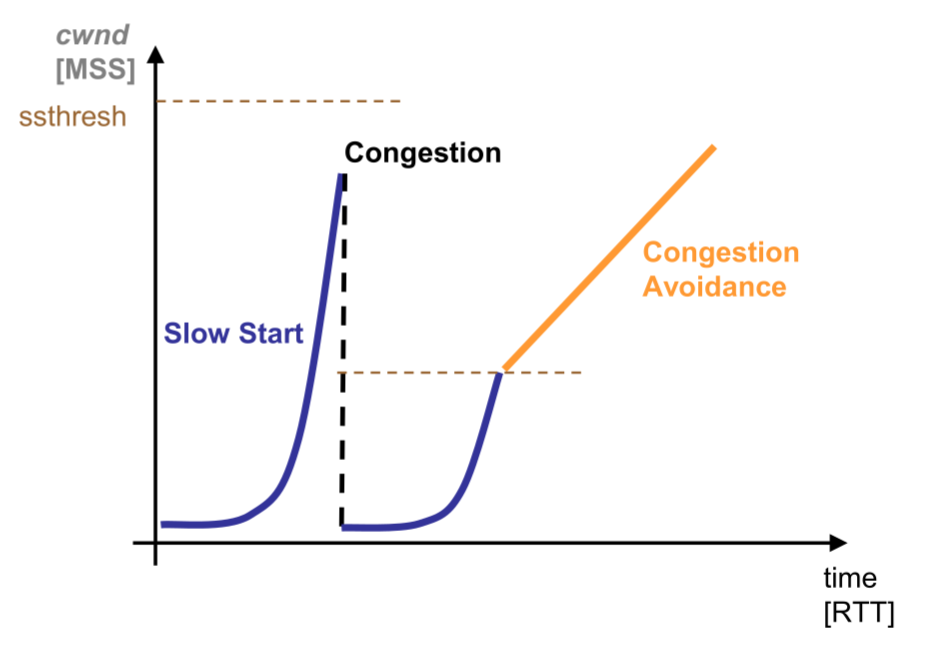
\includegraphics[width=0.7\textwidth]{images/graficocongestione.png}
        \caption{Andamento della finestra di congestione}
        \label{fig:graficocongestione}
        \end{figure}

        \newpage

\subsubsection{TCP Tahoe}

\begin{figure}[h!]
    \begin{minipage}{0.6\textwidth}
        \centering
        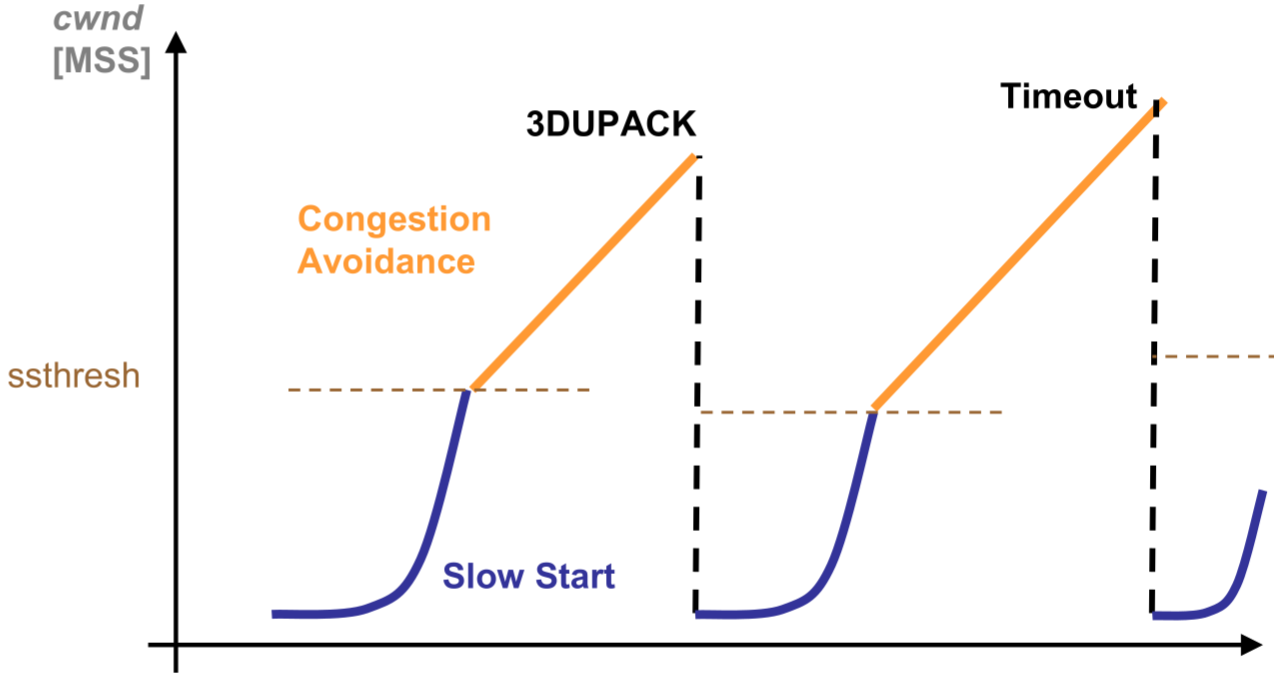
\includegraphics[width=0.95\textwidth]{images/tahoe.png}
        \caption{Andamento della finestra di congestione in Tahoe}
        \label{fig:tcptahoe}
    \end{minipage}
    \hfill
    \begin{minipage}{0.48\textwidth}
        TCP Tahoe non distingue tra i due eventi di congestione(3DUPACK e RTO), quando avviene riporta la cwnd a 1; rientrando in slow start.
    \end{minipage}
\end{figure}

\subsubsection{TCP Reno}

\begin{figure}[h!]
    \begin{minipage}{0.6\textwidth}
        \centering
        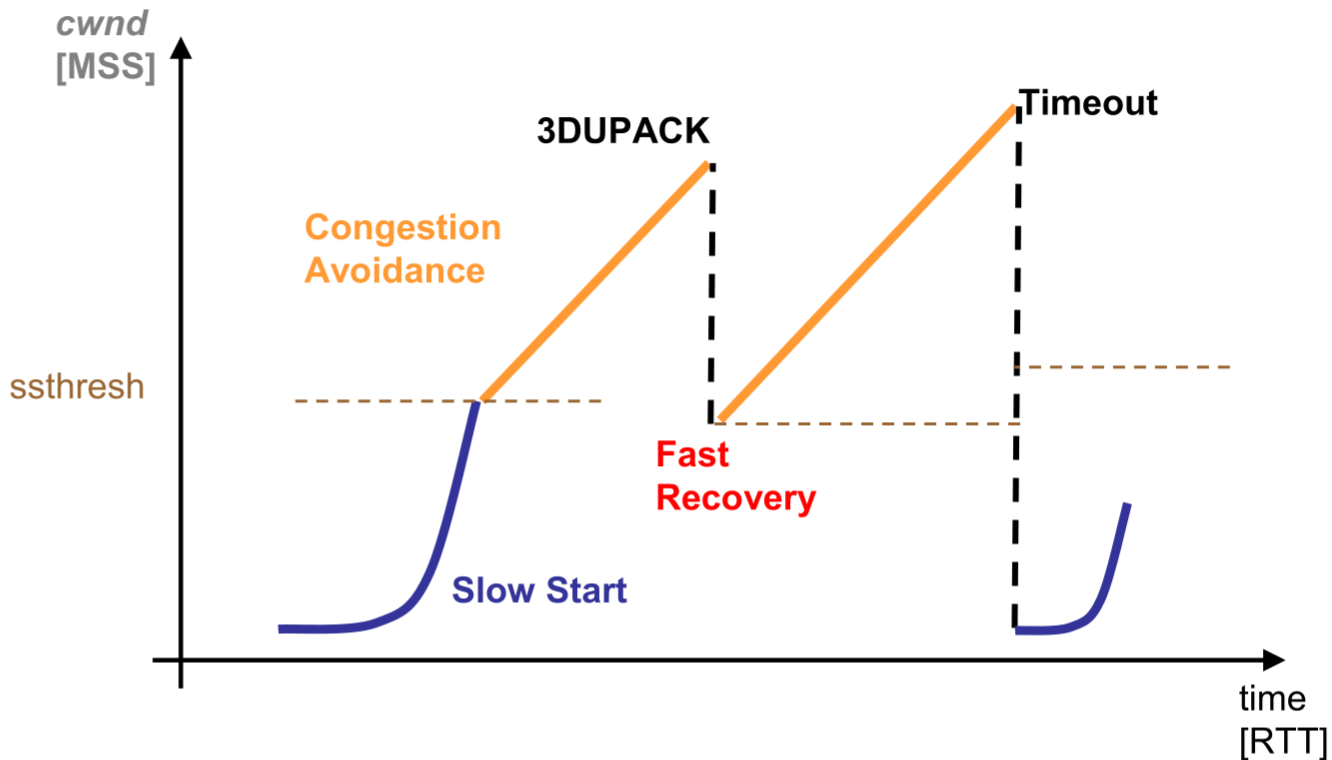
\includegraphics[width=0.95\textwidth]{images/reno.png}
        \caption{Andamento della finestra di congestione in Reno}
        \label{fig:tcpreno}
    \end{minipage}
    \hfill
    \begin{minipage}{0.48\textwidth}
        TCP Reno distingue i due eventi di congestione, (considerando che un 3DUPACK è un evento di congestione più "leggero" rispetto ad un RTO):
            \begin{itemize}
                \item In caso di 3DUPACK, la cwnd viene dimezzata e si entra nella fase di fast recovery, in cui la cwnd viene aumentata linearmente fino a raggiungere la soglia sshtresh.
                \item In caso di RTO, la cwnd viene riportata a 1 e si entra nella fase di slow start.
            \end{itemize}   
    \end{minipage}
\end{figure}

\subsubsection{TCP New Reno}

\begin{figure}[h!]
    \begin{minipage}{0.6\textwidth}
        \centering
        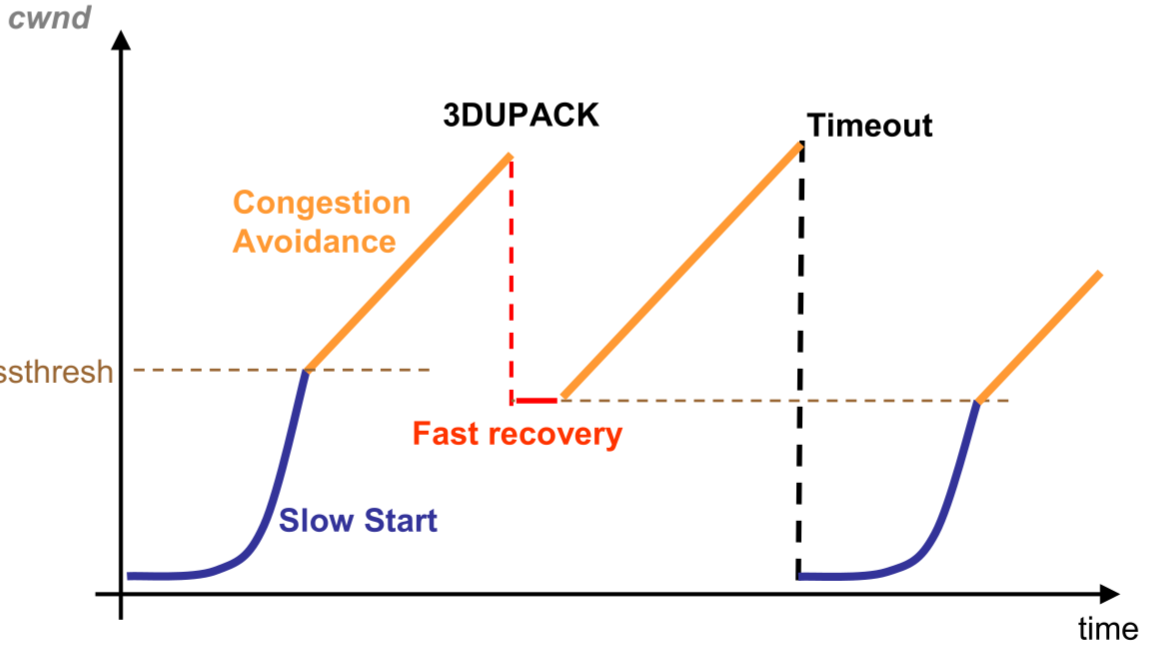
\includegraphics[width=0.95\textwidth]{images/newreno.png}
        \caption{Andamento della finestra di cong. in New Reno}
        \label{fig:tcpnewreno}
    \end{minipage}
    \hfill
    \begin{minipage}{0.48\textwidth}
        Nel reno visto in precedenza ad ogni 3DUPACK viene dimezzata la cwnd, ma questo non è ottimale nel caso in cui avvengano più 3DUPACK nella stessa finestra.

        Perciò esiste la variante New Reno, che non dimezza la cwnd ad ogni 3DUPACK, lo fa solamente la prima volta che avviene all'interno della finestra; quelli successivi vengono ignorati.
    \end{minipage}
\end{figure}
%piggybacking

%\chapter{Livello 3 rete}
%\section{Internet Protocol (IP) version 4}

\subsection{Introduzione}
\begin{figure}[h!]
    \begin{minipage}{0.45\textwidth}
        \centering
        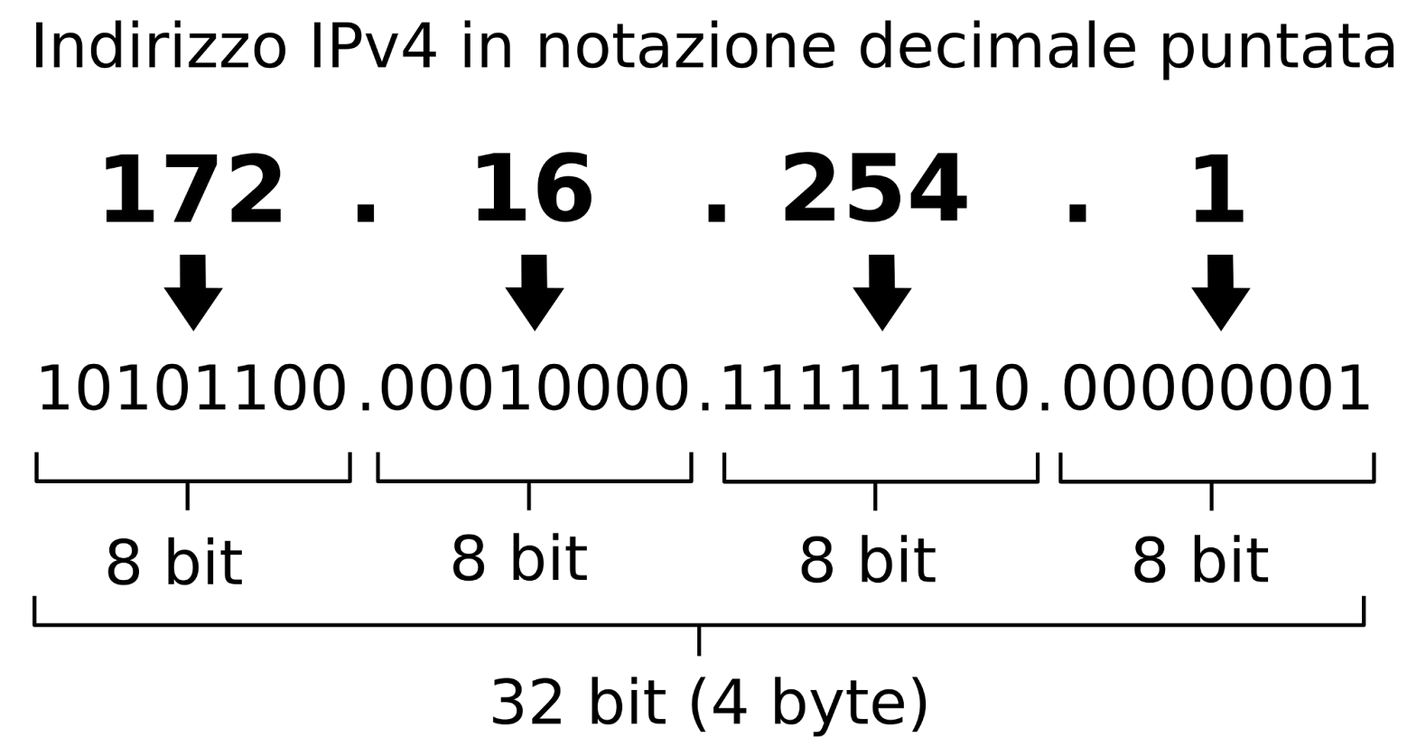
\includegraphics[width=0.95\textwidth]{images/indirizzoip.png}
        \caption{Struttura di un indirizzo IP}
        \label{fig:indirizzoip}
    \end{minipage}\hfill
    \begin{minipage}{0.52\textwidth}
        Al livello 3 ci preoccupiamo di trovare la strada migliore per raggiungere il destinatario.

        IPv4 è il protocollo di rete più diffuso al mondo, IP instrada i pacchetti immessi nella rete, ogni nodo in rete ha indirizzo ip.

        Ogni pdu(pacchetto) contiene gli indirizzi IP del host mittente e destinatario.
        
        IP è connectionless, ad inoltrare i pacchetti(datagram) sono i router, lo fanno attraverso algoritmi di routing(leggendo l’header del pacchetto). 

        Ip è inoltre “best-effort”, ossia fa del suo meglio, non garantisce affidabilità massima o ottimale.

        Gli indirizzi ip sono da 32 bit(4 numeri decimali compresi tra 0 e 255):
    \end{minipage}
\end{figure}

Gli host che appartengono alla stessa rete hanno in comune il livello fisico,
un dominio di broadcast è un insieme di computer di una stessa rete(stesso indirizzo ip di rete), esempio rete di casa(collegandoci al router di casa è possibile inviare un messaggio broadcast che arriverà a tutti i dispositivi che fanno parte della rete IP).
Le porte del router vengono chiamate interfacce, ogni interfaccia corrisponde ad un host;
ogni rete ha un indirizzo IP di rete.

\begin{figure}[h!]
    \centering
    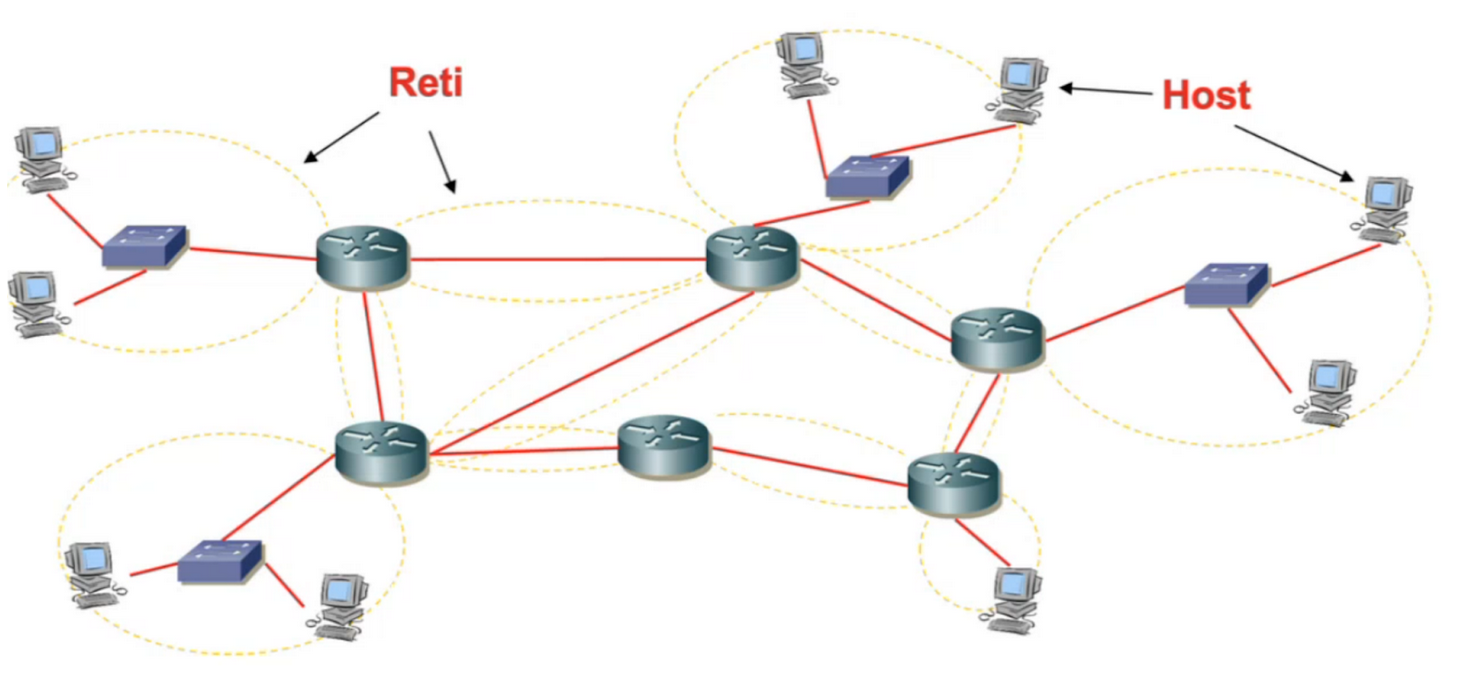
\includegraphics[width=0.59\textwidth]{images/reteipbase.png}
    \caption{Esempio di rete IP di base}
    \label{fig:reteipbase}
\end{figure}
\subsection{Datagramma IP}
I datagrams IP sono i pacchetti di dati che vengono inviati attraverso la rete utilizzando il protocollo IP. Ogni datagramma contiene un header e un payload. 
\begin{figure}[h!]
    \centering
    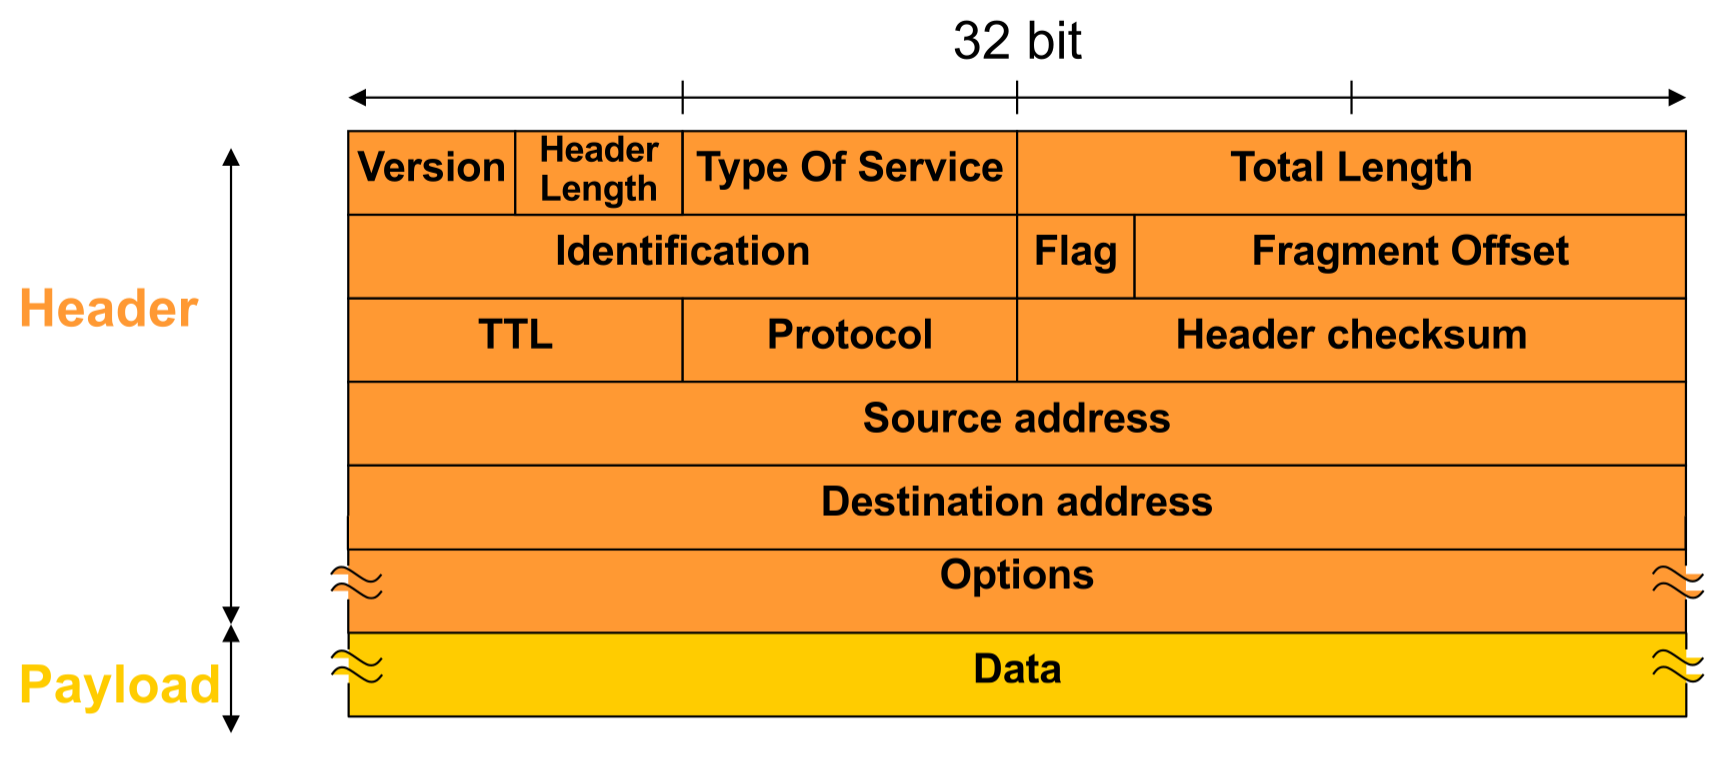
\includegraphics[width=0.9\textwidth]{images/datagrammaIP.png}
    \caption{Struttura di un datagramma IP}
    \label{fig:datagrammaIP}
\end{figure}

\begin{itemize}
    \item version: mi dice la versione del protocollo(IPv4 o IPv6) (è di 4 bit, mezzo byte)
    \item header legth: lunghezza del header (4 bit, mezzo byte), se voglio dire che l'header è lungo 5 posso scivere in questo campo 0101, che è 1 + 0 + 4 + 0
    \item type of service(TOS): (1 byte, 8 bit) distingue i tipi diversi di pacchetti, questo è utile nel momento in cui un router deve dare o no la precedenza a certi pacchetti, in base al tipo di servizio. esempio: precedenza al servizio x piuttosto che a y
    il TOS viene utilizzato per definire il liello di quality of service con cui trattare il pacchetto(primi 6 bit)(gli ultimi 2 servono ad evitare la congestione)
    
    \begin{figure}[h!]
        \centering
        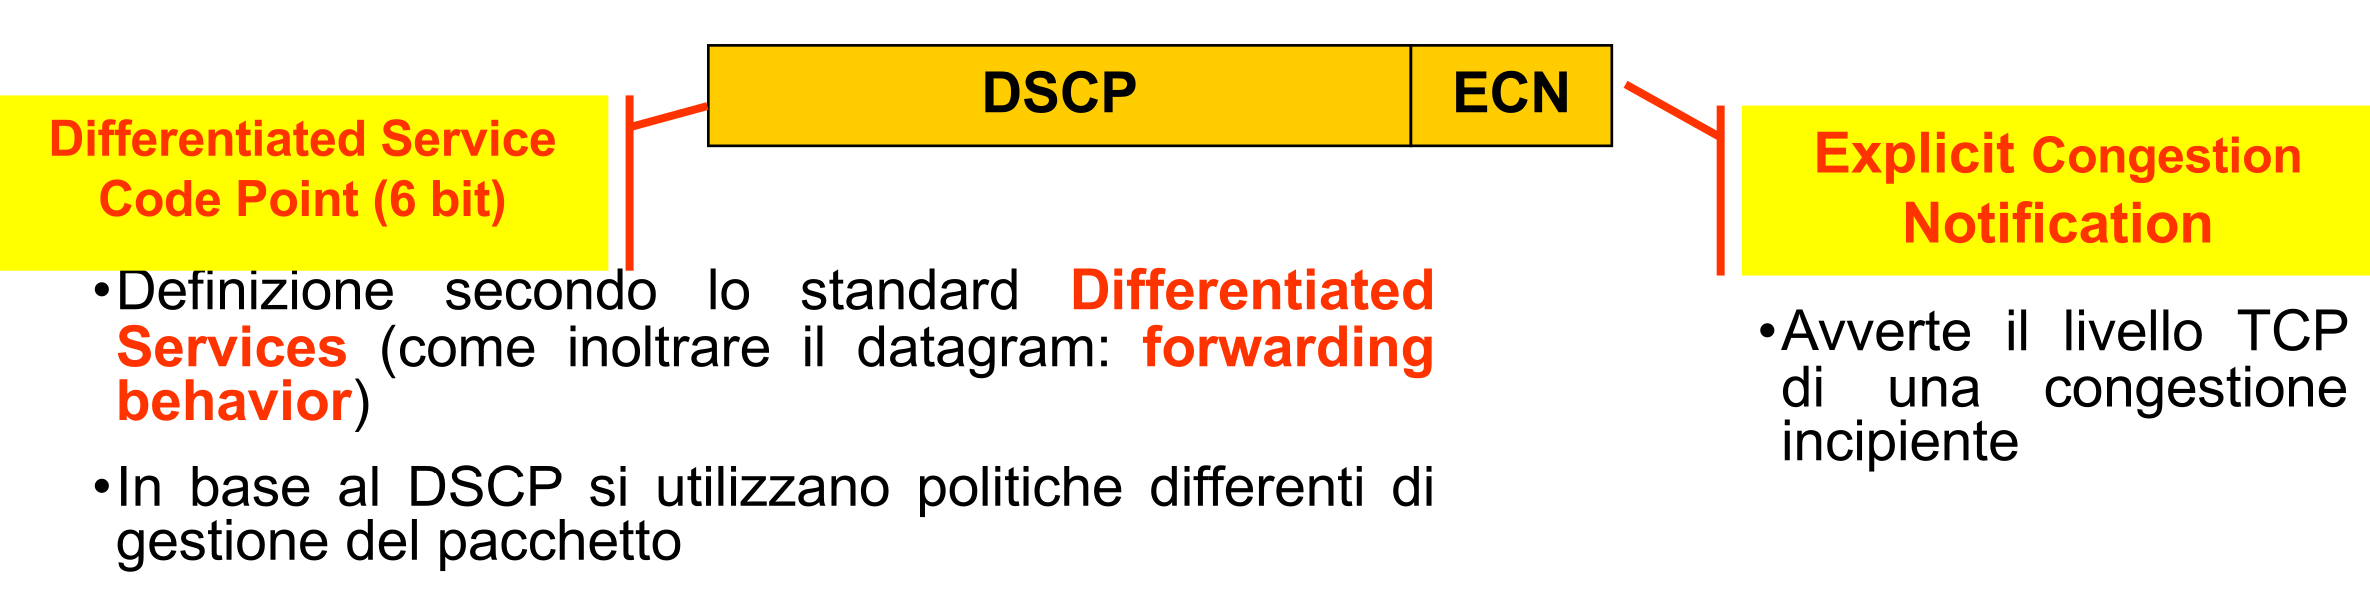
\includegraphics[width=1\textwidth]{images/tos.png}
        \caption{Campo Type of Service (ToS) nell'header IP}
        \label{fig:tos}
    \end{figure}

    \item total length:(16 bit) lunghezza del datagramma in byte(max 65535 byte)
    \item identification(16 bit) identifica in modo univoco un datagramma generato dal mittente, quindi anche se il pacchetto viene frammentato, i suoi “frammenti”, ossia altri pacchetti che contengono parte del payload iniziale, avranno lo stesso id. serve quindi a gestire la frammentazione dei pacchetti ip
    \item options: opzioni per il routing del pacchetto, è un campo poco usato per via del carico di elaborazione molto variabile
    \item data: è l'informazione da inviare
\end{itemize}
\newpage
\begin{itemize}
    \item flag(3 bit)
\end{itemize}
        \begin{figure}[h!]
            \begin{minipage}{0.55\textwidth}
                \raggedright
                 il primo bit non usato, il secondo bit è il flag DF (don't fragment: specifica che il router può frammentare il pacchetto o no), il terzo bit è il flag MF (more fragment: indica se il seguente datagramma è l'ultimo dei frammenti). Per utilizzare questi flag metto il valore del bit corrispondente al flag ad 1. Esempio: 010, 0 iniziale è indifferente, 1 indica il flag DF attivo, mentre lo 0 alla fine mi dice che non è MF, quindi che questo datagram è l'ultimo frammento.
            \end{minipage}\hfill
            \begin{minipage}{0.4\textwidth}
                \centering
                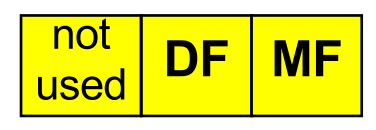
\includegraphics[width=\textwidth]{images/flagsIP.png}
                \caption{Campo Flags nell'header IP}
                \label{fig:flagsIP}
            \end{minipage}
        \end{figure}
\begin{itemize}
    \item fragment offset(13 bit) mi dice la posizione del frammento all'interno del pacchetto originario, lo spiazzamento. è espresso in multipli di 8 byte. 
\end{itemize}

    \begin{figure}[h!]
        \begin{minipage}{0.55\textwidth}
            \textbf{Frammentazione}: quando un datagramma IP deve attraversare una rete con una MTU (Maximum Transmission Unit) inferiore alla sua dimensione, viene suddiviso in frammenti più piccoli. Ogni frammento contiene parte dei dati originali e un header IP con informazioni per il riassemblaggio.

            Nella figura il pacchetto è grande 4000 byte(total length), in questo caso viene frammentato in 3 poichè la sua MTU vale 1500 byte , i frammenti condividono lo stesso id del pacchetto non frammentato.

            I frammenti devono avere un offset multiplo di 8.

            Solamente il primo frammento ha offset pari a 0, rappresenta la testa.
            Solamente l'ultimo frammento ha MF pari a 0 poichè sta ad indicare che quello è l'ultimo pezzo del pacchetto, la coda. CHIARIRE
        \end{minipage}\hfill
        \begin{minipage}{0.4\textwidth}
            \centering
            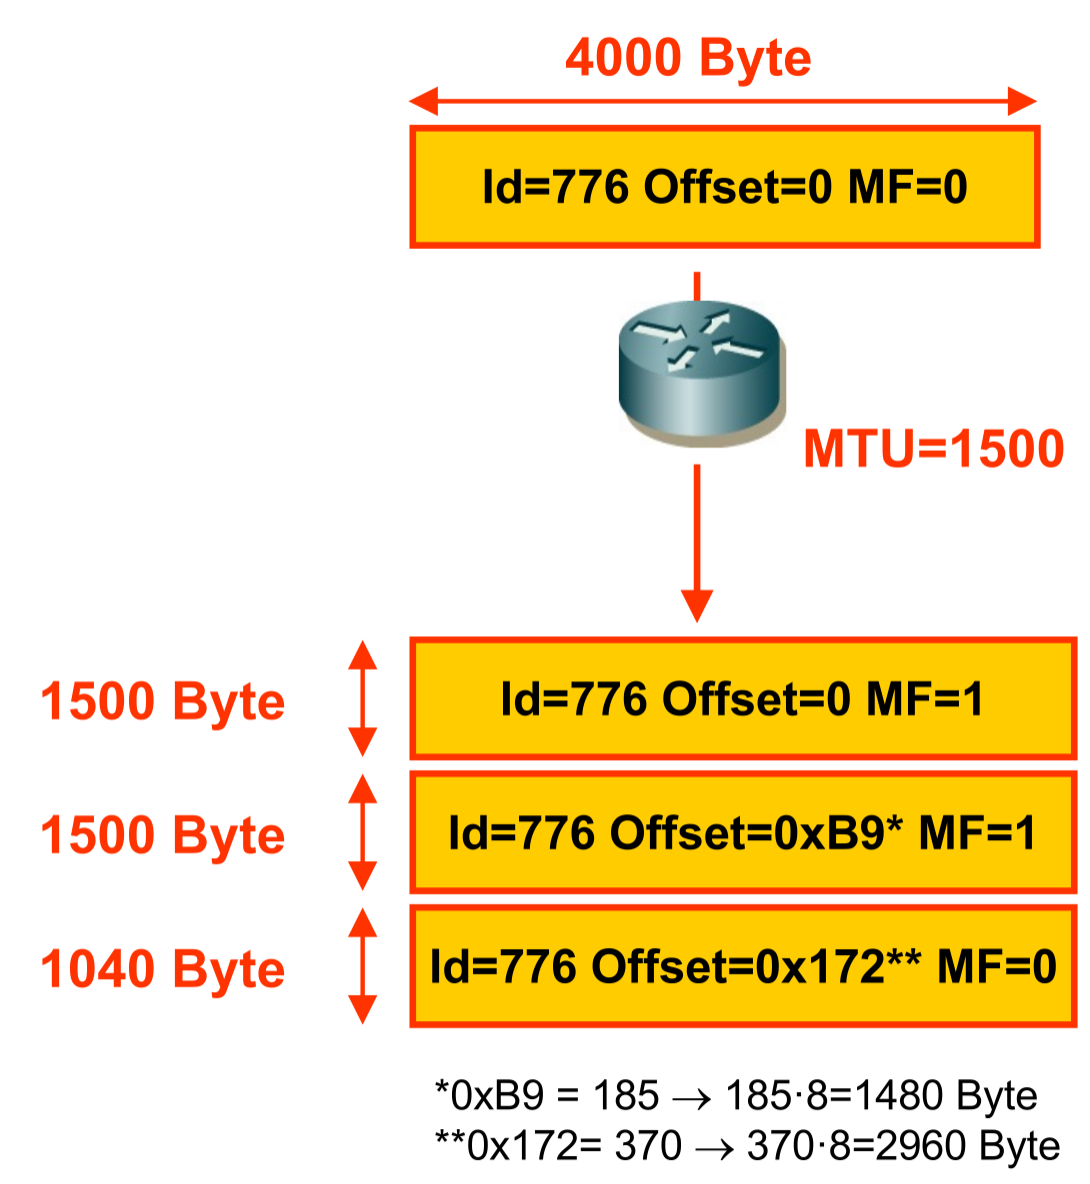
\includegraphics[width=\textwidth]{images/frammentazione.png}
            \caption{Esempio di frammentazione di un datagramma IP}
            \label{fig:frammentazioneIP}
        \end{minipage}
    \end{figure}

\begin{itemize}
    \item time to live(8 bit) evita il problema dei pacchetti che entrano in loop poichè non trovano il destinatario. è il tempo di vita del pacchetto, ogni router che riceve il pacchetto(ad ogni hop) decrementa il valore time to live, facendo così arriverà un punto in cui il time to live del pacchetto è stato decrementato fino a zero. quando arriva a 0 il datagram viene scartato. è un valore stabilito dal mittente(esempio 128)
    \item protocol(8 bit): contiene un numero che specifica il protocollo usato dalla PDU incapsulata dal datagram. esempio TCP = 6 . UDP = 17 $\rightarrow$ livello 4
    \item header checksum(16 bit): controlla i byte del header, è un controllo veloce su header. se c'è un errore sull'header allora il pacchetto viene scartato, come funziona? : somma 16 bit a 16 bit gli altri byte dell’header,fa la somma dell'eventuale resto e fa il complemento ad 1 del risultato.

Se non ci sono errori, la somma a 16 bit di tutti questi valori deve dare come risultato 0xFFFF (cioè tutti i bit a 1).

\item source/destination address: (32 bit) è l'indirizzo ip del mittente/destinatario

\end{itemize}

\subsubsection{Struttura indirizzo IP}
\begin{figure}[h!]
    \centering
    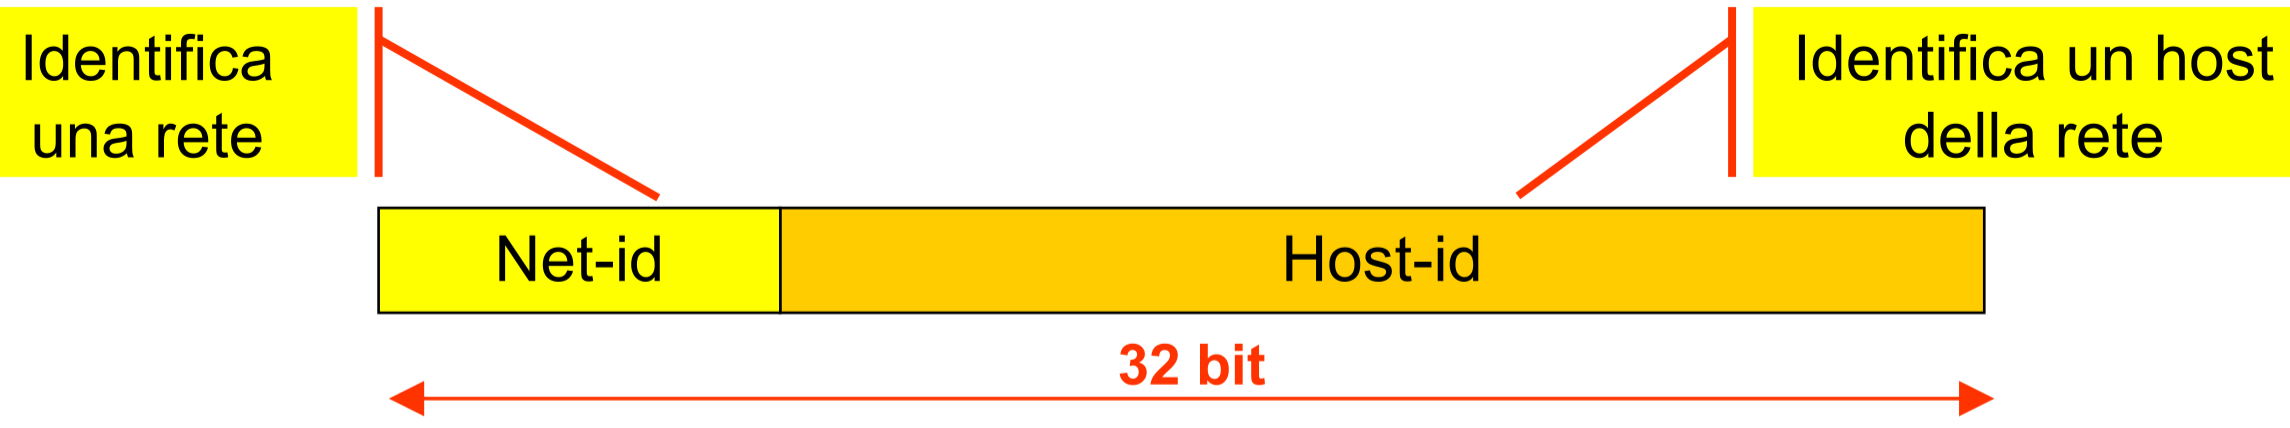
\includegraphics[width=0.8\textwidth]{images/strutturaIP.png}
    \caption{Struttura di un indirizzo IP: suddivisione in parte di rete e parte host}
    \label{fig:strutturaIP}
\end{figure}

Attualmente si utilizza l'indirizzamento classless CIDR (Classless Inter-Domain Routing), che permette di specificare la lunghezza della maschera di rete in bit.

L'assegnazione degli indirizzi è compito dell'Internet Assigned Number
Authority (IANA) gestita dall'ICANN (Internet Corporation for Assigned
Names and Numbers).

Ogni interfaccia (host) della rete IP ha un suo indirizzo.

\subsection{Indirizzo IP - classful}

\begin{figure}[h!]
    \centering
    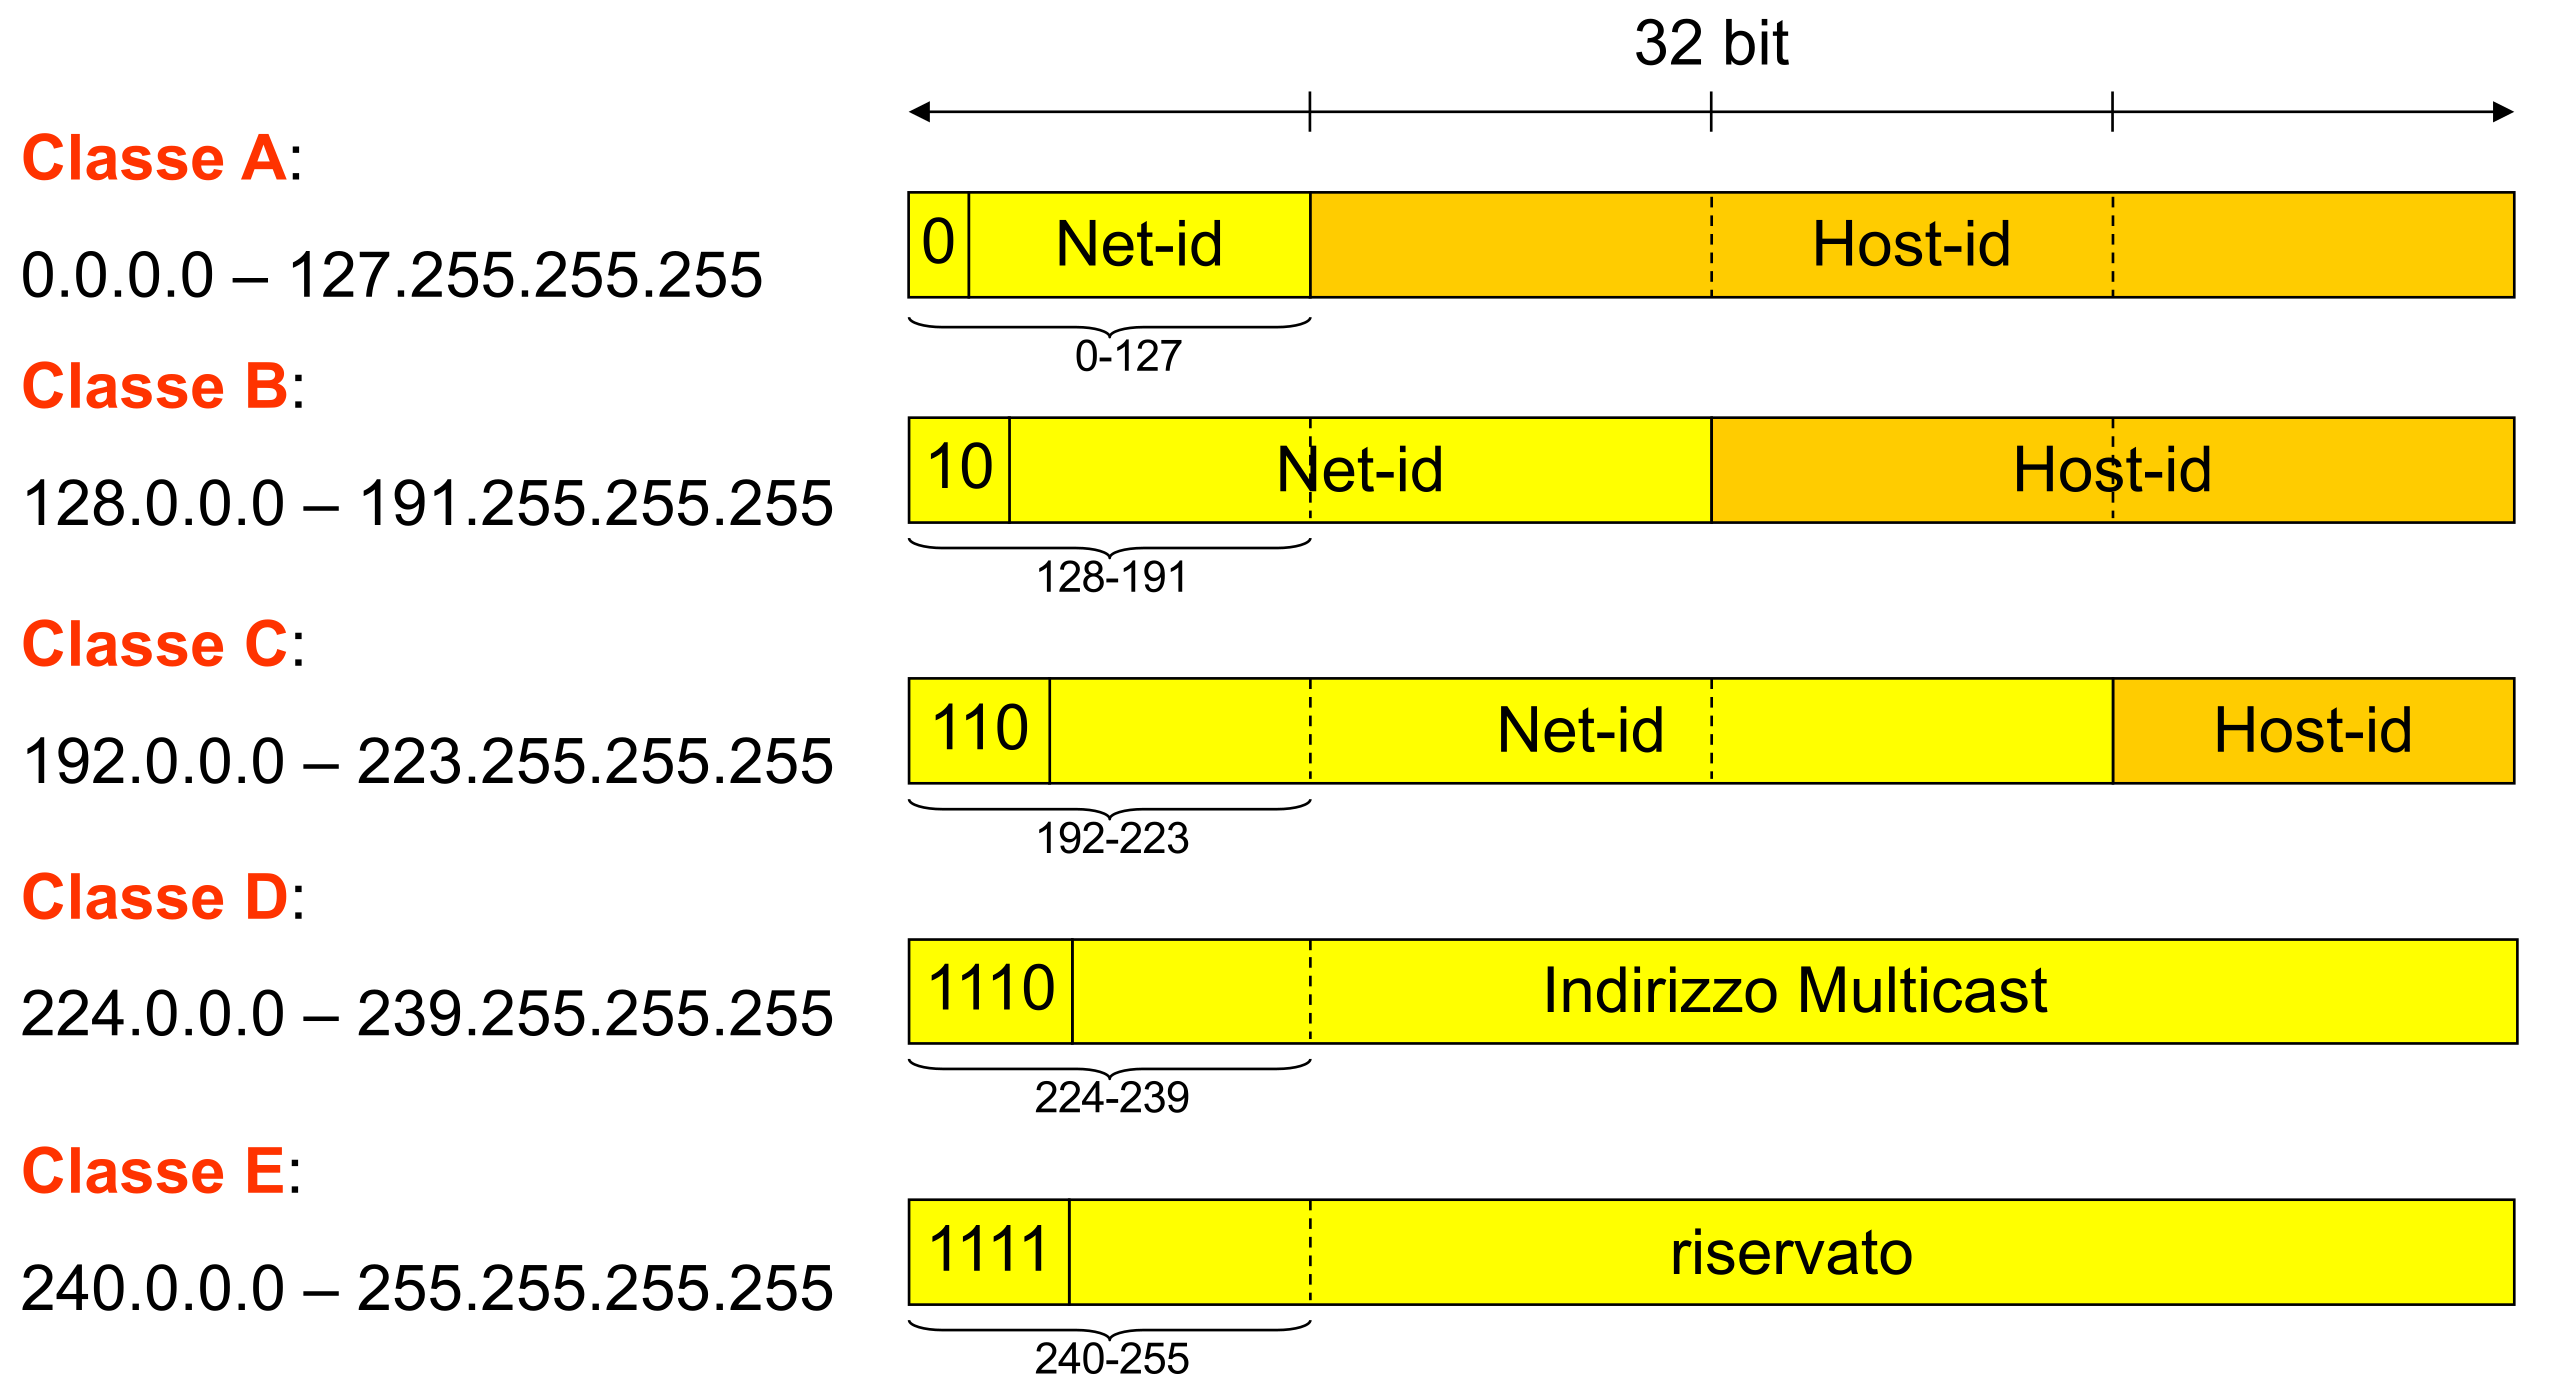
\includegraphics[width=1\textwidth]{images/classfulladdressing.png}
    \caption{Classful Addressing: suddivisione degli indirizzi IP in classi A, B, C, D, E}
    \label{fig:classfuladdressing}
\end{figure}

\subsection{Indirizzo IP - classless CIDR}

\begin{figure}[h!]
    \begin{minipage}{0.45\textwidth}
        \centering
        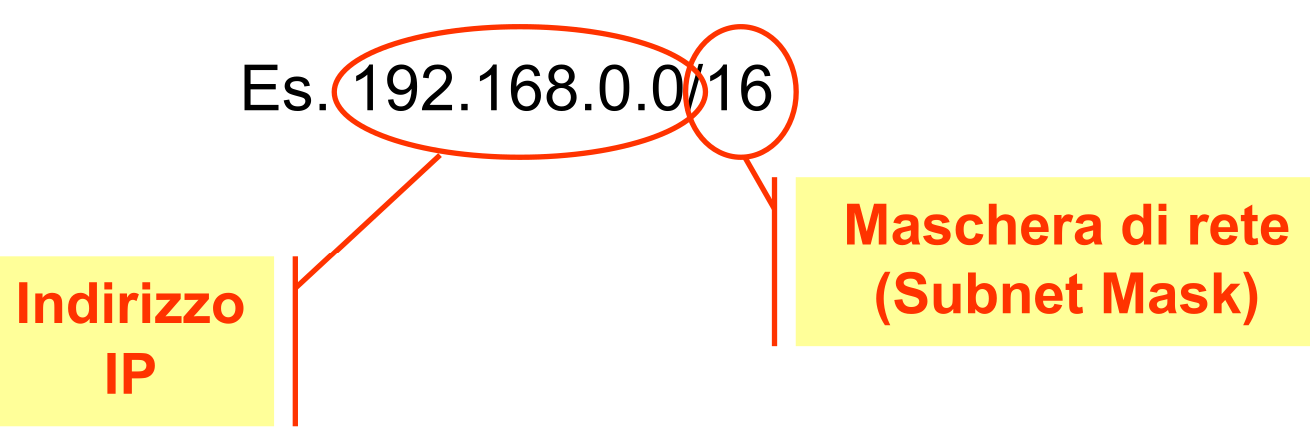
\includegraphics[width=0.95\textwidth]{images/mascheraIP.png}
        \caption{Esempio di maschera di rete (netmask) in notazione decimale e binaria}
        \label{fig:mascheraIP}
    \end{minipage}\hfill
    \begin{minipage}{0.52\textwidth}
        Il formato dell'indirizzo è del tipo \texttt{a.b.c.d/x} dove $x$ rappresenta la lunghezza della maschera di rete in bit.

        La maschera di rete permette di distinguere la parte di indirizzo relativa alla rete da quella relativa all'host. In notazione CIDR, la maschera viene indicata dopo una barra, ad esempio \texttt{192.168.1.0/24}.
    \end{minipage}
\end{figure}

\paragraph{Riconoscere un indirizzo di rete e un indirizzo di host}

Per riconoscere un indirizzo di rete e un indirizzo di host, si utilizza la maschera di rete. La maschera di rete è un numero che indica quanti bit dell'indirizzo IP sono dedicati alla parte di rete e quanti alla parte di host.

\begin{itemize}
    \item Un indirizzo di rete ha tutti zero nella parte di host.
\end{itemize}
\subsection{Subnetting}


\subsection{Classificazione degli indirizzi IP}

\subsubsection{Pubblici}
\subsubsection{Privati}

\subsubsection{Statici}
\subsubsection{Dinamici}


\subsection{Variable Length Subnet Mask (VLSM)}
\subsection{Indirizzi IP speciali}

\begin{figure}[h!]
    \centering
    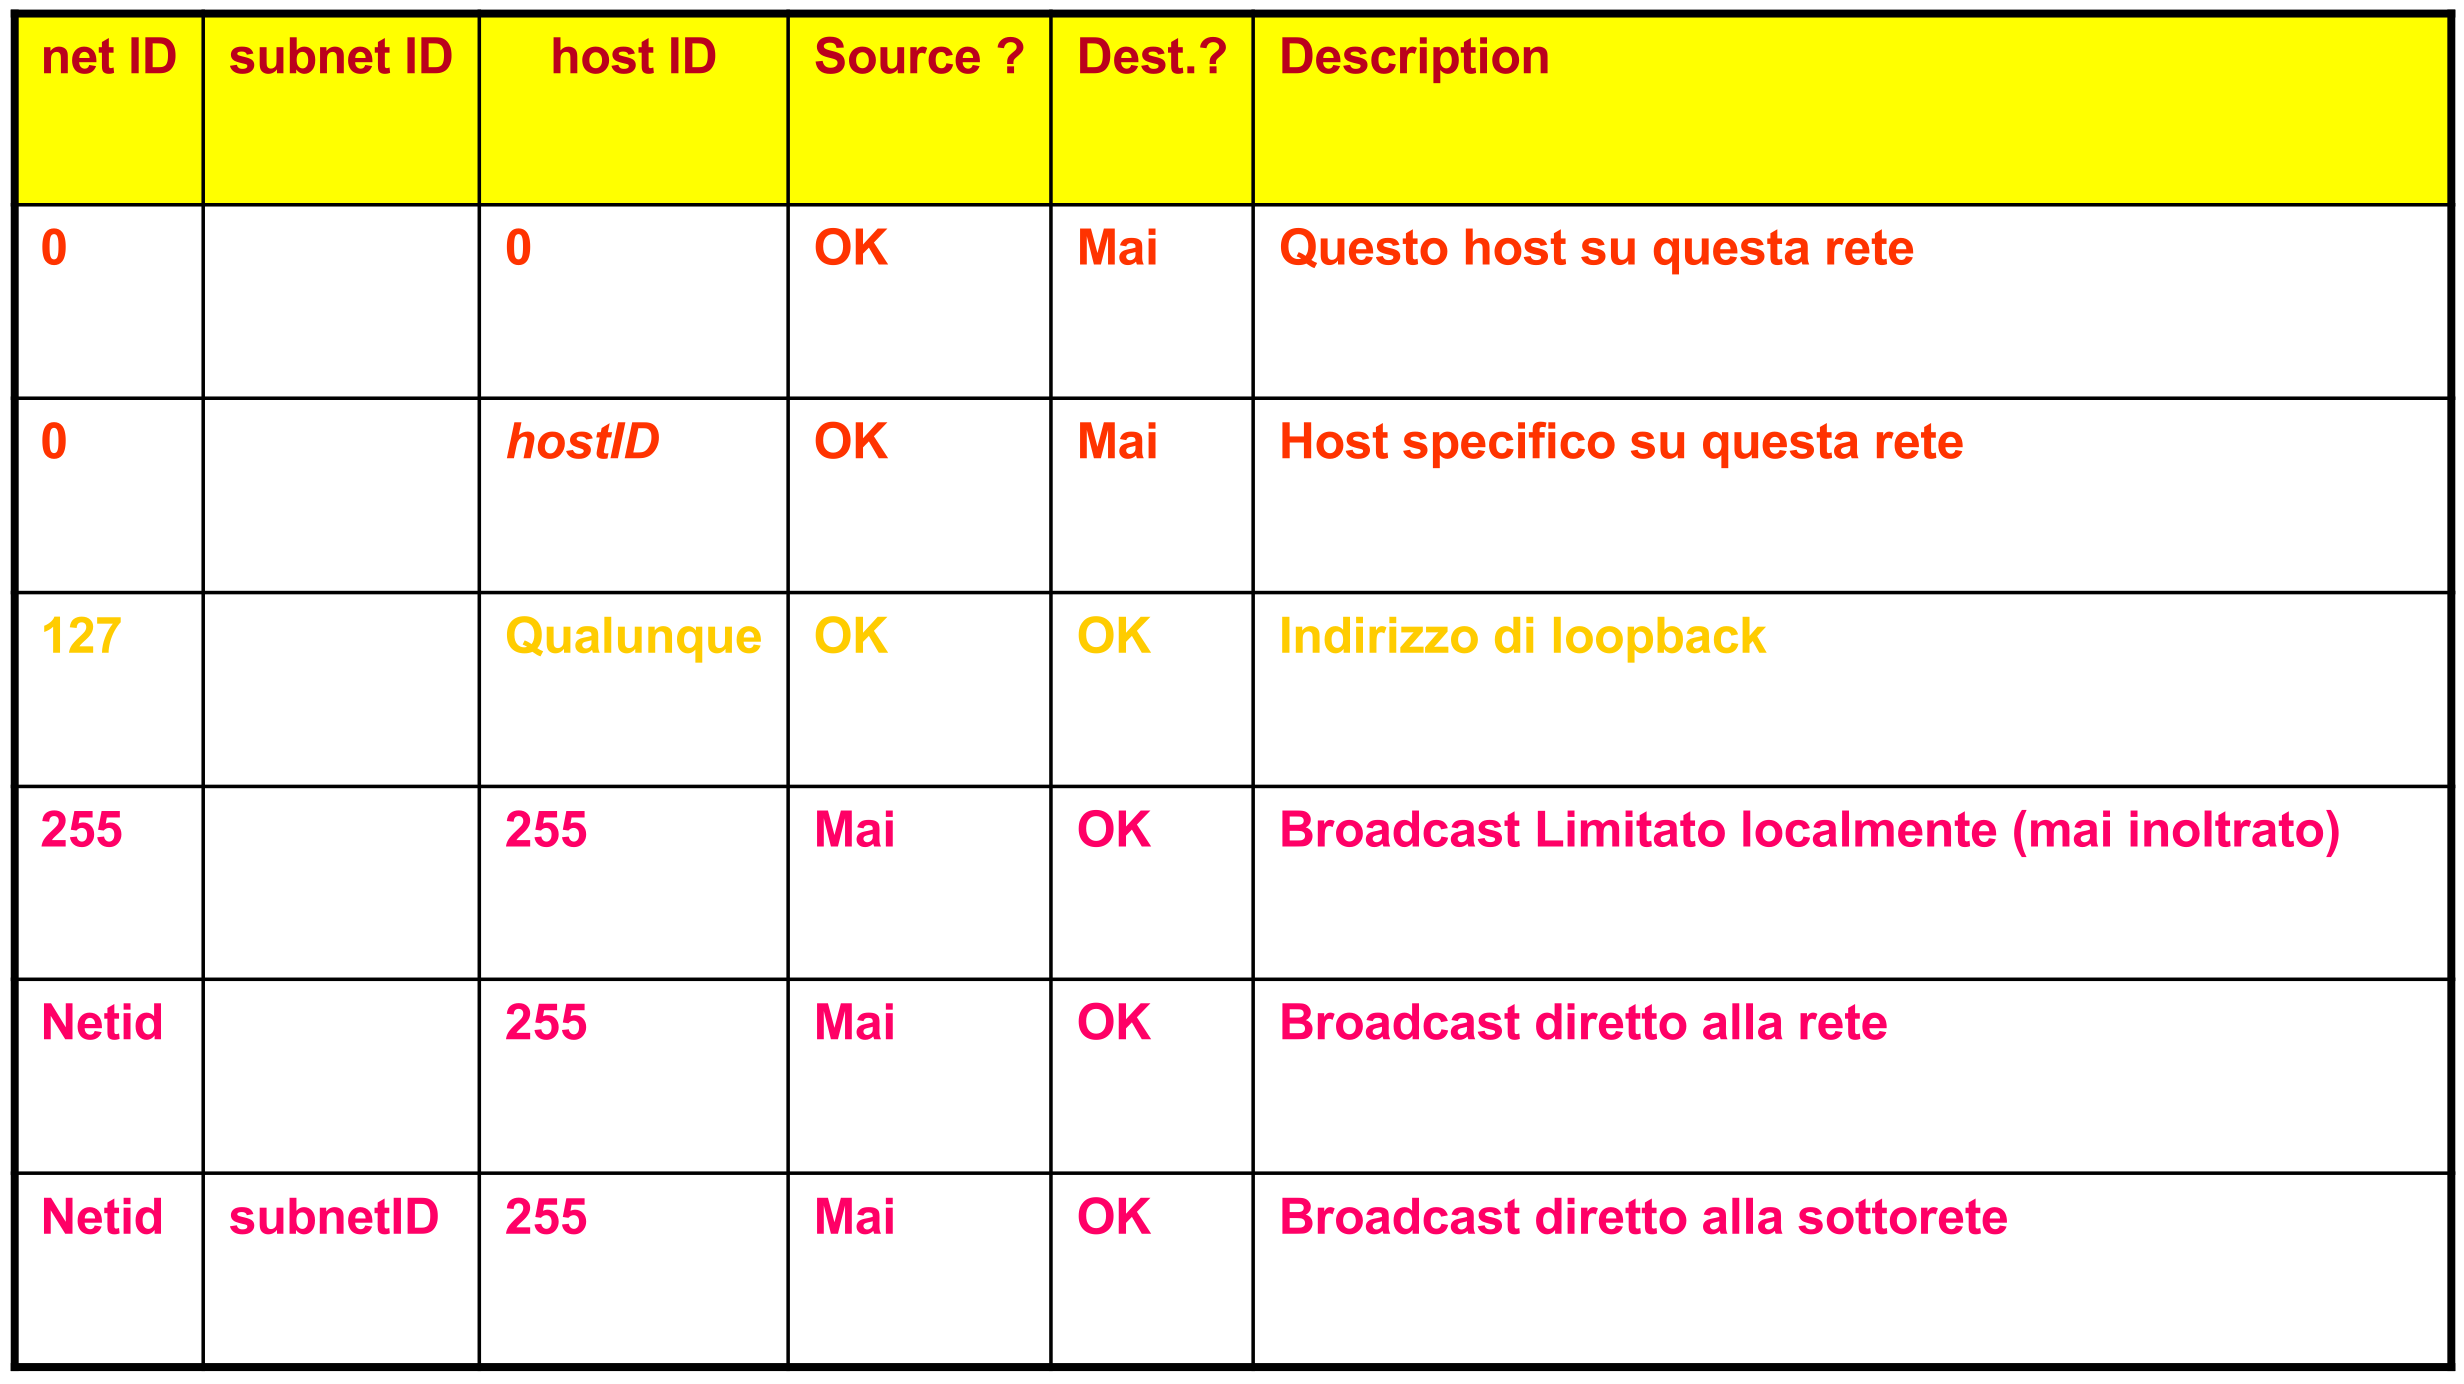
\includegraphics[width=1\textwidth]{images/indirizziipspeciali.png}
    \caption{Indirizzi IP speciali}
    \label{fig:indirizziipspeciali}
\end{figure}


\newpage
\subsection{Address Resolution Protocol (ARP) - mappatura IP a MAC}
Con ART si intende un protocollo di rete appartenente alla suite del protocollo internet (IP) versione 4 e operante a livello di accesso alla rete (livello collegamento se si considera nomenclatura ISO/OSI), il cui compito è fornire la "mappatura" tra l'indirizzo IP (32 bit - 4 byte) e l'indirizzo MAC (48 bit - 6 byte) corrispondente di un terminale in una rete locale ethernet.

Cos'è l'indirizzo MAC? 

Un indirizzo MAC (dove MAC sta per Media Access Control), detto anche "indirizzo fisico" o "indirizzo Ethernet", è un codice di 48 bit associato ad ogni dispositivo di rete che implementa lo standard Ethernet. Il suo scopo principale è quello di attribuire un'identità univoca a ciascuno dei nodi collegati ad uno stesso segmento di rete, consentendo quindi comunicazioni locali di tipo unicast. 

Al Livello 2 del modello ibrido, i pacchetti viaggiano attraverso il collegamento di più nodi, questi nodi sono caratterizzati da indirizzi fisici detti mac. 
Invece a livello tre l'indirizzo che possiede il pacchetto è !l'indirizzo definitivo!(il destinatario, non i nodi intermedi), la meta ultima del pacchetto. Però questi pacchetti viaggiano attraverso dei nodi, quindi a livello 2 i pacchetti avranno come destinazioni i nodi, e per raggiungerli hanno bisogno di conoscere gli indirizzi fisici dei nodi, perciò tramite gli indirizzi MAC e il protocollo arp si risolve il problema locale del collegamento tra i vari nodi che fanno si che il pacchetto viaggi attraverso quelli.

ARP risponde quindi a questa domanda: ho questo indirizzo ip, mi dici quale sia l'indirizzo di livello due corrispondente a questo ind ip??

Mi dice l'indirizzo del “prossimo nodo”, livello 2.

Quindi un protocollo fondamentale che individua da un indirizzo ip(liv 3) uno o più di livello 2


\begin{figure}[h!]
    \centering
    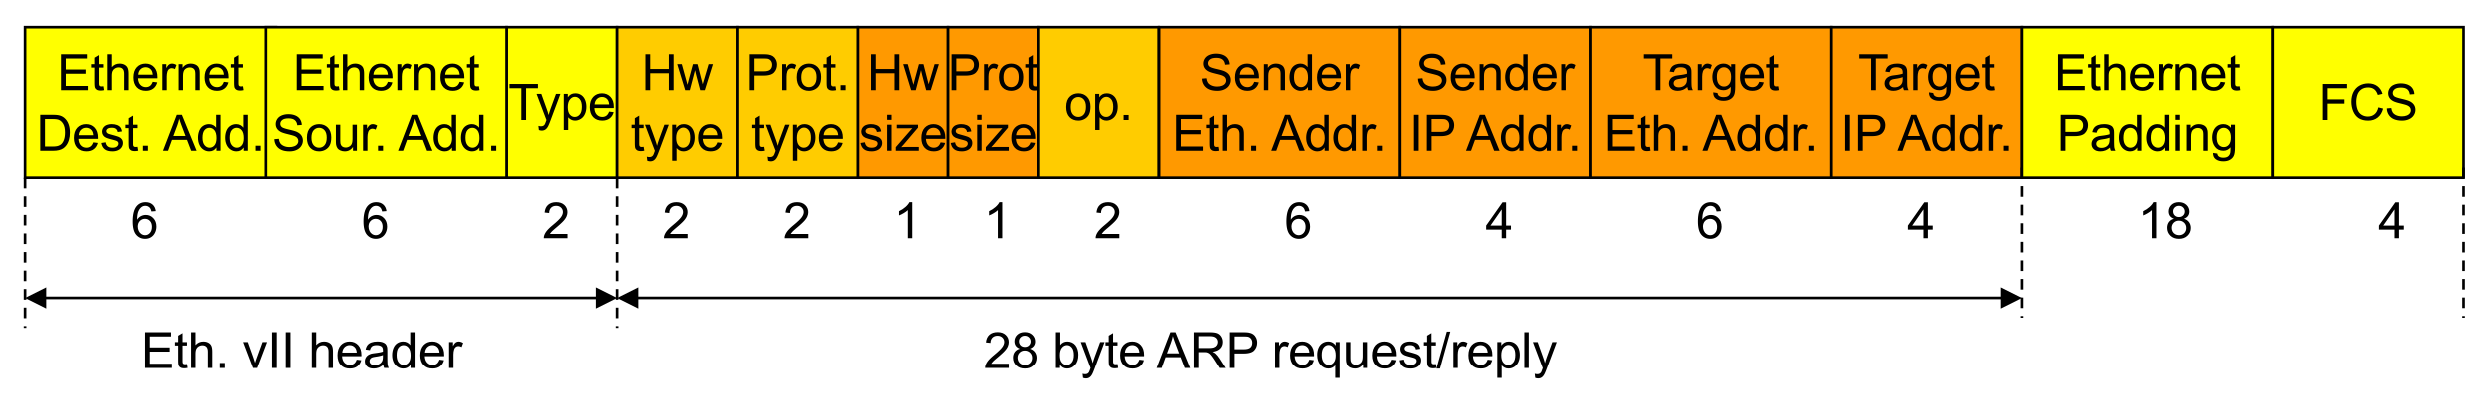
\includegraphics[width=1\textwidth]{images/frameethernet.png}
    \caption{Struttura di un frame Ethernet}
    \label{fig:frameethernet}
\end{figure}

Questo è il frame ethernet: 
in giallo ho l'header e la coda di ethernet , la coda svolge il ruolo di verificare che ci siano errori(fcs da 4 byte), il campo padding in coda serve a raggiungere i 64 byte(è un filler) minimi del frame totale tra ethernet e arp(arp è interno a l frame ethernet)
il frame deve avere una dimensione minima di 64 byte, il protocollo arp è quello arancione chiaro e scuro al centro.

Struttura del frame ethernet:
\begin{multicols}{2}
\begin{itemize}
    \item ethernet destination address: ind liv 2 del mittente - uguale a sender eth address
    \item ethernet source address
    \item type: tipologia tecnologia del livello 2
    \item hw type: specifica l'hardware che si sta usando al livello 2
    \item protocol type: specifica che procollo si vuole convertire dal liv 3 al 2(quindi non ha utilizzo esclusivo per indirizzi ip)
    \item hw size: dimensione indirizzo di liv 3
    \item prot size: dimensione indirizzo liv 2
    \item options:
    \item sender ethernet address: indirizzo liv 2 del mittente
    \item sender ip address: indirizzo liv 3 del mittente
    \item target ethernet address: indirizzo liv 2 del destinatario
    \item target ip address: indirizzo liv 3 del destinatario
    \item op: operazione che si vuole effettuare, 1 per richiesta arp, 2 per risposta arp
\end{itemize}
\end{multicols}

\subsubsection{Esempio ARP all'interno di una rete}

\begin{figure}[h!]
    \centering
    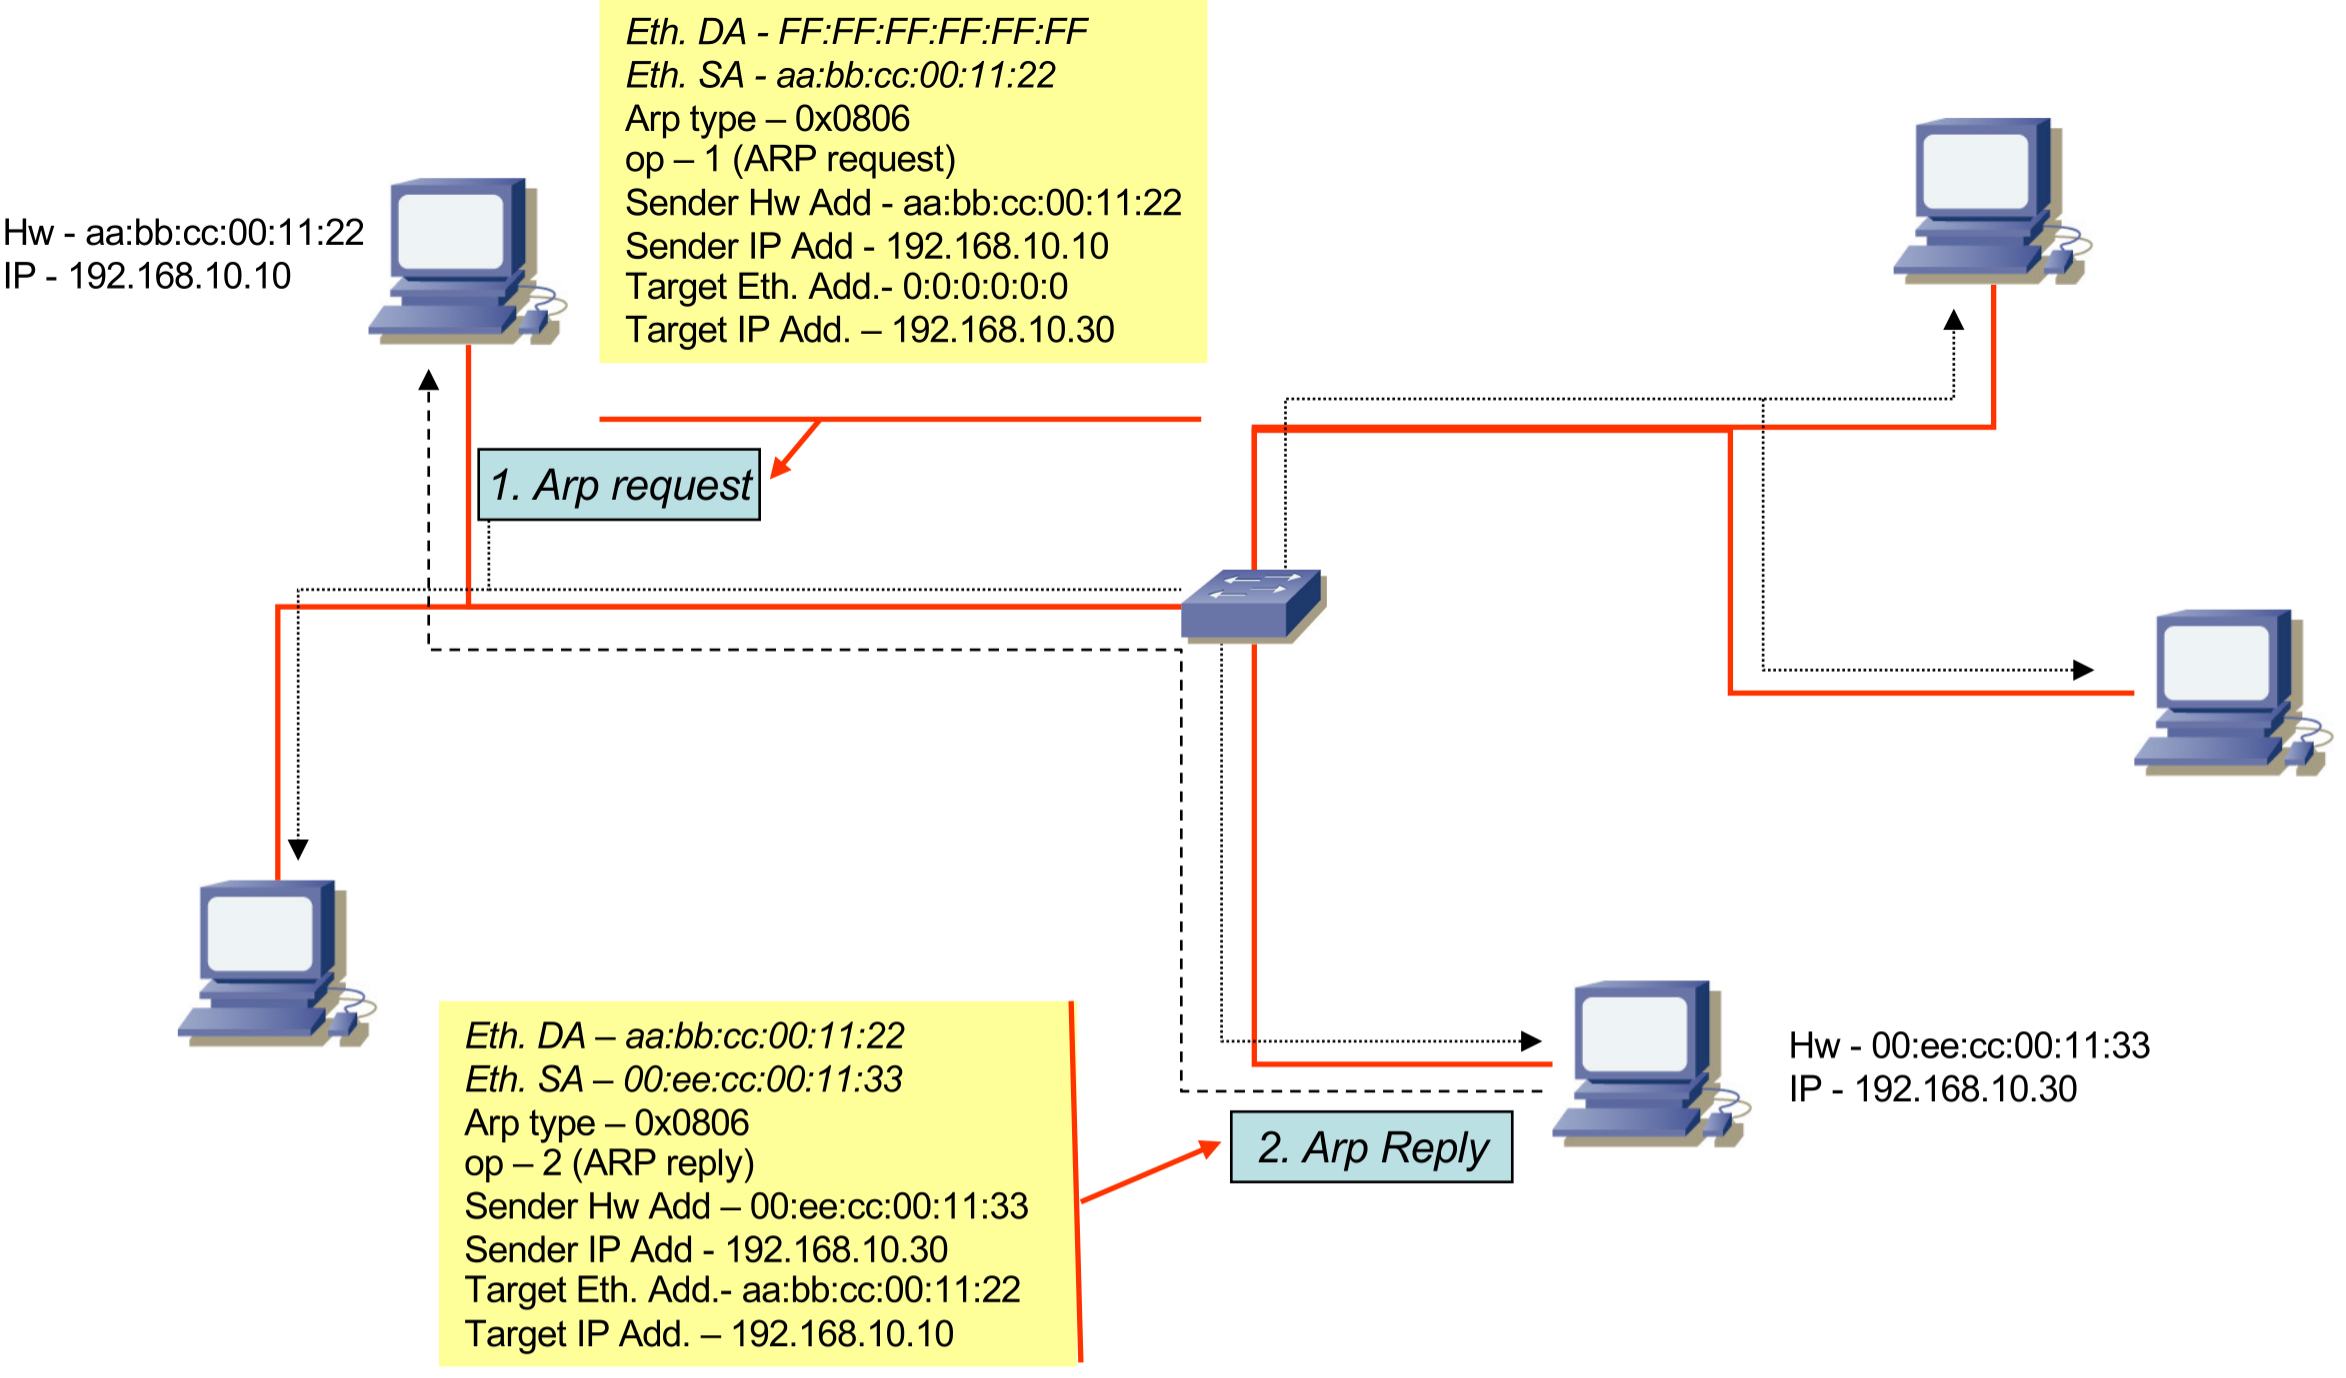
\includegraphics[width=1\textwidth]{images/esempioarp.png}
    \caption{Esempio di funzionamento del protocollo ARP}
    \label{fig:esempioARP}
\end{figure}

L'indirizzo hw è l'indirizzo fisico anche detto mac, è tipicamente in esadecimali ed è di 6 byte.

I riquadri in giallo sono pacchetti ARP utili alla comunicazione tra i due pc(visto che il dispositivo sta utilizzando arp per inviare un pacchetto allora sta usando un arp request, che viene segnato come op - 1 nel frame ethernet); i pacchetti in giallo quindi incapsulano una serie di informazioni del frame ethernet. 

Inoltre l'Ethernet destination address viene impostato a ff:ff:ff:ff:ff:ff (broadcast per indirizzi ARP) se viene effettuata un'ARP Request, questo perchè il mittente sta cercando di individuare l'indirizzo fisico del destinatario, di cui conosce solo l'ip, perciò utilzza ARP.

Nel momento della ARP request non so l'indirizzo ethernet del destinatario, ma so solo l'indirizzo ip, quindi ho tutti i byte del Ethernet address del target a 0.

Manderò quindi in broadcast(quindi multicast: a tutti i dispositivi della rete)(linee non tratteggiate) una richiesta a tutti i computer della rete, aspettando che il computer con l'indirizzo ip corrispondete a quello del target mi invii in unicast(linea tratteggiata) con un altro pacchetto ARP(arp reply, op - 2).

A questo punto il computer che ha inviato inizialmente l'ARP request riceve le info necessarie per poter inviare il pacchetto al destinatario. 
\newpage
\subsubsection{Esempio ARP in reti diverse}
IMPORTANTE: IL TCP(livello 4) si disinteressa di questo percorso, opera come se A e B fossero già collegati(end to end).

\begin{figure}[h!]
    \centering
    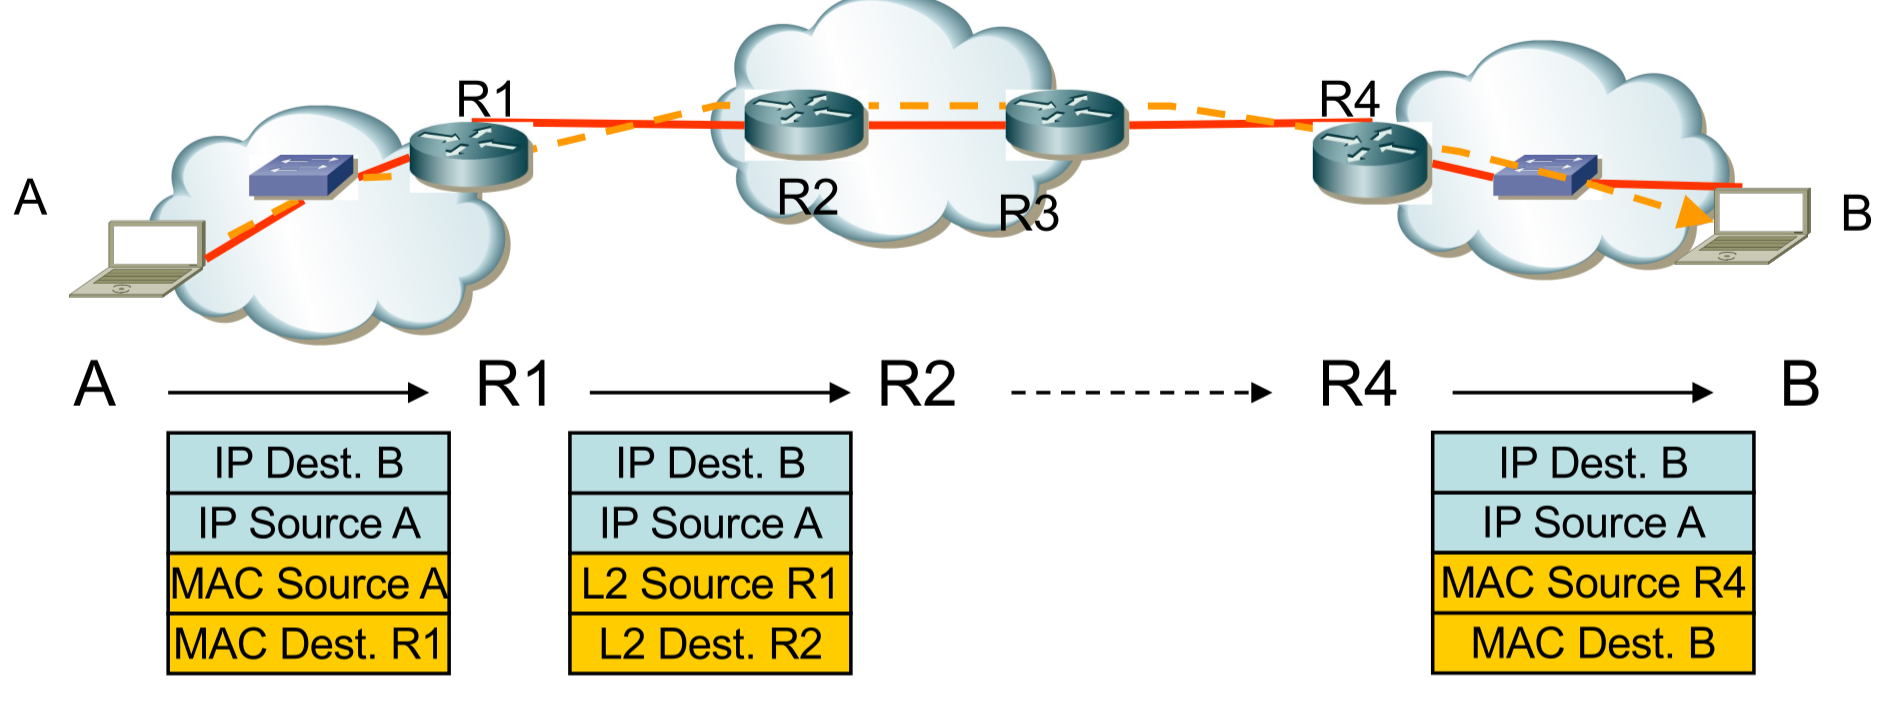
\includegraphics[width=1\textwidth]{images/esempioARPretidiverse.png}
    \caption{Esempio di funzionamento del protocollo ARP tra reti diverse}
    \label{fig:esempioARPretidiverse}
\end{figure}

\paragraph{Default gateway e tabelle di routing}

per scoprire se la rete del destinatario è la stessa da cui mando la richiesta arp: applico la mia maschera di rete all’ip del destinatario(la mia maschera di rete è un informazione che posseggo). quindi se la rete del destinatario non corrisponde a quella del mittente, per “uscire” e connettermi all’altra rete devo passare per il router. gli indirizzi di livello 3, quindi l’ip del destinatario e l’ip del mittente sono info che non variano tra un passaggio da un router all’altro, mentre quelli in giallo, gli indirizzi fisici(mac) variano tra router all’altro.
quindi il protocollo arp verrà applicato ad ogni passaggio tra un router all'altro cambiando quindi i mac source e mac destinatario, inserendo i mac dei dispositivi(router) tra cui avviene questo passaggio d’informazione. fino ad arrivare al dispositivo con l’indirizzo ip contenuto nel frame (ip dest B)
Il primo router a cui ci appoggiamo per l'inoltramento del pacchetto viene chiamato default gateway.

I router servono a connettere reti diverse, quindi se il destinatario non è nella mia rete allora mi appoggio al router, che ha un indirizzo ip di default, che è il default gateway.

Le tabelle di routing sono delle tabelle che i router utilizzano per sapere come inoltrare i pacchetti verso le reti di destinazione. Queste tabelle contengono informazioni sulle reti raggiungibili, i loro indirizzi IP e fisici.

A fine processo B legge i livelli 2 e 3 e riconosce i propri indirizzi MAC e IP, a quel punto può leggere il payload del pacchetto, che contiene i dati che A voleva inviare a B.

\paragraph{ARP nella stessa rete}
Se nel processo in cui cerco di capire se il destinatario sta nella mia rete o no scopro che sta nella mia rete allora non mi serve il router e posso inviare direttamente il pacchetto al destinatario, ma prima devo scoprire il suo indirizzo fisico(mac), quindi applico arp come fatto inizialmente.

\newpage
\subsection{Dynamic Host Configuration Protocol (DHCP) - configurazione automatica degli indirizzi IP tramite server DHCP}

 Un indirizzo ip può essere statico o dinamico, servers e router hanno tipicamente indirizzi statici.

Gli ind statici si configurano manualmente, quelli dinamici invece sono configurati tramite DHCP, un server che va configurato dall'utente ed è utile perchè fornisce: 
\begin{multicols}{3}
\begin{itemize}
    \item indirizzo ip del dispositivo
    \item netmask
    \item indirizzo ip del router
    \item indirizzo ip del server DNS
    \item lease time
\end{itemize}
\end{multicols}
Il lease time è il tempo in cui l'indirizzo ip è riservato al dispositivo, dopo di che il dispositivo deve richiedere un nuovo indirizzo ip;
è anche possibile ottenere un indirizzo IP riservato, sulla base dell'indirizzo fisico MAC.

\paragraph{DHCP relay - inoltro delle richieste DHCP}
Se nella rete locale non è disponibile un DHCP server, allora la richiesta può essere inoltrata  verso un'altra rete che dispone della funzione DHCP relay.

\paragraph{DHCP - funzionamento}
Questo protocollo fa uso dei UDP per la comunicazione tra client e server, e funziona in modo simile a ARP.

L'host che desidera un undirizzo IP si affida a questo protocollo per ottenerlo, inviando un messaggio DHCP discover, incapsulandolo in un pacchetto UDP, che viene inviato in broadcast a tutti i dispositivi della rete locale.

All'interno del pacchetto UDP, il mittente inserisce i seguenti indirizzi IP:
\begin{itemize}
    \item IP source address: l'indirizzo IP del mittente, che non è ancora stato assegnato, viene impostato momentaneamente a 0.0.0.0
    \item IP destination address: l'indirizzo IP del server DHCP, viene impostato a 255.255.255.255
\end{itemize}

Tutti gli eventuali server DHCP presenti nella rete rispondono in broadcast con un messaggio DHCP offer, che contiene le informazioni richieste dal client, come l'indirizzo IP assegnato, la netmask ecc\dots

Il client riceve le offerte dai server DHCP e sceglie una di esse, inviando un messaggio DHCP request al server scelto.

Infine il server DHCP conferma l'assegnazione dell'indirizzo IP con un messaggio DHCP ack.

    \begin{figure}[h!]
    \centering
    \includegraphics[width=1\textwidth]{images/dhcp.png}
    \caption{Funzionamento del protocollo DHCP}
    \label{fig:dhcp}
\end{figure}

\subsection{Zero-configuration networking}

Il zero-configuration networking è la configurazione della rete in assenza di server e amministratori, è ideale solo per reti piccole e semplici. Non è quindi un protocollo alternativo a DHCP.

\paragraph{Link-Local Address}
La IANA ha riservato a questo scopo un Link-Local Address: 169:254.0.0/16 

Gli indirizzi IP dei dispositivi nella rete vengono assegnati automaticamente, all'interno di un range specifico: [169.254.1.1 - 169.254.254]

\paragraph{ARP probe}
Quando un dispositivo si connette alla rete, invia un ARP probe per verificare se l'indirizzo IP scelto è già in uso. Se non riceve risposta, assume che l'indirizzo sia disponibile e lo utilizza. 
Se un altro host ha lo stesso indirizzo, sceglie casualmente un altro indirizzo IP all'interno dello stesso range.

\paragraph{ARP announcement}
Dopo aver scelto un indirizzo IP, il dispositivo invia un ARP announcement per informare gli altri dispositivi della rete del suo nuovo indirizzo. 

Questi indirizzi sono di tipo riservato e non possono essere usati per comunicare fuori dalla rete locale.



\subsection{Network Address Translation (NAT) - da IP privato a IP pubblico}


Il NAT è un software eseguito dal router di frontiera(ha il compito di far uscire dalla rete locale i pacchetti destinati ad indirizzi ip di altre reti).

Quindi è quel servizio che converte l'indirizzo privato del router di frontiera, in uno pubblico, cosè da comunicare con “l'esterno”. 
Perciò i router di frontiera delle altre reti non vedono l'indirizzo privato ma quello pubblico, convertito grazie al NAT.

Più precisamente, il NAT è una famiglia di tecniche/protocolli.

\paragraph{Funzionamento del NAT e tabelle di traduzione}

Tutti i datagram IP che viaggiano da (verso) la LAN hanno il medesimo indirizzo IP
mittente (destinazione), poichè il router di frontiera ha un solo indirizzo IP pubblico, che viene utilizzato per tutte le comunicazioni in uscita (entrata) dalla rete locale(LAN).

Il NAT utilizza una tabella di traduzione per mappare gli indirizzi IP privati della rete locale con l'indirizzo IP pubblico del router di frontiera; utilizzando le porte come ulteriore identificativi.

\begin{figure}[h!]
    \centering
    \includegraphics[width=0.85\textwidth]{images/nat.png}
    \caption{Funzionamento del NAT: traduzione degli indirizzi IP privati in indirizzi IP pubblici}
    \label{fig:nat}
\end{figure}

\newpage

\subsection{Internet control message protocol (ICMP) - diagnostica della rete}
I messaggi ICMP si dividono messaggi di errore e messaggi di richiesta; vengono inviati attraverso i pacchetti IP(protocol type 1);
questo protocollo serve a segnalare informazioni di controllo relative al livello di rete, un messaggio ICMP è composto dai campi type e code:
\begin{multicols}{2}
\begin{itemize}
    \item type: indica il tipo di messaggio ICMP
    \item code: dettagli sul tipo di messaggio
\end{itemize}
\end{multicols}


\begin{figure}[h!]
    \centering
    \includegraphics[width=0.67\textwidth]{images/comandiicmp.png}
    \caption{Principali comandi ICMP e loro utilizzo}
    \label{fig:comandiicmp}
\end{figure}



\paragraph{Esempio utilizzo di ICMP - ping}
Ad esempio, echo request e echo reply sono alla base del comando ping.
Type 8 corrisponde a echo request, mentre type 0 corrisponde a echo reply. 

\begin{figure}[h!]
    \centering
    \includegraphics[width=0.55\textwidth]{images/pingicmp.png}
    \caption{Esempio di funzionamento di ICMP tramite il comando ping}
    \label{fig:pingicmp}
\end{figure}
\paragraph{Esempio utilizzo di ICMP - traceroute}
Tramite il traceroute( utilizzo dei ICMP type 11) scopro il percorso che sta seguendo il pacchetto 
comandi: traceroute sitoweb

\begin{figure}[h!]
    \centering
    \includegraphics[width=0.8\textwidth]{images/traceroute.png}
    \caption{Esempio di funzionamento di ICMP tramite il comando traceroute}
    \label{fig:traceroute}
\end{figure}
\newpage




\section{Algoritmi di routing}




%\chapter{Livello 2 Data link}

\section{Strategie di controllo errore}
\subsection{Distinzione tra strategie di controllo errori}
I pacchetti di livello 2 sono chiamati frame/trame, sono divisi in header e trailer; nel trailer sono presenti i campi utili alle strategie di controllo degli errori.

È possibile distinguere due tipi principali di strategie:
\begin{enumerate}
    \item FEC (Forward Error Correction): il mittente invia dati ridondanti, in modo che il destinatario possa correggere gli errori senza richiedere una ritrasmissione.
    \item ARQ (Automatic Repeat-reQuest): il mittente invia i dati e il destinatario richiede la ritrasmissione dei dati corrotti. 
\end{enumerate}
\subsection{ARQ (Automatic Repeat-reQuest)}
Nei sistemi di telecomunicazioni, Automatic Repeat-reQuest è una strategia di controllo di errore, che svolge il compito di rivelare un errore (ma non di correggerlo). I pacchetti corrotti vengono scartati e viene richiesta la loro ritrasmissione.

I protocolli di tipo ARQ più comuni sono:
\begin{itemize}
    \item Stop-and-Wait 
    \item Go-Back-N 
    \item Selective Repeat
\end{itemize}


\newpage
\subsubsection{Stop-and-Wait}
Lo stop-and wait è un protocollo di tipologia Continous ARQ, per cui è ammessa la trasmissione continua di più frame numerati.

In questo caso specifico, i segnali di riscontro negativi sono cumulativi.

\begin{figure}[htbp]
    \centering
    \begin{minipage}{0.4\textwidth}
        \includegraphics[width=\linewidth]{images/stopwait.png}
        \caption{Schema Stop-and-Wait}
    \end{minipage}%
    \hfill
    \begin{minipage}{0.55\textwidth}
        Il protocollo Stop-and-Wait prevede che il mittente attenda il riscontro del destinatario per ogni frame inviato, prima di procedere con il frame successivo.

        Il mittente invia una trama, quindi si ferma (stop) e attende (wait) il riscontro (Ack) da parte del ricevente prima di trasmettere una nuova trama.
\begin{itemize}
    \item $T_f$: tempo di trasmissione di una trama [s]
    \item $T_{ACK}$: tempo di trasmissione di un riscontro [s]
    \item $T_p$: tempo di elaborazione di una trama [s]
    \item $\tau$: tempo di propagazione [s]
\end{itemize}
    \end{minipage}
\end{figure}

\paragraph{Efficienza di stop and wait in assenza di errori}

Prima di definire l'efficienza del protocollo, è necessario definire il tempo necessario a trasmettere una trama:

\begin{equation}
T_{tot} = T_f + T_{ACK} + 2T_p + 2\tau
\end{equation}

$T_p$ come già detto è il tempo di elaborazione della trama, dipende dalla valocità di elaborazione e quindi non dovrebbe essere precisamente uguale in trasmissione e ricezione, ma per semplicità lo consideriamo uguale.
Inoltre $T_f$, il tempo di trasmissione della trama, è anche definito come il tempo utile, poichè tutti gli altri tempi che consideriamo sono relativi a operazioni di controllo,elaborazione e invio del pacchetto
L'efficienza ($\eta$) è perciò definita come:
\begin{equation}
\eta = \frac{T_f}{T_{tot}} = \frac{T_f}{T_f + T_{ACK} + 2T_p + 2\tau}
\end{equation}

Si possono effettuare alcune semplificazioni, considerando che $T_{ACK}$ e $T_p$ sono molto più piccoli di $T_f$ e $\tau$, quindi possiamo considerare:

\begin{equation}
T_{tot} = T_f + 2\tau
\end{equation}
da cui si ottiene l'efficienza:

\begin{equation}
\eta = \frac{T_f}{T_f + 2\tau} = \frac{1}{1 + \frac{2\tau}{T_f}} = \frac{1}{1 + \alpha} 
\end{equation}
dove $\alpha$ = $\frac{2\tau}{T_f}$ è il rapporto di propagazione normalizzato

\begin{itemize}
    \item il throughput è pari al prodotto tra la frequenza di cifra C (capacità del canale) e l'efficienza: $\eta$C
    \item anche in assenza di errori, l'efficienza non è mai pari a 1.
\end{itemize}

\newpage

\paragraph{Efficienza di stop and wait in presenza di errori}

I problemi che possono verificarsi sono:
\begin{multicols}{2}
\begin{itemize}
    \item il frame o l'ACK arrivano errati
    \item il frame non arriva
\end{itemize}
\end{multicols}

\begin{figure}[htbp]
    \centering
    \begin{minipage}{0.48\textwidth}
        \includegraphics[width=\linewidth]{images/erroreframe.png}
        \caption{Errore nel frame: quando si verifica un errore nel frame, il mittente si accorge del problema grazie alla scadenza del timer avviato durante la trasmissione. 
        In tal caso, il frame viene ritrasmesso. Questo processo garantisce che i dati vengano ricevuti correttamente, ma può ridurre l'efficienza del protocollo a causa delle ritrasmissioni necessarie.}
    \end{minipage}%
    \hfill
    \begin{minipage}{0.48\textwidth}
        \includegraphics[width=\linewidth]{images/erroreack.png}
        \caption{Errore nell'ACK: quando si verifica un errore nell'ACK, il mittente non riceve il riscontro atteso entro il tempo stabilito dal timer. 
        Anche in questo caso, il frame viene ritrasmesso. }
    \end{minipage}
\end{figure}

Come calcolo il $T_{out}$(time che avvio nel momente nella trasmissione del frame)?

Deve valere almeno il tempo di invio del ACK($T_{ACK}$), più il tempo di propagazione(andata e ritorno) più il tempo di elaborazione del frame($T_p$, in ricezione e trasmissione):
\begin{equation}
T_{out} \geq T_{ACK} + 2\tau + 2T_p
\end{equation}

Il numero di frame ritrasmessi per la corretta ricezione del frame è detto $N_S$ ed è in media considerabile come una variabile aleatoria;

inoltre il numero totale di frame trasmessi($N_R$) è dato dal numero di frame ritrasmessi più il frame inviato con successo:
\begin{equation}
N_R = N_S + 1
\end{equation}


Definiamo il frame error rate(FER), come la probabilità che un frame venga ricevuto con errore, FINIRE E APPROFONDIRE

\newpage
\subsubsection{Protocolli Continuous ARQ}
I protocolli continuous ARQ, a differenza dello stop-and-wait, prevede l'invio di un'insieme di pacchetti(frame/trame) numerati, tramite sliding window.
Vengono definite:
\begin{itemize}
    \item finestra di trasmissione $W_s$: definisce la grandezza della finestra di ricezione, perciò quanti pacchetti posso inviare "consecutivamente"(on the fly, in attesa di riscontro) e da cui posso aspettarmi un riscontro (ACK) cumulativo
    \item finestra di ricezione  $W_R$: definisce la grandezza della finestra di ricezione, 
\end{itemize} 
Se il campo dedicato alla numerazione è costituito da b bit, si potranno
numerare in modo differente fino a $N_b$ trame. 


\subsubsection{Go-Back-N}
\paragraph{Senza errori - efficienza massima}
Il protocollo Go-Back-N è un protocollo di tipo Continuous ARQ, che consente la trasmissione continua di più frame numerati. In questo caso specifico, i segnali di riscontro negativi sono cumulativi.

Nel caso in cui ci siano errori allora questo protocollo prevede di ritornare indietro nel momento della trasmissione in cui c'è stato l'errore(alla trama N), perciò go back N.
\begin{figure}[htbp]
    \centering
    \begin{minipage}{0.4\textwidth}
        \includegraphics[width=\linewidth]{images/gobackinsenzaerrori.png}
        \caption{Go-Back-N senza errori}
    \end{minipage}%
    \hfill
    \begin{minipage}{0.55\textwidth}
        Nel seguente esempio la finestra di tramissione è 3 e quella di ricezione 1; vengono riscontrati gli ack in modo corretto nei tempi previsti dalla finestra, che nel frattempo ad ogni ack corretto ricevuto scorre di posizione.
        
        Questo vuol dire che nel caso in cui non ci siano errori con l'invio delle trame e con il riscontro degli ack, il seguente protocollo ha efficienza massima.
 
    \end{minipage}
\end{figure}
 \newpage
\subsubsection{Con errori}
Si possono riscontrare errori durante la ricezione del pacchetto e durante il riscontro degli ack; a seconda della tipologia dell'errore avremo soluzioni differenti.
\paragraph{Errore trasmissione del frame} utilizzo del negative ACK (NACK)
\begin{figure}[htbp]
    \centering
    \begin{minipage}{0.4\textwidth}
        \includegraphics[width=\linewidth]{images/gobackinerrori.png}
        \caption{Go-Back-N con errori in trasmissione}
    \end{minipage}%
    \hfill
    \begin{minipage}{0.55\textwidth}
        Quando si verifica un errore in un frame, il destinatario scarta il frame errato e tutti i frame successivi. 
        
        Il mittente, una volta rilevato l'errore(tramite la ricezione di un NACK(negative ACK) inviato dal destinatario), ritrasmette il frame errato e tutti i frame successivi.
    \end{minipage}
\end{figure}

\paragraph{Errore trasmissione - ACK non ricevuto ($T_{out}$)} caso in cui l'ACK non venga inviato o si sia perso

\begin{figure}[htbp]
    \centering
    \begin{minipage}{0.55\textwidth}
        L'unico modo con il quale il mittente può evitare che il sistema si blocchi in caso di mancato riscontro(neanche NACK),  è quello di avviare un timer ad ogni frame inviato, entro il quale va ricevuto un riscontro.
        
        Se questo timer($T_{out}$) scade allora la finestra torna indietro e ritrasmette da dove è stato riscontrato il problema.
    \end{minipage}%
    \hfill
    \begin{minipage}{0.4\textwidth}
        \includegraphics[width=\linewidth]{images/gobacknerroreack.png}
        \caption{Go-Back-N con errore nell'ACK}
    \end{minipage}
\end{figure}

\newpage

\paragraph{Errore trasmissione - ACK equivocato($T_{out}$, )}
\begin{figure}[htbp]
    \centering
    \begin{minipage}{0.55\textwidth}
        Quando si verifica un equivoco nell'ACK, il mittente interpreta erroneamente il riscontro ricevuto e potrebbe ritrasmettere frame già ricevuti correttamente dal destinatario. 
        Questo equivoco può portare a un aumento delle ritrasmissioni e a una riduzione dell'efficienza del protocollo.
    \end{minipage}%
    \hfill
    \begin{minipage}{0.4\textwidth}
        \includegraphics[width=\linewidth]{images/equivocoack.png}
        \caption{Go-Back-N con equivoco nell'ACK}
    \end{minipage}
\end{figure}


\newpage
\section{Livello 2 Frame DHLC}


\subsection{Struttura del frame}
\begin{figure}[h!]
    \centering
    \includegraphics[width=0.8\textwidth]{images/strutturaframe.png}
    \caption{Struttura del frame HDLC}
    \label{fig:struttura-frame}
\end{figure}
\begin{itemize}
    \item flag: sono posti ad inizio e fine frame così da delimitare il frame e far capire a chi lo riceve quando inizia e quando finisce il frame, questi flag sono SEMPRE 8 bit in questa sequenza: 
01111110, ossia 7E in esadecimale
        \item address: indirizzo del trasmettitore, ricevitore o broadcast(se tutti 1)

    \begin{multicols}{2}
        \item control: indica il tipo di frame
        \item information: dati del livello superiore, payload
        \item FCS(frame check sequence): 
    \end{multicols}
\end{itemize}

\vspace{1em}
\noindent\rule{\linewidth}{0.4pt}
\vspace{1em}

\subsection{Bit stuffing}
 A proposito dei flag usati nel frame(011111110) che succede se questa sequenza invece fa parte della informazione utile del frame e non come flag delimitatore?

\begin{figure}[h!]
    \centering
    \includegraphics[width=0.8\textwidth]{images/bitstuffing.png}
    \caption{Esempio di bit stuffing}
    \label{fig:bit-stuffing}
\end{figure}
Risolvo inserendo uno 0 ogni cinque 1 ripetuti; questo fa perdere la molteplicità di 8 del frame.

\newpage

\subsection{Controllo degli errori casuali con CRC}

HDLC numera i frame e usa il protocollo di linea, utilizzando 3 o 7 bit, usando una tecnica di piggybacking per gestire il flusso che viene dalla direzione opposta(finestre di trasmissione e ricezione).

Il CRC è un metodo per il calcolo di somme di controllo (checksum). Il nome deriva dal fatto che i dati d'uscita sono ottenuti elaborando i dati di ingresso i quali vengono fatti scorrere ciclicamente in una rete logica.

Sfrutta l'algebra dei campi finiti ed è utile per l'individuazione di errori casuali nella trasmissione dati (a causa di interferenze, rumore di linea, distorsione), il CRC non è invece affidabile per verificare la completa correttezza dei dati contro tentativi intenzionali di manomissione.
\paragraph{Polinomio generatore}
Un codice CRC è definito dal suo polinomio generatore di ordine r:

esempio r = 3

\begin{equation}
    G(x) = x^3 + x^2 + 1 \quad \Rightarrow \quad 1101
\end{equation}

\subsubsection{Cosa avviene in trasmissione}
 Con una scelta opportuna del polinomio generatore è possibile rilevare errori sul singolo bit etc... ;

 setup del CRC per la trasmissione:

\begin{figure}[htbp]
    \centering
    \begin{minipage}{0.45\textwidth}
        Traduco i bit che compongono header e payload in un polinomio P(x) di coefficienti d; perciò di grado d-1.
    \end{minipage}%
    \hfill
    \begin{minipage}{0.5\textwidth}
        \includegraphics[width=\linewidth]{images/crctrasmissione.png}
        \caption{Schema del calcolo di CRC, P(x)}
    \end{minipage}
\end{figure}

\begin{figure}[htbp]
    \centering
   \begin{minipage}{0.5\textwidth}
        \includegraphics[width=\linewidth]{images/crcricezione.png}
        \caption{Schema del calcolo di CRC, $x^rP(x)$}
    \end{minipage}
    \hfill
     \begin{minipage}{0.45\textwidth}
        Si moltiplica P(x), ricavato qui sopra, per $x^r$(shift di r posizioni, le stesse del poliniomio generatore), ottendo il polinomio $x^rP(x)$ di grado d+r-1, con coefficienti d+r.
      
        In seguito allo shift, il campo FCS del frame sarà costutuito da r zeri.
    \end{minipage}%
\end{figure}

\paragraph{Calcolo e verifica del CRC in trasmissione}
In trasmissione si divide il polinomio $x^rP(x)$ per G(x), il resto di questa operazione[il polinomio R(x)] sono i bit del CRC, da inserire nel FCS del frame.
Vedi operatore XOR appendice basi.

\begin{equation}
    \frac{x^rP(x)}{G(x)} = Q(x) \oplus \frac{R(x)}{G(x)}
\end{equation}


\begin{figure}[htbp]
    \centering
    \begin{minipage}{0.45\textwidth}
        \includegraphics[width=\linewidth]{images/calcolocrc.png}
        \caption{Inserimento bit in FCS}
        \label{fig:calcolo-crc}
    \end{minipage}%
    \hfill
    \begin{minipage}{0.5\textwidth}
        Devo quindi inserire i bit del polonomio R(x) all'interno del FCS, effettuo l'operazione:
\begin{equation}
    P^{Tx} = x^rP(x) \oplus R(x)
\end{equation}
    \end{minipage}
\end{figure}
\newpage


 \subsubsection{Esempio calcolo CRC}
    \begin{figure}[htbp]
        \centering
        \includegraphics[width=0.8\textwidth]{images/esempiocrc.png}
        \caption{Esempio di calcolo CRC}
        \label{fig:esempio-crc}
    \end{figure}

\vspace{0.3em}
\noindent\rule{\linewidth}{0.4pt}
\vspace{0.3em}

\subsubsection{Verifica CRC}

C'è la necessità di verificare se il CRC calcolato ed inserito nel FCS sia corretto.
\paragraph{Polinomio relativo} è necessario calcolare il polonomio relativo $P^{Rx}(x)$ per verificare CRC; questo polinomio non è altro che la trama di (d+r-1) bit ricevuti in ricezione.
\paragraph{Condizione necessaria}
Infine per verificare CRC c'è da tenere a mente la condizione necessaria affinchè il CSC sia corretto, ossia che il resto della divisione tra polinomio relativo[$P^{Rx}(x)$] e polonomio generatore[G(x)] sia nullo:

\begin{equation}
    \frac{P^{Rx}(x)}{G(x)} = Q'(x) \oplus R'(x)
\end{equation}
Può accadere che il resto sia nullo con trama ricevuta errata (la condizione è necessaria, non sufficiente). 

Non si può quindi essere certi della correttezza della trama (c'è sempre una
probabilità non nulla di falso positivo).

Se il resto NON è nullo, invece, c'è la certezza che la trama sia errata
perché la condizione necessaria è stata violata

\paragraph{Dimostrazione condizione necessaria}
Nel caso in cui la trama ricevuta sia corretta, il polinomio che costruiamo da questa trama deve essere uguale al polinomio originale(trama trasmessa), cioè:
\begin{equation}
    P^{Rx}(x) = P^{Tx}(x)
\end{equation}

Se effettuiamo la divisione per il polinomio generatore:

    \begin{equation}
        \frac{P^{Rx}(x)}{G(x)} = \frac{P^{Tx}(x)}{G(x)} = \frac{x^rP(x) \oplus R(x)}{G(x)} = \frac{x^rP(x)}{G(x)} \oplus \frac{R(x)}{G(x)}
    \end{equation}
    \begin{equation}
        \frac{P^{Rx}(x)}{G(x)} = \frac{x^rP(x)}{G(x)} \oplus \frac{R(x)}{G(x)} = Q(x) \oplus \frac{R(x)}{G(x)} \oplus \frac{R(x)}{G(x)} = Q(x)
    \end{equation}

   

    \subsection{Protocollo point to point (PPP)}

    \begin{figure}[htbp]
        \centering
        \includegraphics[width=0.85\textwidth]{images/pointtopoint.png}
        \caption{Protocollo Point to Point}
        \label{fig:point-to-point}
    \end{figure}

Il protocollo Point to Point è comunemente usato nello stabilire connessioni dirette tra due nodi.

Il frame è quasi identico a quello del HDLC, ha un campo aggiuntivo, quello protocol: specifica il protocollo di livello 3 che stiamo trasportando.

\paragraph{Network bit order - Big Endian e Little Endian}
A differenza dello standard HDLC, big-endian, il protocollo PPP non è endianness specifico.

L'ordine dei byte (conosciuto anche come big-endian, little-endian o middle-endian a seconda dei metodi differenti), in informatica, indica modalità differenti usate dai calcolatori per immagazzinare all'interno della memoria dati di dimensione superiore al byte;dipende essenzialmente dall'architettura hardware usata.

"I termini big-endian e little-endian derivano dai nomi di due popolazioni che abitavano nelle favolose isole di Lilliput e Blefuscu nel romanzo I viaggi di Gulliver di Jonathan Swift. Queste erano entrate in rivalità per il modo in cui aprivano le uova - rompendo la punta o il fondo: a Lilliput, per editto dell'imperatore il cui figlio una volta si tagliò aprendo un uovo dall'estremità più grande, fu ordinato di aprire le uova dall'estremità più piccola (little endians); a Blefuscu si rifugiarono gli oppositori che volevano conservare la tradizione di rompere le uova dall'estremità più grande (big endians). A causa di questa differenza e della sua legittimazione imperiale era scoppiata tra le due isole una guerra sanguinosa."

\begin{figure}[htbp]
    \centering
    \includegraphics[width=0.8\textwidth]{images/endian.png}
    \caption{Big Endian e Little Endian}
    \label{fig:endian}
\end{figure}
\newpage

    \subsubsection{Byte stuffing}


    Anche qui, vista la struttura del pacchetto molto simile a quella del frame HDLC, c'è il rischio di confondere il dato informativo con un flag; perciò si attua il byte stuffing.

    \paragraph{Sequenza di flag 0x7d}

    Se si vuole evitare la sequenza 0x7e (01111110), si antepone la sequenza di controllo 0x7d (01111101); al posto della sequenza 0x7e inseriamo la sua versione in XOR con la sequenza 0x20 (00100000).
    
    A quel punto avremo individuato la sequenza "pericolosa" all'interno del frame, ossia 0x7e, avremo un identificativo, 0x7d, che ci dice dov'è situata nel frame e la sostituiremo con il suo valore in XOR con 0x20.
     
    Quindi quando all'interno del frame leggo il byte 0x7d, il nuovo flag che indica che c'è stato byte stuffing, non leggiamo 0x7d ma il byte successivo, quello calcolato tramite il 0x7e XOR 0x20.

    In ricezione se applico nuovamente XOR 0x20 al byte precedentemente modificato con lo XOR, allora otterrò nuovamente il byte iniziale, 0x7e.
    
    
    
    \begin{figure}[htbp]
        \centering
        \includegraphics[width=1\textwidth]{images/bytestuffing.png}
        \caption{Esempio di byte stuffing}
        \label{fig:byte-stuffing}
    \end{figure}

    Nel caso in cui incappiamo con una "falsa" sequenza di flag del byte stuffing, ossia 0x7d, la trasmettermo come 0x7d, 0x5d.
     
    \subsubsection{Struttura PPP}

    Il PPP utilizza due protocolli per la gestione del collegamento tra nodi:
    
    \begin{figure}[htbp]
        \centering
        \begin{minipage}{0.45\textwidth}
            \includegraphics[width=\linewidth]{images/pppencapsulation.png}
            \caption{Encapsulation PPP}
            \label{fig:ppp-encapsulation}
        \end{minipage}%
        \hfill
        \begin{minipage}{0.5\textwidth}
            \begin{itemize}
                \item LCP(Link Control Protocol): grazie al quale si apre la connessione, si ha la verifica della qualità del collegamento e rende possibile l'autenticazione(PAP o CHAP)
                \item NCP(Network Control Protocol): con cui è possible scegliere e configurare uno o più protocolli di rete(es. IP)
            \end{itemize} 

        \end{minipage}
    \end{figure}
\newpage
    \subsubsection{Autenticazioni}
    \begin{figure}[htbp]
        \centering
        \includegraphics[width=1\textwidth]{images/autenticazionecapchap.png}
        \caption{Autenticazione PAP e CHAP}
        \label{fig:autenticazione-pap-chap}
    \end{figure}
    \paragraph{Autenticazione PAP} 
    Password Authentication Protocol (PAP) invia username e password in chiaro. È semplice ma poco sicuro, poiché le credenziali possono essere intercettate(password e username sono solitamente criptate).

    \paragraph{Autenticazione CHAP} 
    Challenge Handshake Authentication Protocol (CHAP) utilizza un meccanismo di challenge-response con hash per autenticare in modo più sicuro, evitando di trasmettere la password in chiaro.


\section{Protocolli di accesso}
A livello due viene svolto un ruolo importante dai protocolli di accesso, che possono essere di due tipologie:
\begin{itemize}
    \item Accesso ordinato:
    \begin{itemize}
        \item Ogni nodo ha un turno prestabilito per trasmettere, evitando collisioni.
        \item Utilizzato in sistemi come il polling o il token passing.
        \item Garantisce un utilizzo equo del canale, ma può introdurre ritardi se un nodo non ha dati da trasmettere.
    \end{itemize}
    \item Accesso casuale:
    \begin{itemize}
        \item senza rilevazione del canale:
        \begin{itemize}
            \item I nodi trasmettono senza verificare se il canale è libero.
            \item Può portare a collisioni frequenti, come nel protocollo ALOHA puro.
        \end{itemize}
        \item con rilevazione del canale:
        \begin{itemize}
            \item senza rivelazione di collisioni:
            \begin{itemize}
                \item I nodi verificano se il canale è libero prima di trasmettere.
                \item Non rilevano collisioni, quindi i dati persi devono essere ritrasmessi dopo un timeout.
                \item Esempio: Carrier Sense Multiple Access (CSMA).
            \end{itemize}
            \item con rilevazione di collisioni:
            \begin{itemize}
                \item I nodi verificano se il canale è libero e rilevano eventuali collisioni durante la trasm.
                \item In caso di collisione, interrompono la trasm. e ritentano dopo un intervallo casuale.
                \item Esempio: CSMA/CD (utilizzato in Ethernet).
            \end{itemize}
        \end{itemize}
    \end{itemize}
\end{itemize}
\newpage

\subsection{Troughput di rete}
Per valutare le prestazioni di una rete vengono considerati parametri come \dots;
il Troughput, tra questi, è uno dei più rilevanti: è definito come il numero di bit al secondo che giungono corretti; maggiore è questo valore, meglio è per le prestazioni della rete.

Questo valore è alto quando gli errori nei pacchetti che giungono a destinazione sono pochi.

Nota bene: a livello 4 si preferisce in genere utilizzare il
goodput definito come bit al secondo che giungono corretti,
ma riferiti alla sola informazione utile del livello applicativo. Il
throughput invece tiene conto anche di tutti gli header aggiunti
ai vari livelli della pila protocollare.


\subsubsection{Calcolo del Troughput}

Per il calcolo del Troughput è fondamentale definire alcuni concetti:
\begin{itemize}
    \item frequenza di cifra C: è un paramentro tipico del livello 2 (datalink), rappresenta la capacità del canale su cui sta viaggiando l'informazione, quindi la quantità di bit che possono fisicamente muoversi all'interno del canale
    \item Troughput massimo: è pari alla frequenza di cifra C
    \item $\Lambda_s$: è il numero medio di pacchetti emessi dalla sorgente
    \item $\pi$: la probabilità che il pacchetto arrivi errato o che non arrivi proprio
    \item $\Lambda_T$: Troughput medio
\end{itemize}
\paragraph{Troughput medio packet/s}
Il Troughput medio $\Lambda_T$,misurato in pacchetti al secondo, si calcola come:

\begin{equation}
    \Lambda_T = \Lambda_s (1 - \Pi) \quad \text{[packet/s]}
\end{equation}
\paragraph{Troughput medio bit/s}
se desiderassi calcolare il Troughput medio misurato in bit al secondo, ho bisogno di definire il parametro L, ossia la lunghezza media dei pacchetti, allora il Troughput vale:

\begin{equation}
    \Gamma_T = \Lambda_s L (1 - \Pi) \quad \text{[bit/s]}
\end{equation}
\paragraph{Troughput adimensionale}
è anche possibile definire un valore adimensionale del Troughput, che vari da un valore utile che va da 0 ad uno massimo di 1; lo si ottiene normalizzando $\Gamma_s$ alla capacità del canale C; inoltre definiamo:
\begin{itemize}
    \item $T = \frac{L}{C}$ è il tempo medio di trasmissione di un singolo pacchetto
    \item $G = \Gamma_sT$ è il traffico medio normalizzato emesso dalla sorgente
\end{itemize}


\begin{equation}
    S = \frac{\Lambda_s L}{C}(1 - \Pi) = \frac{\Lambda_T}{C} = G(1 - \Pi)
\end{equation}

se S è maggiore di 1 significa che il mittente sta ricevendo più bit di quelli che il canale può supportare.

\newpage

\subsection{Protocollo ALOHA puro}
ALOHA è un protocollo di accesso multiplo casuale senza rilevazione del canale.

Questo protocollo non prevede vincoli all'invio di dati e quindi all'occupazione della banda. Quando una postazione ha dati da trasmettere, li trasmette.

Poiché ogni stazione agisce indipendentemente dalle altre, il successo è determinato unicamente dalla mancata collisione con altre trasmissioni da parte di altre stazioni. Poiché i canali broadcast danno la possibilità di verificare (feedback) se il frame trasmesso è stato ricevuto correttamente oppure se si sono verificate collisioni, la stazione trasmittente ascolta il canale e determina il successo o l'insuccesso della trasmissione. Le stazioni si mettono in attesa di un riscontro (ack) da parte del ricevente. Se ci sono collisioni (o se l'ack non arriva entro un tempo di attesa stabilito), i frame corrotti vengono distrutti. Ciò indipendentemente dal livello di corruzione dei dati; quando un frame è stato interessato da collisione, viene eliminato. In questo caso la postazione mittente reinvia il frame dopo un'attesa casuale e si rimette in ascolto sul canale (o attende un ack) fino a quando non stabilisce che il frame è stato ricevuto correttamente.
\subsubsection{Collisioni nel canale condiviso}
\begin{figure}[htbp]
    \centering
    \includegraphics[width=0.8\textwidth]{images/alohacollisioni.png}
    \caption{Collisioni nel protocollo ALOHA}
    \label{fig:aloha-collisioni}
\end{figure}

Le stazioni trasmittenti inviano i loro messaggi lungo il canale condiviso. Se l'intervallo di tempo durante il quale due o più stazioni trasmettono si sovrappone, allora si avrà una collisione; quindi le stazioni coinvolte non riceveranno alcun ack e dovranno perciò ritentare la trasmissione in un istante successivo. 

Per evitare che la collisione si ripeta indefinitamente è opportuno che le stazioni coinvolte tentino la loro ritrasmissione in tempi distinti, in modo da ridurre la probabilità di nuove sovrapposizioni fra i due periodi di trasmissione.

\newpage
\subsubsection{Calcolo del Troughput di ALOHA puro}
Si ipotizza che le stazioni trasmettono sul canale secondo un processo di Poisson, quindi ognuna di esse è un evento indipendente dagli altri; le stazioni trasmettono pacchetti nel canale indipendentemente da ciò che fanno le altre stazioni.

Si suppone anche che ci sia un numero di stazioni molto elevato, che trasmettano tutte nel canale condiviso di interesse; 

ricordando la formula del Troughput medio espresso in pacchetti al secondo: 

\begin{equation}
    \Lambda_T = \Lambda_s (1 - \pi) \quad \text{[packet/s]}
\end{equation}

ci interessa capire quanto può valere $(1 - \pi)$ nel protocollo ALOHA puro, quindi la probabilità che i pacchetti arrivino a destinazione considerando solamente l'effetto della collisione tra pacchetti, non altri fenomeni, poichè si vuole valutare solo l'effetto del protocollo ALOHA sul Troughput.

Per fare ciò considero un nuovo parametro, il periodo di vulnerabilità.

\begin{figure}[htbp]
    \centering
    \begin{minipage}{0.45\textwidth}
        \includegraphics[width=\linewidth]{images/periodovulnerabilita.png}
        \caption{Periodo di vulnerabilità}
        \label{fig:periodo-vulnerabilita}
    \end{minipage}%
    \hfill
    \begin{minipage}{0.5\textwidth}
        Il periodo di vulnerabilità rappresenta l'intervallo di tempo durante il quale una trasmissione(pacchetti verde chiaro) può essere soggetta a collisioni(pacchetto P collide con la trasmissione se rientra nella finestra di 2T). Nel caso del protocollo ALOHA puro, questo periodo è pari a $2T$, dove $T$ è il tempo di trasmissione di un singolo pacchetto. Durante questo intervallo, se un'altra stazione inizia a trasmettere, si verifica una collisione.
    \end{minipage}
\end{figure}

Il valore $(1 - \pi)$ rappresenta quindi la probabilità per la quale nell'intervallo di trasmissione di un pacchetto questo arrivi correttamente(infatti 1 - $\pi$, dove 1 è la probabilità massima per la quale non ci sia collisione, $\pi$ invece rappresenta la probabilità di collisione, più è alta e più andrà a diminuire il valore ideale 1).


Dall'espressione di Poisson($p_0$ rappresenta la probabilità che zero eventi (collisione di pacchetti) si verifichino in un certo intervallo di tempo) si calcola che la probabilità di non avere eventi di collisione nell'intervallo di vulnerabilità 2T è la seguente: 

\begin{equation}
p_k = \frac{(\Lambda t)^k}{k!} e^{-\Lambda t} \Rightarrow p_0 = \frac{(\Lambda_s 2T)^0}{0!} e^{-\Lambda_s 2T} = e^{-2\Lambda_s T} = (1 - \pi)
\end{equation}
\paragraph{Troughput in packet/s}
sostituendolo nella formula di $\Lambda_T$:

\begin{equation}
\Lambda_T = \Lambda_s (1 - \Pi) = \Lambda_s p_0 = \Lambda_s e^{-2 \Lambda_s T} \quad \text{packet/s}
\end{equation}

\paragraph{Troughput in bit/s}

\begin{equation}
    \Gamma_T = \Lambda_s L (1 - \pi) = \Lambda_s L (e^{-2\Lambda_s T}) \quad \text{[bit/s]}
\end{equation}

\paragraph{Troughput adimensionale}

\begin{equation}
    S = \frac{\Lambda_s L}{C}(1 - \Pi) = \frac{\Lambda_T}{C} = G(1 - \Pi) = G(e^{-2\Lambda_s T})
\end{equation}
\newpage

\subsubsection{Prestazioni ALOHA puro}

\paragraph{Andamento funzione $G(e^{-2\Lambda_s T})$} analizzando la funzione 

\begin{figure}[htbp]
    \centering
    \begin{minipage}{0.5\textwidth}
        \includegraphics[width=\linewidth]{images/funzionealoha.png}
        \caption{Andamento Troughput normalizzato ALOHA puro}
        \label{fig:funzione-aloha}
    \end{minipage}%
    \hfill
    \begin{minipage}{0.45\textwidth}
        La funzione $S = G e^{-2G}$ ha un massimo per $G = 0.5$, che corrisponde a $S = 0.184$.
        
        Questo significa che il massimo Troughput normalizzato ottenibile con ALOHA puro è circa il 18.4\% della capacità del canale, un valore molto basso dovuto all'elevata probabilità di collisione.
        
        Le prestazioni basse sono dovute al fatto che le stazioni trasmettono senza alcun controllo sul canale.
    \end{minipage}
\end{figure}
\subsubsection{Appendice matematica - distribuzione di Poisson}
La distribuzione di Poisson $\mathcal{P}_\lambda(n)$ è una distribuzione di probabilità discreta data da
\begin{equation}
\mathcal{P}_\lambda(n) = \frac{\lambda^n e^{-\lambda}}{n!} \quad \text{per ogni } n \in {N},
\end{equation}
dove $\lambda$ è il numero medio di eventi per intervallo di tempo, mentre $n$ è il numero di eventi per intervallo di tempo (lo stesso col quale si misura $\lambda$) di cui si vuole la probabilità.

\paragraph{Esempio} Un call center riceve in media 4 chiamate all'ora. Qual è la probabilità che riceva esattamente 2 chiamate in un'ora? ($\lambda = 4$ , $n = 2$)

\begin{equation*}
\mathcal{P}_4(2) = \frac{4^2 \cdot e^{-4}}{2!} = \frac{16 \cdot e^{-4}}{2} \approx \frac{16 \cdot 0.0183}{2} \approx \frac{0.2928}{2} \approx 0.1464
\end{equation*}

\begin{figure}[h!]
    \centering
    \includegraphics[width=0.8\textwidth]{images/poissongrafico.png}
    \caption{Grafico della distribuzione di Poisson}
    \label{fig:poisson_grafico}
\end{figure}

\newpage

\subsection{Protocollo ALOHA slotted - prestazioni}

Il protocollo Slotted Aloha aggiunge al protocollo Aloha (da cui deriva) un'ulteriore caratteristica, ovvero la suddivisione del tempo in intervalli discreti chiamati slot. 

Ogni stazione è vincolata a cominciare la propria trasmissione all'inizio di uno slot temporale.

Se una stazione ad un certo istante è pronta a trasmettere dovrà attendere necessariamente l'inizio del successivo slot. La conseguenza di tale caratteristica è che due trasmissioni o collidono completamente all'interno dello stesso slot oppure non collidono affatto; il problema delle collisioni parziali non c'è.


\begin{figure}[htbp]
    \centering
    \includegraphics[width=0.77\textwidth]{images/slottedaloha.png}
    \caption{Protocollo ALOHA slotted}
    \label{fig:slotted-aloha}
\end{figure}



\begin{figure}[htbp]
    \centering
    \begin{minipage}{0.43\textwidth}
        \includegraphics[width=\linewidth]{images/periodoslotted.png}
        \caption{Protocollo ALOHA slotted}
        \label{fig:slotted-aloha}
    \end{minipage}%
    \hfill
    \begin{minipage}{0.45\textwidth}
        \paragraph{Probabilità di collisione}
        Il modello è identico a quello visto per ALOHA, ma stavolta il tempo di vulnerabilità
        si è dimezzato per cui la probabilità di non avere tentativi di trasmissione in T
        \begin{equation}
            p_0 = \frac{(\Lambda_s T)^0}{0!} e^{-\Lambda_s T} = e^{-\Lambda_s T}
        \end{equation}
    \end{minipage}
\end{figure}

\begin{figure}[htbp]
    \centering
    \begin{minipage}{0.425\textwidth}
        \includegraphics[width=\linewidth]{images/slottedgrafico.png}
        \caption{Protocollo ALOHA slotted}
        \label{fig:slotted-aloha}
    \end{minipage}%
    \hfill
    \begin{minipage}{0.45\textwidth}
        \paragraph{Troughput normalizzato}

\begin{equation}
    S = \Lambda_s \frac{L}{C}p_0 = \Lambda_s \frac{L}{C}e^{-\Lambda_s T} = G e^{-\Lambda_s T}
\end{equation}

Il protocollo Slotted Aloha ha come conseguenza il dimezzamento del periodo di vulnerabilità, che in tal caso è pari a T. L'efficienza massima risulta conseguentemente raddoppiata, pari quindi al 36,8\%.

    \end{minipage}
\end{figure}

\newpage


\subsection{Protocolli Carrier Sense Multiple Access - CSMA (rilevazione canale)}

I protocolli CSMA sono quei protocolli di accesso che rilevano il canale prima di trasmettere, per migliorare l'efficienza ed evitare collisioni con altre trasmissioni.
 
Se rilevando il canale, risulta occupato, allora la stazione può attuare diverse strategie: 
\begin{itemize}
    \item 1-persistent:  continuare a "sentire" il canale finché non lo rileva libero per trasmettere subito dopo
    \item no-persistent: rinviare la trasmissione ad un momento successivo, generalmente scegliendo un intervallo di attesa casuale
    \item p-persistent: scegliere di comportarsi con probabilità p in una delle due modalità precedenti
\end{itemize}
"Può accadere di rilevare il canale come libero, ma nel tempo in cui l'ho rilevato e ho iniziato ad utilizzarlo qualcun'altro potrebbe iniziare a sua volta la comunicazione, c'è quindi da considerare il tempo che impiega l'onda elettromagnetica a viaggiare nel mezzo $v$ e noi a rilevarla $T_p$".

\subsubsection{CSMA/CD - CSMA with collision detection}
Per realizzare il CSMA/CD è necessario che la stazione possa a livello fisico
realizzare una comunicazione full duplex (per essere in grado a livello fisico di
trasmettere e ricevere contemporaneamente, per permettere il listening while talking spiegato successivamente).

La stazione che intende trasmettere verifica che il canale sia libero prima di
trasmettere (sensing del canale del CSMA); 
\paragraph{Listening while talking}
se il canale è libero si trasmette la trama e durante la trasmissione della stessa
(tra l'invio del primo e dell'ultimo bit) si continua ad ascoltare il canale (Listening
while talking)(ascolta se stessa).



\begin{figure}[htbp]
    \centering
    \begin{minipage}{0.5\textwidth}
        \includegraphics[width=\linewidth]{images/esempiocsmacd.png}
        \caption{Esempio CSMA/CD}
        \label{fig:csma-cd}
    \end{minipage}%
    \hfill
    \begin{minipage}{0.45\textwidth}
        \paragraph{Rilevazione collisione}
Se il segnale "ascoltato" (confronto tra le forme d'onda a livello fisico) è diverso
da quello trasmesso, si rileva la collisione (altra stazione che ha iniziato a
trasmettere sentendo il canale libero). 

In tal caso si può:

\begin{itemize}
    \item interrompere la trasmissione 
    \item inviare un segnale di jam per informare chi sta ascoltando il canale di scartare nel buffer di
ricezione tutti i bit della trama parziale ricevuta
\end{itemize}
    \end{minipage}
\end{figure}
\paragraph{Exponential backoff}
Il tempo di attesa per la rilevazione del canale in seguito ad una collisione viene calcolato in un intervallo $T_{slot}*[0;2^m-1]$ tramite un algoritmo di exponential backoff, per il quale $m = min(n;10)$, m è il numero di ritrasmissioni, n è il numero di collisioni consecutive , $T_{slot}$ è il tempo necessario a trasmettere un frame di lunghezza minima(512 bit). 




\newpage

\subsubsection{Dimostrazione funzionamento collision detection}
Utilizzando il CSMA/CD è necessario che i frame abbiamo una dimensione
superiore ad un valore minimo per garantire il funzionamento del collision
detection.
\begin{figure}[htbp]
    \centering
    \begin{minipage}{0.45\textwidth}
        \includegraphics[width=\linewidth]{images/dimostrazionecsma.png}
        \caption{Dimostrazione collision detection}
        \label{fig:dimostrazione-csma}
    \end{minipage}%
    \hfill
    \begin{minipage}{0.5\textwidth}



A e B comunicano nei tampi $\tau$(valore massimo, caso peggiore);
il primo bit inviato da A arriva a B dopo $\tau$ secondi.

Nel caso peggiore B ascolta il canale un istante($\epsilon$) prima che il bit di A arrivi a B, perciò B vedrà che il canale è libero, non sapendo che un'istante dopo arriveranno i bit di A, causando quindi una collisione.

B si accorge della collisione e manda un jam, impiegando $\tau$ per "avvisare" A.

A può apire che il jam che riceve è dovuto ad una collisione con la sua trasmissione solo se la sua trasmissione ($T_f$) dura almeno quanto il tempo che ha impiegato il suo primo bit di trasmissione ed il jam di B, perciò: $T_f  \geq 2\tau$ 

\begin{equation}
 T_f = \frac{L_f}{C} \geq 2\tau = \frac{2d}{v} \implies L_f \geq \frac{2dC}{v}
\end{equation}

        %Si supponga che A inizi a trasmettere al tempo t=0 e che B inizi a trasmettere al tempo $t = t_{prop}$ ($t_{prop}$ è il tempo di propagazione del segnale).

        %A rileverà la collisione al tempo $2t_{prop}$ (tempo necessario al segnale di B per raggiungere A).

        %Per garantire il funzionamento del collision detection, è necessario che A stia ancora trasmettendo quando rileva la collisione.

        %Quindi, la durata minima di un frame deve essere tale che la stazione trasmittente continui ad occupare il canale per almeno $2t_{prop}$.

        %Se la durata della trasmissione è inferiore a $2t_{prop}$, la collisione potrebbe non essere rilevata.
    \end{minipage}
\end{figure}
\subsubsection{CSMA/CA - CSMA with collision avoidance}
\paragraph{Duration}
L'obiettivo del CSMA/CA è diminuire il numero di collisioni.

In questa versione di CSMA, in cui c'è rilevazione del canale prima di trasmettere, se il canale è libero inizia la trasmissione inserendo la durata stimata della trasmissione del singolo frame (considerando anche i tempi di propagazione e la trasmissione del frame di riscontro) in un campo "duration" dell'header del frame.

\paragraph{Network allocation vector(NAV) - virtual sensing} Tutte le altre stazioni che condividono il canale ascoltano il frame e settano un
loro orologio interno, detto NAV, pari al valore del duration letto.

Finchè il NAV non si azzera non iniziano altre trasmissioni poiché si sa che il canale è occupato.
\begin{figure}[htbp]
    \centering
    \includegraphics[width=0.65\textwidth]{images/csmaca.png}
    \caption{CSMA/CA}
    \label{fig:csma-ca}
\end{figure}

%\newpage

%\section{Il Progetto IEEE 802}

Il progetto \textbf{IEEE 802} ha l’obiettivo di definire gli \textbf{standard per le reti locali (LAN)}, sia cablate che wireless, ed è stato successivamente esteso a:

\begin{itemize}
    \item \textbf{MAN} (Metropolitan Area Network), es. \texttt{IEEE 802.16} (WiMAX)
    \item \textbf{WPAN} (Wireless Personal Area Network), es. \texttt{IEEE 802.15} (Bluetooth)
\end{itemize}

\subsection*{Struttura della pila ISO/OSI nei livelli inferiori}
IEEE 802 si occupa dei \textbf{primi due livelli} del modello ISO/OSI:
\begin{enumerate}
    \item \textbf{Livello fisico (Physical Layer)}
    \item \textbf{Livello di collegamento dati (Data Link Layer)}
\end{enumerate}

Il livello Data Link viene ulteriormente suddiviso in:
\begin{itemize}
    \item \textbf{LLC (Logical Link Control)} -- definito dallo standard \texttt{IEEE 802.2}, è comune a tutte le tecnologie e fornisce un'interfaccia standard ai livelli superiori.
    \item \textbf{MAC (Media Access Control)} -- specifico per ciascuna tecnologia, definisce come accedere al mezzo trasmissivo.
\end{itemize}

\begin{figure}[h!]
    \centering
    \includegraphics[width=1\textwidth]{images/ieee802.png}
    \caption{Struttura della pila ISO/OSI secondo IEEE 802}
    \label{fig:ieee802}
\end{figure}

\subsection*{IEEE 802.1}
Lo standard \texttt{IEEE 802.1} definisce le \textbf{caratteristiche generali del progetto}, comprese le specifiche per la struttura degli \textbf{indirizzi MAC}.



\subsection*{Vantaggi della suddivisione LLC/MAC}
\begin{itemize}
    \item Favorisce la \textbf{modularità} e l'interoperabilità tra diversi tipi di rete.
    \item I protocolli di livello superiore (es. IP, TCP, UDP) possono utilizzare una singola interfaccia LLC, indipendentemente dallo standard MAC sottostante.
    \item Facilita l'\textbf{evoluzione tecnologica}, permettendo l'introduzione di nuovi standard MAC senza modificare gli strati superiori.
\end{itemize}


%\subsection{Livello LLC} Il livello LLC fornisce un'interfaccia unificata tra il livello Data Link e il livello Network (es. IP), indipendentemente dallo standard MAC sottostante (Ethernet, Wi-Fi, etc.).

%\subsubsection{Frame LLC}
%spiegazione

%\begin{figure}[h!]
%    \centering
%    \includegraphics[width=0.7\textwidth]{images/framellc.png}
%    \caption{Struttura del frame LLC}
%   \label{fig:framellc}
%\end{figure}


%\begin{figure}[h!]
%    \centering
%    \includegraphics[width=0.7\textwidth]{images/llcsnapframe.png}
%    \caption{Struttura del frame LLC SNAP}
%    \label{fig:llcsnapframe}
%\end{figure}


%\subsection{Livello MAC}

%\begin{figure}[h!]
%    \centering
%    \includegraphics[width=0.7\textwidth]{images/framemac.png}
%    \caption{Struttura del frame MAC}
%    \label{fig:framemac}
%\end{figure}

%\subsubsection{MAC address}

%\subsection{Ethernet}

%\begin{figure}[h!]
%    \centering
%    \includegraphics[width=0.7\textwidth]{images/ethernet.png}
%    \caption{Struttura del frame Ethernet}
%    \label{fig:ethernetframe}
%\end{figure}

%\subsubsection{Frame 802.3}

%\begin{figure}[h!]
%    \centering
%    \includegraphics[width=0.7\textwidth]{images/frame8023.png}
%    \caption{Struttura del frame 802.3}
%    \label{fig:frame8023}
%\end{figure}

%\subsubsection{Inter-frame gap}
%\begin{figure}[h!]
%    \centering
%    \begin{minipage}{0.5\textwidth}
%        \includegraphics[width=0.9\textwidth]{images/framegap.png}
%        \caption{Inter-frame gap}
%        \label{fig:framegap}
%    \end{minipage}\hfill
%    \begin{minipage}{0.45\textwidth}
%        Spazio tra i frame.
%    \end{minipage}
%\end{figure}


%\subsubsection{Ethernet a 10 Mbit/s}

%\subsubsection{Ethernet a 100 Mbit/s}

%\subsubsection{Ethernet a 1 Gbit/s}


%
\newpage

\section{Reti wireless}
Il wireless o senza fili indica una comunicazione tra dispositivi elettronici che non fa uso di cavi.

Generalmente il wireless utilizza onde radio a bassa potenza; tuttavia la definizione si estende anche ai dispositivi, meno diffusi, che sfruttano la radiazione infrarossa o il laser.

Ogni sistema di comunicazione wireless è composto da un trasmettitore, un ricevitore e dagli elementi deputati alla radiazione elettromagnetica ovvero alla trasduzione elettro-elettromagnetica e viceversa ovvero le antenne, i laser, i fotorivelatori.


\subsection{Wireless LAN - WLAN}
WLAN o wireless LAN è una rete locale (LAN) che sfrutta la tecnologia wireless, invece di una connessione cablata. In altre parole: con la sigla WLAN si indicano genericamente tutte le reti locali di computer che non utilizzano dei collegamenti via cavo per connettere fra loro gli host della rete; è una tecnologia definita da IEEE 802.11


\begin{multicols}{2}
    \begin{itemize}
        \item Pregi delle WLAN:
        \begin{itemize}
            \item Facilità di installazione
            \item Basso costo
            \item Assenza di cablaggio
            \item Mobilità
        \end{itemize}
    \end{itemize}
    \columnbreak
    \begin{itemize}
        \item Difetti delle WLAN:
        \begin{itemize}
            \item Inaffidabilità mezzo trasmissivo
            \item Sensibilità alle interferenze
            \item Privacy
        \end{itemize}
    \end{itemize}
\end{multicols}

\subsubsection{Infrastruttura WLAN}

"Il sistema è composto da un insieme di BSS interconnessi con un
Distribution System (DS) che collega i diversi Access Point (AP)"


\begin{figure}[h!]
    \centering
    \includegraphics[scale=0.2]{images/infrastrutturawlan.png}
    \caption{Infrastruttura WLAN}
    \label{fig:infrastrutturawlan}
\end{figure}
Nelle aree arancioni, dette Basic service set (BSS), le wireless station comunicano nello stesso canale radio; ciò che permette la comunicazione tra questa area con altre sono gli access point (AP). 

\paragraph{Access point} tramite il dispositivo access point è possibile che le tecnologie ethernet 802.3 e le tecnologie wireless 802.11 possano scambiarsi informazioni, fungendo da ponte tra rete cablata e rete wireless.

Funge tra ponte anche tra reti wireless con canali radio differenti, poiché il dato passa da un access point all'altro, utilizzando ethernet.

\newpage

\paragraph{Famiglia 802.11x}

\begin{figure}[htbp]
    \centering
    \begin{minipage}{0.45\textwidth}
        La famiglia 802.11x è uno standard IEEE che definisce le caratteristiche di una WLAN.

        Lo standard 802.11x definisce una serie di tecniche di modulazione radio per segnali half-duplex che utilizzano di base lo stesso formato di dati. In particolare, la trasmissione si basa sul controllo di collisioni CSMA/CA per cui una emittente su uno specifico canale è in grado di determinare se su quello stesso canale ci siano altre entità che stanno trasmettendo (anche su protocolli diversi da quelli definiti da 802.11x) e trasmette le sue trame dati solo se il canale in quel momento è libero.
    \end{minipage}
        \hfill
    \begin{minipage}{0.53\textwidth}
        \includegraphics[width=\linewidth]{images/famigliaieee802.png}
        \caption{802.11x}
    \end{minipage}
\end{figure}

\subsection{Struttura dei canali 802.11b}
Nello standard 802.11b la banda radio viene suddivisa in 14 canali, le "onde" rappresentano l'ampiezza di banda di ogni canale wireless.

Seguendo queste ampiezze si possono invididuare le terne di canali che non interferiscono tra di loro, ad esempio 1, 6, 11; a conti fatti ogni canale ha dopo 5 canali quello con cui non interferisce.

Queste terne coprono l'area di interesse della rete wireless senza avere interferenze.
\begin{figure}[h!]
    \centering
    \includegraphics[scale=0.225]{images/canali802.png}
    \caption{Struttura canali 802.11b}
    \label{fig:strutturacanali}
\end{figure}




\begin{figure}[h!]
    \centering
    \begin{minipage}{0.35\textwidth}
        \includegraphics[width=\linewidth]{images/cluster3celle.png}
    \end{minipage}
    \hfill
    \begin{minipage}{0.5\textwidth}
        \paragraph{Cluster}
        In questa rappresentazione ogni esagono rappresenta una cella o area di copertura di un access point (AP). I numeri all'interno degli esagoni indicano il canale utilizzato da ciascun AP.
        
        Questa configurazione permette di minimizzare le interferenze tra le celle adiacenti, ottimizzando le prestazioni della rete wireless.
    \end{minipage}
    \caption{Cluster di 3 celle (1,2,3)}
    \label{fig:cluster3celle}
\end{figure}
\newpage
\subsubsection{Distributed Coordination Function (DCF)}
La WLAN usa il CSMA/CA, la DCF è insieme di regole per la gestione dell’accesso al
mezzo condiviso.

\begin{figure}[h!]
    \centering
    \includegraphics[scale=0.25]{images/dcf.png}
    \caption{Distributed Coordination Function (DCF)}
    \label{fig:dcf}
\end{figure}

Source ha interesse di comunicare qualcosa(data) a destination, per farlo utilizza la tecnologia WNAL e perciò non può inviare direttamente l'informazione al destinatario ma lo fa attraverso un'ulteriore stazione, un access point(station with pending data to transmit).

Source ascolta il canale per un certo periodo prima di far partire la comunicazione(CSMA/CA), precisamente aspetta un tempo DIFS + backoff, rispettivamente:
\begin{itemize}
    \item DIFS(DCF inter frame space): specifica la modalità di CSMA/CA utilizzata dal sistema, specifica per 802.11  
    \item backoff time: tempo calcolato tramite algoritmo di backoff, per decidere il tempo di subentro in trasmissione, source e la stazione hanno dei backoff time diversi in questo caso
\end{itemize}
Nel momento in cui source inizia ad inviare i dati, il backoff time della stazione si interrompe(proseguirrà solo al termine della comuniazione tra source e destination, poichè comunicano grazie alla station).

Source aspetta un riscontro(ACK) da parte di destination, che attenderà per un tempo SIFS(Short inter frame space), ossia un tempo predefinito che viene fornito al destination per assicurarsi di aver terminato correttamente i processi di ricezione, pronto per trasmettere l'ACK nel modo più corretto possibile. Una volta ricevuto l'ACK, la comunicazione è terminata.

Quello che si vede successivamente nell'immagine, la "Contention with other stations", indica una possibile contesa con altre "source" per l'utilizzo della stazione per la tramissione.

C'è sempre contesa tra gli apparati per poter comunicare con questa tecnologia. 

\newpage
\subsection{Nodi nascosti ed esposti}
Questi problemi esistono poichè i nodi condividono gli stessi canali per la condivisione.
\paragraph{Nodo nascosto}
I nodi “nascosti” (A e C) comunicano con B; i frame collidono nei pressi del nodo B.
\begin{figure}[h!]
    \centering
    \begin{minipage}{0.49\textwidth}
        \includegraphics[width=\linewidth]{images/nodonascosto.png}
    \end{minipage}
    \hfill
    \begin{minipage}{0.5\textwidth}
        \paragraph{Nodo nascosto}
        Il nodo nascosto è un problema che si verifica nelle reti wireless quando due nodi non sono in grado di "vedersi" a vicenda a causa di ostacoli o distanza, ma entrambi possono comunicare con un terzo nodo. Ciò può portare a collisioni di pacchetti e perdita di dati.
    \end{minipage}
    \caption{Nodo nascosto}
    \label{fig:nodo nascosto}
\end{figure}

\subsubsection{Soluzione nodo nascosto} 

\begin{figure}[h!]
    \centering
    \begin{minipage}{0.5\textwidth}
\paragraph{Request to send RTS - 20 byte}
I nodi che intendono trasmettere tramite un nodo intermedio devono inviare un piccolo frame di richiesta, detto Request to send (RTS).

Inoltre la probabilità che ci sia una collisione, quindi un problema, con l'invio di questi pacchetti è molto bassa poichè sono molto piccoli.

\paragraph{Clear to send CTS - 14 byte}
Il nodo destinatario del frame RTS, conferma ed autorizza la richiesta inviando a sua volta un pacchetto piccolo, il Clear o send (CTS),  al nodo che ha inviato la richiesta.
    \end{minipage}
    \hfill
    \begin{minipage}{0.49\textwidth}
        \includegraphics[width=\linewidth]{images/soluzionenodonascosto.png}
    \end{minipage}
    \caption{Soluzione nodo nascosto}
    \label{fig:soluzionenodonascosto}
\end{figure}

\begin{figure}[h!]
    \centering
    \includegraphics[scale=0.2]{images/dcfhandshake.png}
    \caption{Handshake DCF per nodi nascosti}
    \label{fig:dcfhandshake}
\end{figure}
Esempio della tramissione WLAN  802.11 con RTS e CTS. Di fatto cambia solo il tempo della duration, prima era composta da data, SIFS e ACK; adesso includo i campi RTS e CTS come in figura.


\newpage

\paragraph{Nodo esposto}

\begin{figure}[h!]
    \centering
    \begin{minipage}{0.49\textwidth}
        \includegraphics[width=\linewidth]{images/nodoesposto.png}
    \end{minipage}
    \hfill
    \begin{minipage}{0.5\textwidth}
        \paragraph{Nodo esposto}
        A e B stanno comunicando ed occupano il canale; il nodo C vuole comunicare con il canale D ma sente, tramite rilevazione di canale, che questo è già occupato.

        Questo si risolve avviando un backoff time(casuale, secondo un algoritmo) a fine comunicazione trasmessa con successo così che tra un pacchetto e l'altro, di quelli inviati da A e B, ci sia "spazio" per le comunicazioni di C e D, che rilevavano il canale occupato.
    \end{minipage}
    \caption{Nodo esposto}
    \label{fig:nodo esposto}
\end{figure}


\subsection{Dispositivi wireless}

\subsubsection{Hub}
L'hub è un dispositivo che riceve i dati da una stazione e li ritrasmette a tutte le altre stazioni collegate. In ambito wireless, l'hub non viene praticamente mai utilizzato perché non è in grado di gestire le collisioni e non offre alcuna forma di filtraggio o instradamento dei dati. In generale, l'hub lavora a livello fisico (livello 1 ISO/OSI).

\subsubsection{Bridge}
Il bridge è un dispositivo che collega due segmenti di rete, anche di tipo diverso (ad esempio una rete cablata e una wireless), filtrando il traffico in base agli indirizzi MAC. In ambito wireless, il bridge permette di collegare due reti wireless o una rete wireless e una cablata, inoltrando solo i frame destinati all'altro segmento. Opera a livello data link (livello 2 ISO/OSI).

\subsubsection{Switch}
Lo switch è un dispositivo che riceve i frame e li inoltra solo alla porta (o interfaccia) corretta, in base all'indirizzo MAC di destinazione. In ambito wireless, la funzione di switch è spesso integrata negli access point avanzati, che possono gestire più connessioni e segmentare il traffico tra i dispositivi collegati. Anche lo switch opera a livello data link (livello 2 ISO/OSI).
\subsubsection{Modalità di funzionamento di uno switch}

\begin{itemize}
    \item \textbf{Store and Forward}:\\
    Lo switch legge l’intero frame e verifica il campo FCS (scarta il frame se errato). Il frame viene memorizzato temporaneamente nel buffer associato alla porta d’uscita e trasmesso quando la linea della porta d’uscita è libera.
    \item \textbf{Cut and Through}:\\
    Lo switch legge solo l’header del frame e inoltra immediatamente il frame senza memorizzazione intermedia. Il ritardo di elaborazione è indipendente dalla dimensione del frame.
    \item \textbf{Fragment Free}:\\
    Lo switch legge solo i primi 64 byte del frame (dimensione minima frame Ethernet) per evitare di inoltrare frame che potrebbero essere coinvolti in collisioni. I frame di dimensione minore a 64 byte vengono scartati.
\end{itemize}
CAPIRE SE FINIRE FILE 11
\end{document}